%% Adaptado a partir de :
%DIF LATEXDIFF DIFFERENCE FILE
%DIF DEL main-texto-proposta-antes.tex    Wed Nov  9 00:53:28 2022
%DIF ADD main-texto-proposta-depois.tex   Wed Nov  9 01:08:36 2022
%%    abtex2-modelo-trabalho-academico.tex, v-1.9.2 laurocesar
%% para ser um modelo para os trabalhos no IFSP-SPO

\documentclass[
    % -- opções da classe memoir --
    12pt,               % tamanho da fonte
    openright,          % capítulos começam em pág ímpar (insere página vazia caso preciso)
    %twoside,            % para impressão em verso e anverso. Oposto a oneside
    oneside,
    a4paper,            % tamanho do papel. 
    BIBLATEX,           % indica para utilizar BIBLATEX em vez do abntex2cite
    % -- opções da classe abntex2 --
    %chapter=TITLE,     % títulos de capítulos convertidos em letras maiúsculas
    %section=TITLE,     % títulos de seções convertidos em letras maiúsculas
    %subsection=TITLE,  % títulos de subseções convertidos em letras maiúsculas
    %subsubsection=TITLE,% títulos de subsubseções convertidos em letras maiúsculas
    % Opções que não devem ser utilizadas na versão final do documento
    %draft,              % para compilar mais rápido, remover na versão final
%   MODELO,             % indica que é um documento modelo então precisa dos geradores de texto
    TODO,               % indica que deve apresentar lista de pendencias 
    % -- opções do pacote babel --
    english,            % idioma adicional para hifenização
    brazil              % o último idioma é o principal do documento
    ]{ifsp-spo-inf-ctds}

        
% ---

% --- 
% CONFIGURAÇÕES DE PACOTES
% --- 
%\usepackage{etoolbox}
%\patchcmd{\thebibliography}{\chapter*}{\section*}{}{}
\usepackage{tabulary}
\usepackage{graphicx}
\graphicspath{ {./images/} }
\setlength {\marginparwidth }{2cm} 
%DIF 39c39
%DIF < 
%DIF -------
\usepackage{float} %DIF > 
%DIF -------
% carregando aqui referencias quando utilizando BIBLATEX
\IfPackageLoaded{biblatex}{%
\addbibresource{referencias.bib}
\addbibresource{exemplos/abntex2-doc-abnt-6023.bib}
}{}

% ---
% Informações de dados para CAPA e FOLHA DE ROSTO
% ---
%DIF 49c49
%DIF < \titulo{Sidekick - Gerenciador de clínica veterinária}
%DIF -------
\titulo{CertVet - Gerenciador de clínica veterinária} %DIF > 
%DIF -------

% Trabalho individual
%\autor{JOSÉ BRAZ DE ARAUJO}

% Trabalho em Equipe
% ver também https://github.com/abntex/abntex2/wiki/FAQ#como-adicionar-mais-de-um-autor-ao-meu-projeto
\renewcommand{\imprimirautor}{
    \begin{tabular}{lr}
        CAIQUE DANIEL FREITAS EUFRASIO DA SILVA & SP3046711 \\
        HENRIQUE HIROMI SHIMADA                 & SP3039421 \\
        IRINA CHANG GOUVEIA FERREIRA            & SP3058123 \\
        LUIS RENATO MOREIRA DA COSTA            & SP3035531 \\
        MARCOS QUERINO DOS SANTOS E SANTOS JUNIOR & SP3047245   \\
        MURILO SANTOS PIRES                     & SP3052737 \\
        WELEN MOTA SOUSA                        & SP146616X
    \end{tabular}
}


\tipotrabalho{Projeto da Disciplina Projeto Integrado I}

\disciplina{PI1A5 - Projeto Integrado I}

\preambulo{Desenho da aplicação para disciplina Projeto Integrado I}

\data{SETEMBRO DE 2022}

% Definir o que for necessário e comentar o que não for necessário
% Utilizar o Nome Completo, abntex tem orientador e coorientador
% então vão ser utilizados na definição de professor
\renewcommand{\orientadorname}{Professor:}
\orientador{ANTONIO AIRTON PALLADINO}
\renewcommand{\coorientadorname}{Professor:}
\coorientador{JOSÉ BRAZ DE ARAUJO}



% ---


% ---
% Configurações de aparência do PDF final


% informações do PDF
\makeatletter
\hypersetup{
        %pagebackref=true,
        pdftitle={\@title}, 
        pdfauthor={\@author},
        pdfsubject={\imprimirpreambulo},
        pdfcreator={LaTeX with abnTeX2},
        pdfkeywords={abnt}{latex}{abntex}{abntex2}{trabalho acadêmico}, 
        colorlinks=true,            % false: boxed links; true: colored links
        linkcolor=blue,             % color of internal links
        citecolor=blue,             % color of links to bibliography
        filecolor=magenta,              % color of file links
        urlcolor=blue,
        bookmarksdepth=4
}
\makeatother
% --- 

% ---

% ----
% Início do documento
% ----
%DIF PREAMBLE EXTENSION ADDED BY LATEXDIFF
%DIF UNDERLINE PREAMBLE %DIF PREAMBLE
\RequirePackage[normalem]{ulem} %DIF PREAMBLE
\RequirePackage{color}\definecolor{RED}{rgb}{1,0,0}\definecolor{BLUE}{rgb}{0,0,1} %DIF PREAMBLE
\providecommand{\DIFadd}[1]{{\protect\color{blue}\uwave{#1}}} %DIF PREAMBLE
\providecommand{\DIFdel}[1]{{\protect\color{red}\sout{#1}}}                      %DIF PREAMBLE
%DIF SAFE PREAMBLE %DIF PREAMBLE
\providecommand{\DIFaddbegin}{} %DIF PREAMBLE
\providecommand{\DIFaddend}{} %DIF PREAMBLE
\providecommand{\DIFdelbegin}{} %DIF PREAMBLE
\providecommand{\DIFdelend}{} %DIF PREAMBLE
\providecommand{\DIFmodbegin}{} %DIF PREAMBLE
\providecommand{\DIFmodend}{} %DIF PREAMBLE
%DIF FLOATSAFE PREAMBLE %DIF PREAMBLE
\providecommand{\DIFaddFL}[1]{\DIFadd{#1}} %DIF PREAMBLE
\providecommand{\DIFdelFL}[1]{\DIFdel{#1}} %DIF PREAMBLE
\providecommand{\DIFaddbeginFL}{} %DIF PREAMBLE
\providecommand{\DIFaddendFL}{} %DIF PREAMBLE
\providecommand{\DIFdelbeginFL}{} %DIF PREAMBLE
\providecommand{\DIFdelendFL}{} %DIF PREAMBLE
\newcommand{\DIFscaledelfig}{0.5}
%DIF HIGHLIGHTGRAPHICS PREAMBLE %DIF PREAMBLE
\RequirePackage{settobox} %DIF PREAMBLE
\RequirePackage{letltxmacro} %DIF PREAMBLE
\newsavebox{\DIFdelgraphicsbox} %DIF PREAMBLE
\newlength{\DIFdelgraphicswidth} %DIF PREAMBLE
\newlength{\DIFdelgraphicsheight} %DIF PREAMBLE
% store original definition of \includegraphics %DIF PREAMBLE
\LetLtxMacro{\DIFOincludegraphics}{\includegraphics} %DIF PREAMBLE
\newcommand{\DIFaddincludegraphics}[2][]{{\color{blue}\fbox{\DIFOincludegraphics[#1]{#2}}}} %DIF PREAMBLE
\newcommand{\DIFdelincludegraphics}[2][]{% %DIF PREAMBLE
\sbox{\DIFdelgraphicsbox}{\DIFOincludegraphics[#1]{#2}}% %DIF PREAMBLE
\settoboxwidth{\DIFdelgraphicswidth}{\DIFdelgraphicsbox} %DIF PREAMBLE
\settoboxtotalheight{\DIFdelgraphicsheight}{\DIFdelgraphicsbox} %DIF PREAMBLE
\scalebox{\DIFscaledelfig}{% %DIF PREAMBLE
\parbox[b]{\DIFdelgraphicswidth}{\usebox{\DIFdelgraphicsbox}\\[-\baselineskip] \rule{\DIFdelgraphicswidth}{0em}}\llap{\resizebox{\DIFdelgraphicswidth}{\DIFdelgraphicsheight}{% %DIF PREAMBLE
\setlength{\unitlength}{\DIFdelgraphicswidth}% %DIF PREAMBLE
\begin{picture}(1,1)% %DIF PREAMBLE
\thicklines\linethickness{2pt} %DIF PREAMBLE
{\color[rgb]{1,0,0}\put(0,0){\framebox(1,1){}}}% %DIF PREAMBLE
{\color[rgb]{1,0,0}\put(0,0){\line( 1,1){1}}}% %DIF PREAMBLE
{\color[rgb]{1,0,0}\put(0,1){\line(1,-1){1}}}% %DIF PREAMBLE
\end{picture}% %DIF PREAMBLE
}\hspace*{3pt}}} %DIF PREAMBLE
} %DIF PREAMBLE
\LetLtxMacro{\DIFOaddbegin}{\DIFaddbegin} %DIF PREAMBLE
\LetLtxMacro{\DIFOaddend}{\DIFaddend} %DIF PREAMBLE
\LetLtxMacro{\DIFOdelbegin}{\DIFdelbegin} %DIF PREAMBLE
\LetLtxMacro{\DIFOdelend}{\DIFdelend} %DIF PREAMBLE
\DeclareRobustCommand{\DIFaddbegin}{\DIFOaddbegin \let\includegraphics\DIFaddincludegraphics} %DIF PREAMBLE
\DeclareRobustCommand{\DIFaddend}{\DIFOaddend \let\includegraphics\DIFOincludegraphics} %DIF PREAMBLE
\DeclareRobustCommand{\DIFdelbegin}{\DIFOdelbegin \let\includegraphics\DIFdelincludegraphics} %DIF PREAMBLE
\DeclareRobustCommand{\DIFdelend}{\DIFOaddend \let\includegraphics\DIFOincludegraphics} %DIF PREAMBLE
\LetLtxMacro{\DIFOaddbeginFL}{\DIFaddbeginFL} %DIF PREAMBLE
\LetLtxMacro{\DIFOaddendFL}{\DIFaddendFL} %DIF PREAMBLE
\LetLtxMacro{\DIFOdelbeginFL}{\DIFdelbeginFL} %DIF PREAMBLE
\LetLtxMacro{\DIFOdelendFL}{\DIFdelendFL} %DIF PREAMBLE
\DeclareRobustCommand{\DIFaddbeginFL}{\DIFOaddbeginFL \let\includegraphics\DIFaddincludegraphics} %DIF PREAMBLE
\DeclareRobustCommand{\DIFaddendFL}{\DIFOaddendFL \let\includegraphics\DIFOincludegraphics} %DIF PREAMBLE
\DeclareRobustCommand{\DIFdelbeginFL}{\DIFOdelbeginFL \let\includegraphics\DIFdelincludegraphics} %DIF PREAMBLE
\DeclareRobustCommand{\DIFdelendFL}{\DIFOaddendFL \let\includegraphics\DIFOincludegraphics} %DIF PREAMBLE
%DIF COLORLISTINGS PREAMBLE %DIF PREAMBLE
\RequirePackage{listings} %DIF PREAMBLE
\RequirePackage{color} %DIF PREAMBLE
\lstdefinelanguage{DIFcode}{ %DIF PREAMBLE
%DIF DIFCODE_UNDERLINE %DIF PREAMBLE
  moredelim=[il][\color{red}\sout]{\%DIF\ <\ }, %DIF PREAMBLE
  moredelim=[il][\color{blue}\uwave]{\%DIF\ >\ } %DIF PREAMBLE
} %DIF PREAMBLE
\lstdefinestyle{DIFverbatimstyle}{ %DIF PREAMBLE
	language=DIFcode, %DIF PREAMBLE
	basicstyle=\ttfamily, %DIF PREAMBLE
	columns=fullflexible, %DIF PREAMBLE
	keepspaces=true %DIF PREAMBLE
} %DIF PREAMBLE
\lstnewenvironment{DIFverbatim}{\lstset{style=DIFverbatimstyle}}{} %DIF PREAMBLE
\lstnewenvironment{DIFverbatim*}{\lstset{style=DIFverbatimstyle,showspaces=true}}{} %DIF PREAMBLE
%DIF END PREAMBLE EXTENSION ADDED BY LATEXDIFF

\begin{document}

 
% Retira espaço extra obsoleto entre as frases.
\frenchspacing 

\pretextual

% ---
% Capa - Para proposta a folha de rosto é suficiente pois é mais completa.
% ---
\imprimirfolhaderosto
% ---

%DIF >  ---
%DIF >  inserir lista de ilustrações
%DIF >  ---
\DIFaddbegin \pdfbookmark[0]{\listfigurename}{lof}
\listoffigures*
\cleardoublepage
%DIF >  ---

%DIF >  ---
%DIF >  inserir lista de tabelas
%DIF >  ---
\pdfbookmark[0]{\listtablename}{lot}
\listoftables*
\cleardoublepage
%DIF >  ---

%DIF > ---
%DIF >  inserir lista de quadros
%DIF > ---
\pdfbookmark[0]{\listofquadros}{lot}
\listofquadros*
\cleardoublepage
%DIF > ---


\DIFaddend % ----------------------------------------------------------
% ELEMENTOS TEXTUAIS
% ----------------------------------------------------------
\tableofcontents*
\textual
\chapter[Introdução]{Introdução}

    \DIFdelbegin \DIFdel{Os }\DIFdelend \DIFaddbegin \DIFadd{Dados do IBGE apontam que de 2013 a 2020 ocorreu aumento da população de animais de estimação (cães, gatos, aves e répteis) nos domicílios brasileiros, como mostra o gráfico da figura \ref{fig:grafico pet}, ainda que a quantidade de domicílios com animais tenha sofrido uma pequena queda \mbox{%DIFAUXCMD
\cite{ibge2013} }\hskip0pt%DIFAUXCMD
\mbox{%DIFAUXCMD
\cite{pet2021}}\hskip0pt%DIFAUXCMD
, o mercado pet no Brasil encontra-se em ascensão nos últimos anos.
    }

    \DIFadd{Ainda de acordo com o instituto, aproximadamente 45\% dos lares possuem algum cão, e 19\% possuem algum gato,\mbox{%DIFAUXCMD
\cite{cao2019,} }\hskip0pt%DIFAUXCMD
\mbox{%DIFAUXCMD
\cite{gato2019} }\hskip0pt%DIFAUXCMD
movimentando cerca de R\$5 bilhões de reais entre 2020-2021 apenas com serviços e produtos veterinários, não contabilizando as outras subáreas do mercado pet, que movimentaram, no total, R\$ 45 bilhões de reais durante o mesmo biênio \mbox{%DIFAUXCMD
\cite{pet2021}}\hskip0pt%DIFAUXCMD
.
    }

    \DIFadd{Dados do censo do Programa Nacional de Saúde mostram que, dos domicílios em que exitem um cão ou gato, 72\% vacinaram seus animais contra a raiva \mbox{%DIFAUXCMD
\cite{vacina2019}}\hskip0pt%DIFAUXCMD
. Esse dado sugere que mais da metade dos tutores se preocupam com a saúde dos seus animais e procuram o profissional médico veterinário para garantir a profilaxia \mbox{%DIFAUXCMD
\cite{vacina2019}}\hskip0pt%DIFAUXCMD
.
     }

    \DIFadd{Observando tais dados referentes ao censo populacional de cães e gatos no país, é esperado que }\DIFaddend estabelecimentos veterinários \DIFdelbegin \DIFdel{estão }\DIFdelend \DIFaddbegin \DIFadd{estejam }\DIFaddend sujeitos a rigorosas leis e fiscalização por parte dos \DIFaddbegin \DIFadd{seus }\DIFaddend órgãos de classe \DIFdelbegin \DIFdel{, como o }\DIFdelend \DIFaddbegin \DIFadd{e sanitários.
    }

    \DIFadd{O }\DIFaddend CFMV (Conselho Federal de Medicina Veterinária), responsável por fiscalizar, orientar, supervisionar e disciplinar o exercício profissional de médicos veterinários e zootecnistas \DIFdelbegin \DIFdel{e o }\DIFdelend \DIFaddbegin \DIFadd{em âmbito federal, e os }\DIFaddend CRMVs (Conselho Regional de Medicina Veterinária) que tem como principal escopo a fiscalização do exercício das profissões das áreas de medicina veterinária e de zootecnia\DIFaddbegin \DIFadd{, }\DIFaddend de extensão regional\DIFdelbegin \DIFdel{. São exigidos documentos comprobatórios dos atendimentos, procedimentos e }\DIFdelend \DIFaddbegin \DIFadd{\mbox{%DIFAUXCMD
\cite{doc_obrig} }\hskip0pt%DIFAUXCMD
têm a competência para fiscalizar a aderência das clínicas e profissionais às normas éticas e de  operacionais.
     }

    \DIFadd{Dentre as responsabilidades dos profissionais médicos veterinários esta a emissão de documentos obrigatórios que comprovem o estado de saúde dos animais atendidos, dados de identificação desse animal, procedimentos realizados, }\DIFaddend medicações utilizadas\DIFdelbegin \DIFdel{pelo profissional veterinário, devendo ser de }\DIFdelend \DIFaddbegin \DIFadd{, assim como resultados de exames, laudos, emissão de documentos complementares ou quaisquer outros dados relevantes.
    }

    \DIFadd{Ainda como }\DIFaddend responsabilidade do médico, \DIFdelbegin \DIFdel{armazená-los }\DIFdelend \DIFaddbegin \DIFadd{é necessário que os documentos sejam armazenados }\DIFaddend por um prazo pré-definido de 2 a 20 anos. Estes documentos são utilizados \DIFdelbegin \DIFdel{a fim de verificação por parte das unidades de fiscalização, para }\DIFdelend \DIFaddbegin \DIFadd{pelas unidades fiscalizadoras quando requisitados, em }\DIFaddend fins jurídicos em caso de processos, assim como devem estar disponíveis para o tutor do animal \DIFaddbegin \DIFadd{\mbox{%DIFAUXCMD
\cite{doc_obrig}}\hskip0pt%DIFAUXCMD
}\DIFaddend .

     \DIFaddbegin \begin{figure}[H]
        \centering
        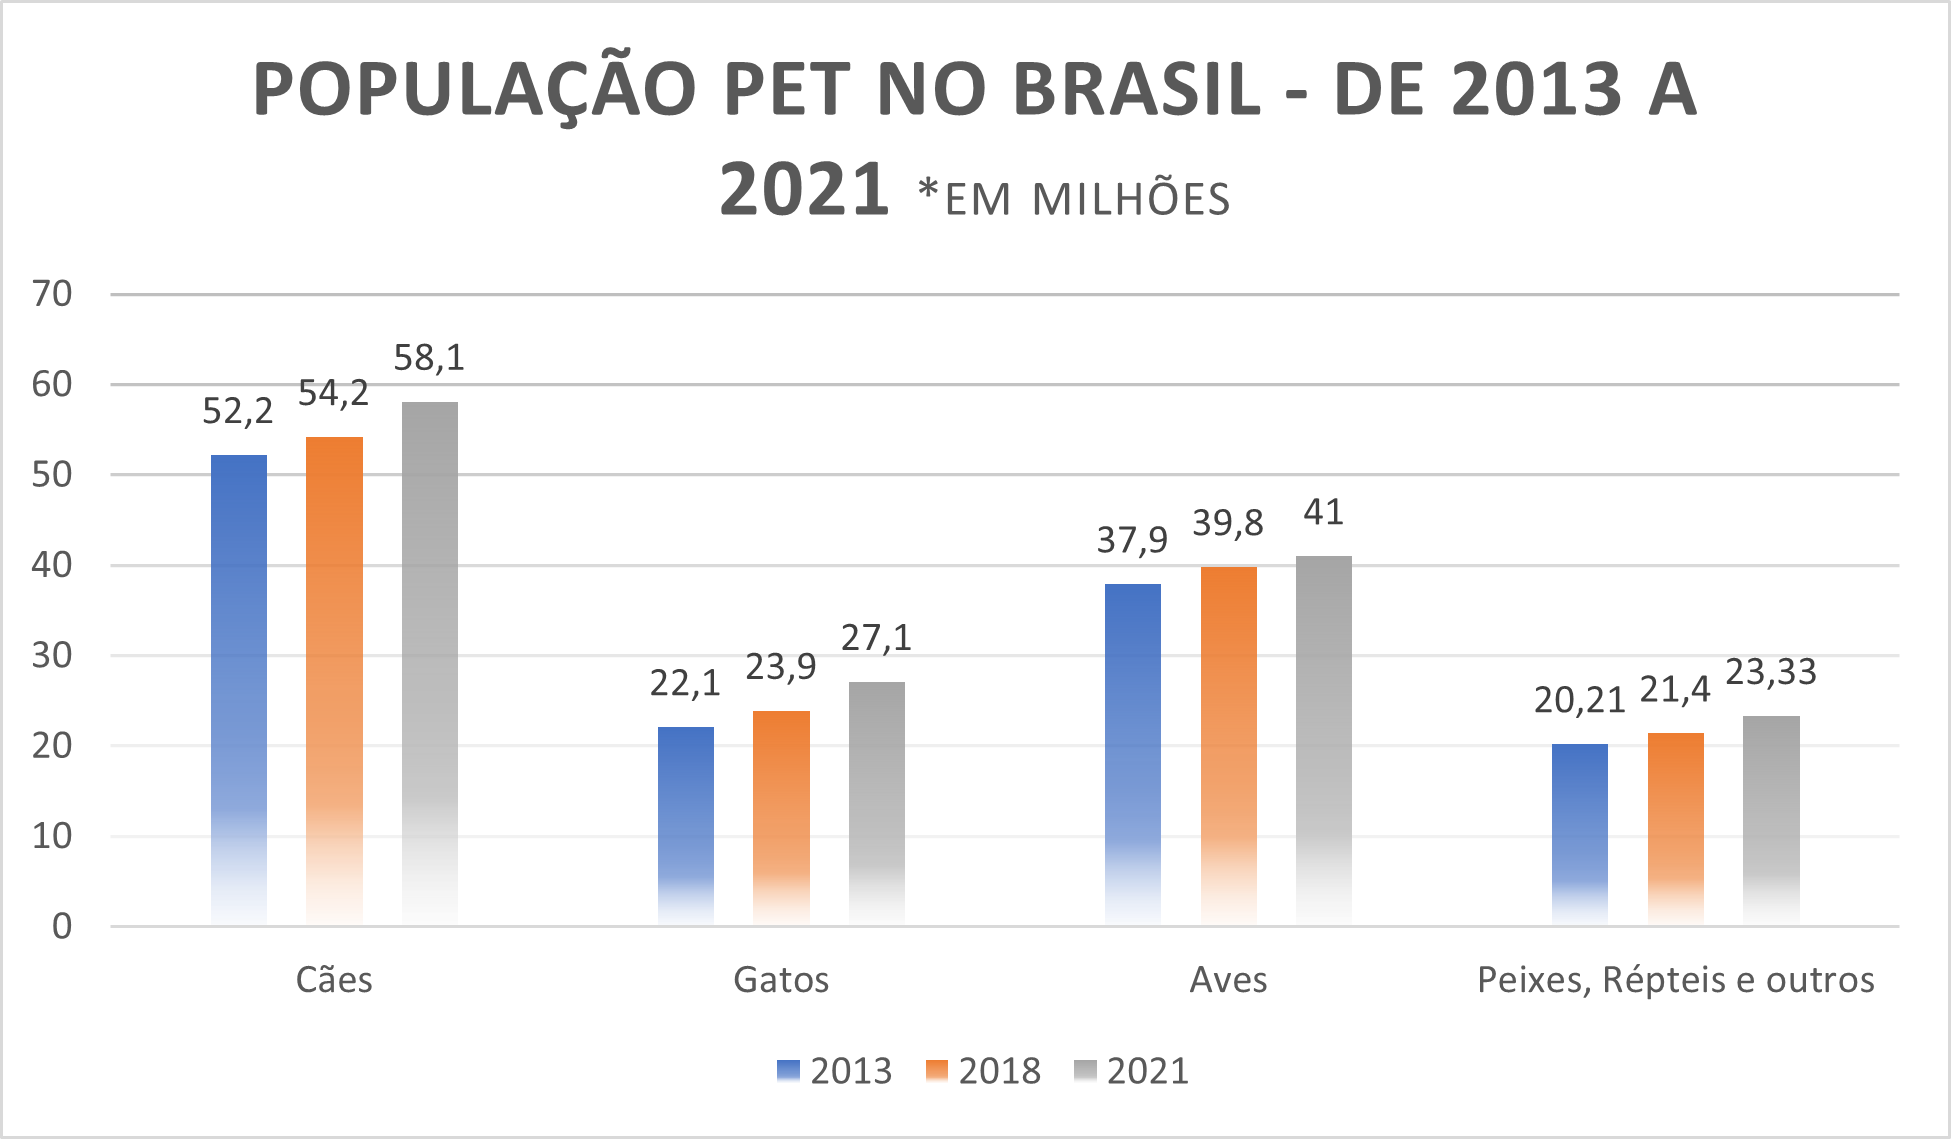
\includegraphics{images/grafico_censopet.png}
        \caption{\DIFaddFL{Censo população Pet no Brasil\mbox{%DIFAUXCMD
\cite{ibge2013, ibge2018, pet2021}}\hskip0pt%DIFAUXCMD
}}
        \label{fig:grafico pet}
    \end{figure}

    \DIFaddend \section{Análise da situação atual}
    \DIFdelbegin \DIFdel{Prontuários veterinários em formato digital }\DIFdelend \DIFaddbegin 

    \DIFadd{O documento obrigatório de maior valor durante o atendimento é, sem dúvidas, o prontuário veterinário. Atualmente }\DIFaddend são \DIFaddbegin \DIFadd{utilizados tanto versões físicas como versões digitais, ou eletrônicas, dos prontuários.
    }

    \DIFadd{Os prontuários eletrônicos são }\DIFaddend oferecidos por diversos sistemas de gerenciamento de clínicas veterinárias, sendo amplamente empregados \DIFdelbegin \DIFdel{como forma de armazenamento de }\DIFdelend \DIFaddbegin \DIFadd{por oferecerem armazenamento com }\DIFaddend acesso fácil aos dados \DIFdelbegin \DIFdel{de }\DIFdelend \DIFaddbegin \DIFadd{dos }\DIFaddend prontuários\DIFdelbegin \DIFdel{de forma segura e confiável. }%DIFDELCMD < 

%DIFDELCMD <     %%%
\DIFdel{Apesar da fidedignidade }\DIFdelend \DIFaddbegin \DIFadd{. Apesar da fidelidade }\DIFaddend das versões virtuais, os dados armazenados não podem \DIFdelbegin \DIFdel{ser utilizadas em substituição aos documentos oficiais }\DIFdelend \DIFaddbegin \DIFadd{substituir documentos físicos }\DIFaddend em eventos judiciais por não serem \DIFdelbegin \DIFdel{aceitos pelo }\DIFdelend \DIFaddbegin \DIFadd{devidamente disciplinados por }\DIFaddend órgão \DIFdelbegin \DIFdel{de classe.
    }\DIFdelend \DIFaddbegin \DIFadd{regulamentador, nesse caso, pelos órgãos de classe que atestem a validade \mbox{%DIFAUXCMD
\cite{pe_dig} }\hskip0pt%DIFAUXCMD
\mbox{%DIFAUXCMD
\cite{prontuario}}\hskip0pt%DIFAUXCMD
.
}\DIFaddend 

    \DIFdelbegin \DIFdel{A gestão de medicamentos controlados (de uso restrito e com retenção de receitas, de acordo com as leis vigentes da INSTRUÇÃO NORMATIVA Nº 35, DE 11 DE SETEMBRO DE 2017, Capítulo I, art 2º, § IV, Capitulo IV, § 11  \mbox{%DIFAUXCMD
\cite{normativa} }\hskip0pt%DIFAUXCMD
é realizada através de um caderno de capa dura, no formato brochura, no qual o médico veterinário responsável técnico (RT) anota a data de entrada dos medicamentos no estoque e quanto desse medicamento foi utilizado no dia, para cada procedimento.
Este caderno é denominado Livro-Registro.
}%DIFDELCMD < 

%DIFDELCMD < %%%
\section{\DIFdel{Problema}}
    %DIFAUXCMD
\addtocounter{section}{-1}%DIFAUXCMD
\DIFdel{Os }\DIFdelend \DIFaddbegin \DIFadd{Além da questão regulatória, os }\DIFaddend sistemas de prontuários digitais \DIFdelbegin \DIFdel{disponíveis atualmente no mercado permitem }\DIFdelend \DIFaddbegin \DIFadd{atualmente disponíveis no mercado não torna os documentos imutáveis ou registram histórico de modificações. Assim, ao permitirem }\DIFaddend a alteração dos dados inseridos, \DIFdelbegin \DIFdel{sem garantir uma forma de }\DIFdelend \DIFaddbegin \DIFadd{não permitirem }\DIFaddend consultar o histórico \DIFdelbegin \DIFdel{destas }\DIFdelend \DIFaddbegin \DIFadd{de alterações }\DIFaddend ou meios de rastreá-las, \DIFaddbegin \DIFadd{sujeita o estabelecimento ao risco desamparo }\DIFaddend em caso de fiscalização por órgãos públicos ou perícias judiciais.
    \DIFaddbegin 

    \DIFaddend Haja vista a \DIFdelbegin \DIFdel{premissa de armazenamento dos arquivos, estes são mantidos de forma física utilizando }\DIFdelend \DIFaddbegin \DIFadd{falta de dificuldade dos sistemas atuais de dar apoio em caso de fiscalizações e a premissa da existência de arquivos físicos, torna-se necessário manter os registros físicos em }\DIFaddend pastas-fichários após serem carimbados e assinados pelo médico veterinário \DIFaddbegin \DIFadd{\mbox{%DIFAUXCMD
\cite{pe_dig}}\hskip0pt%DIFAUXCMD
}\DIFaddend .

    O gerenciamento dos medicamentos controlados é \DIFdelbegin \DIFdel{feito }\DIFdelend \DIFaddbegin \DIFadd{realizado através de anotações manuais }\DIFaddend em um livro de registro\DIFdelbegin \DIFdel{por meio de anotações que }\DIFdelend \DIFaddbegin \DIFadd{. Esses registros }\DIFaddend devem ser realizadas periodicamente e \DIFdelbegin \DIFdel{de maneira correta }\DIFdelend \DIFaddbegin \DIFadd{com exatidão }\DIFaddend pelo profissional veterinário, orientando e definindo os procedimentos a serem adotados dentro da clínica, \DIFdelbegin \DIFdel{prevenindo eventuais }\DIFdelend \DIFaddbegin \DIFadd{a fim de prevenir }\DIFaddend descumprimentos das orientações. No entanto, demandam \DIFdelbegin \DIFdel{de mais tempo que o ideal }\DIFdelend \DIFaddbegin \DIFadd{reserva de tempo e atenção }\DIFaddend para a execução de alguns desses procedimentos, como a operação de cálculos manuais para cada valor ou a repetição de anotações de mesmos dados em diferentes documentos, podendo interferir na performance e exigindo mais esforço do profissional \DIFaddbegin \DIFadd{\mbox{%DIFAUXCMD
\cite{normativa}}\hskip0pt%DIFAUXCMD
}\DIFaddend .

    Além das desvantagens supracitadas, o armazenamento desses arquivos ocupa espaço físico e estão sujeitos a danos e perdas por mau armazenamento, como incidentes gerados por umidade, fogo, roubos e etc. O preenchimento desses dados em versões físicas e depois transcritos para versões digitais, pode ser um processo demorado e é sujeito a falhas, demandando um tempo que poderia ser melhor aplicado pelos profissionais envolvidos. Além disso, torna-se necessário um grau elevado de organização por parte da clínica, de tal modo que não prejudique que a consulta aos arquivos seja possível de forma a facilitar o serviço do profissional\DIFaddbegin \DIFadd{\mbox{%DIFAUXCMD
\cite{pe_dig}}\hskip0pt%DIFAUXCMD
}\DIFaddend .

    \section{Objetivos}

    A área de medicina veterinária ainda hoje opera de forma conservadora devido às suas necessidades burocráticas. E\DIFaddbegin \DIFadd{, }\DIFaddend por mais que o mercado ofereça algumas aplicações \DIFdelbegin \DIFdel{a fim }\DIFdelend \DIFaddbegin \DIFadd{que têm a finalidade }\DIFaddend de automatizar o serviço, é difícil encontrar uma opção que ofereça funcionalidades que \DIFdelbegin \DIFdel{cubram de forma completa }\DIFdelend \DIFaddbegin \DIFadd{cumpram completamente }\DIFaddend as necessidades dos profissionais\DIFdelbegin \DIFdel{a fim de sanar todos os problemas listados acima, haja vista que em sua maioria, elas }\DIFdelend \DIFaddbegin \DIFadd{. Um dos motivos é que as soluções }\DIFaddend não são focadas em procedimentos específicos da veterinária, dividindo o \DIFdelbegin \DIFdel{escopo }\DIFdelend \DIFaddbegin \DIFadd{ferramenta }\DIFaddend da aplicação com a \DIFdelbegin \DIFdel{área }\DIFdelend \DIFaddbegin \DIFadd{gestão }\DIFaddend de Pet Shop.

    A aplicação, chamada de \DIFdelbegin \DIFdel{Sidekick}\DIFdelend \DIFaddbegin \DIFadd{CertVet}\DIFaddend , tem como objetivo cobrir as principais necessidades de atuação do médico veterinário, automatizando os processos operacionais de atendimento e documentações clínicas, que hoje ainda demandam esforços manuais, \DIFdelbegin \DIFdel{de forma legal e que otimize o }\DIFdelend \DIFaddbegin \DIFadd{cumprimento de normas legais e regulamentares e proponha um }\DIFaddend fluxo do trabalho \DIFaddbegin \DIFadd{eficiente}\DIFaddend , diminuindo o tempo gasto neste, a fim de melhorar o desempenho do profissional, do atendimento e consequentemente da clínica.


    \section{Justificativa}

    \DIFaddbegin \DIFadd{Assim como o número de animais de companhia cresce a cada ano, a quantidade de profissionais veterinários atuantes no mercado brasileiro também apresenta crescimento, com 164.549 médicos veterinários inscritos de acordo com a contabilização do órgão federal, indicado na figura \ref{fig:grafico vet} \mbox{%DIFAUXCMD
\cite{vets_SP, vets2020, vets2022}}\hskip0pt%DIFAUXCMD
.
    }

    \begin{figure}[H]
        \centering
        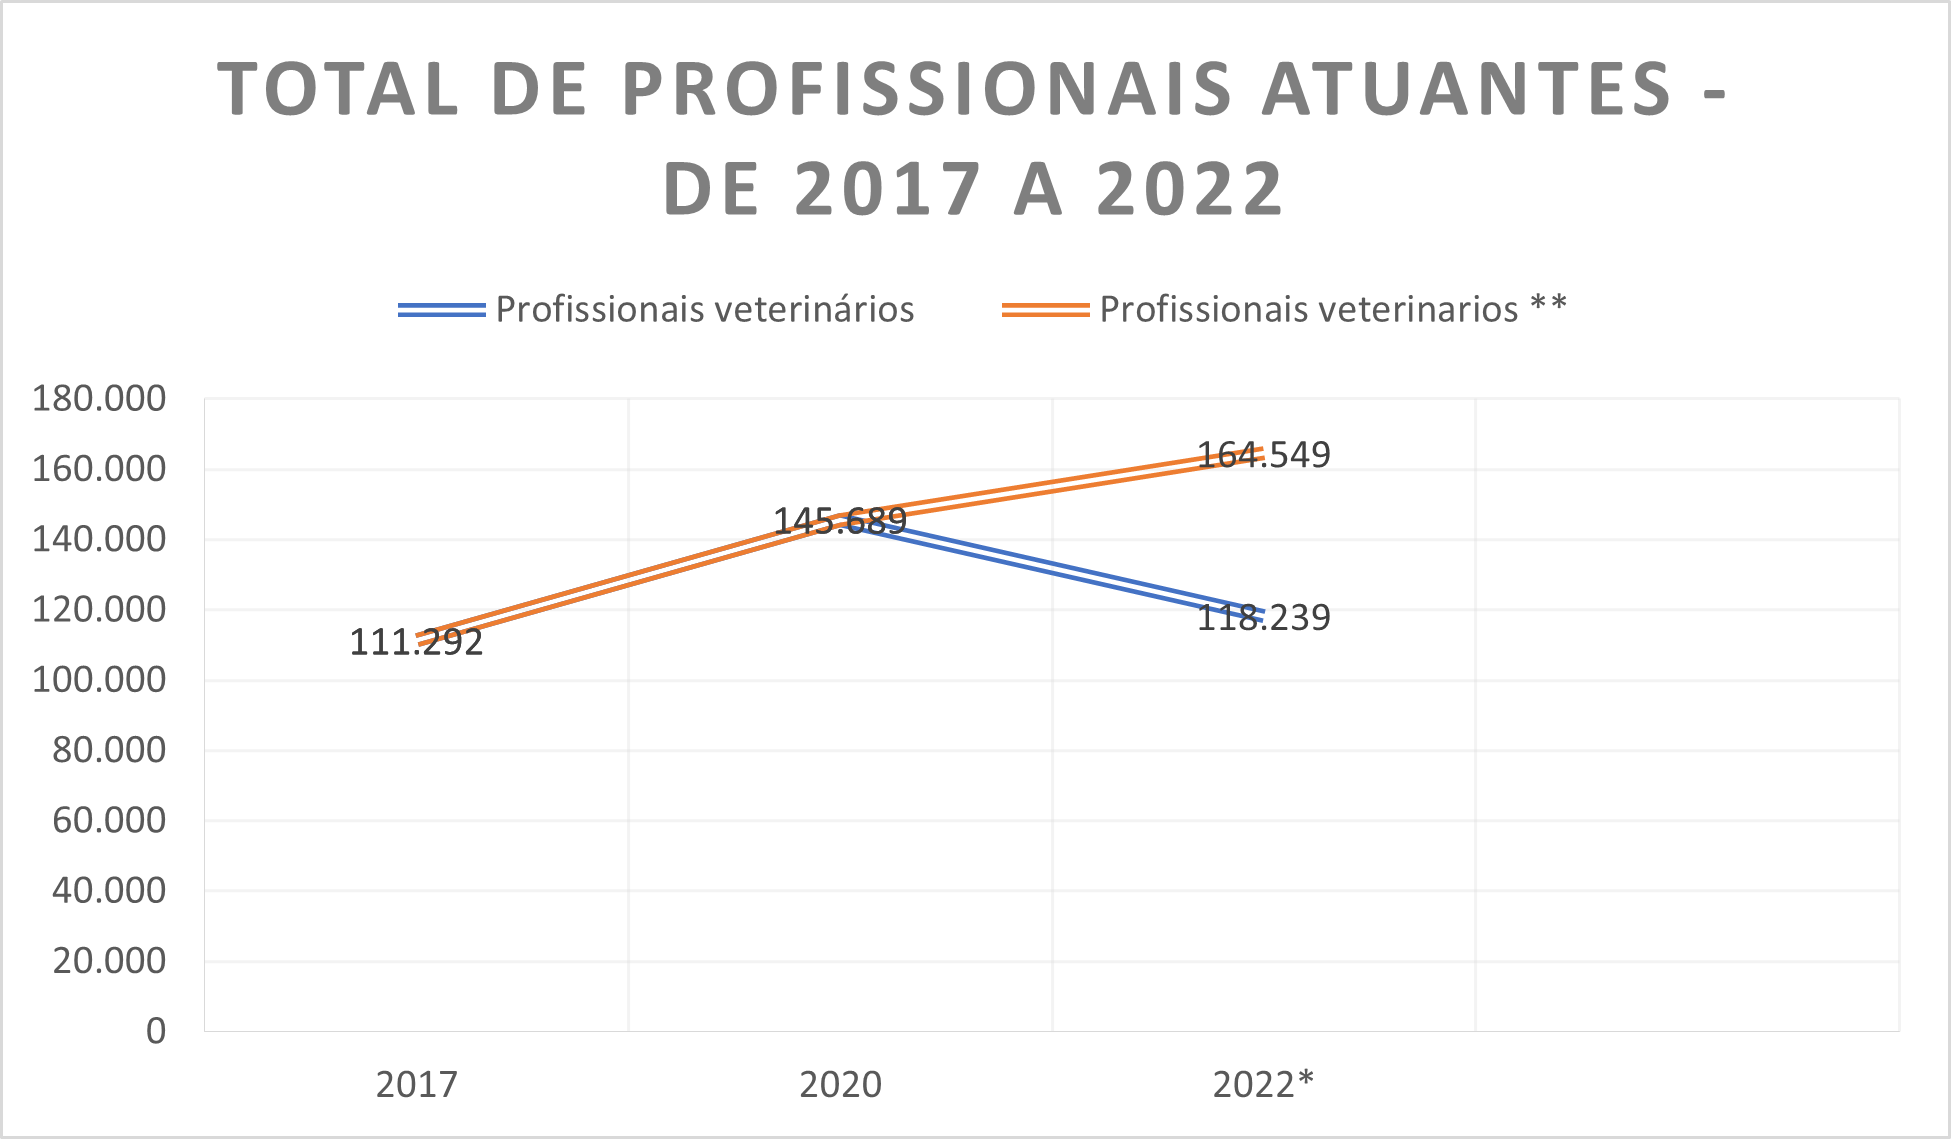
\includegraphics{images/grafico_profissionais.png}
        \caption{\DIFaddFL{*Dados sem contabilizar os inscritos em SP; ** dados incluindo os inscritos em SP\mbox{%DIFAUXCMD
\cite{vets2020,vets2022} }\hskip0pt%DIFAUXCMD
}}
        \label{fig:grafico vet}
    \end{figure}

    \DIFadd{De acordo com o último censo divulgado pelo CFMV (biênio 2021/2022), atualmente existem 46.947 registros ativos de estabelecimentos veterinários, sendo divididos entre clínicas, hospitais, consultórios e ambulatórios, como podemos ver na figura \ref{fig:grafico clinicas} \mbox{%DIFAUXCMD
\cite{clinicas2022}
    }\hskip0pt%DIFAUXCMD
}

    \begin{figure}[H]
        \centering
        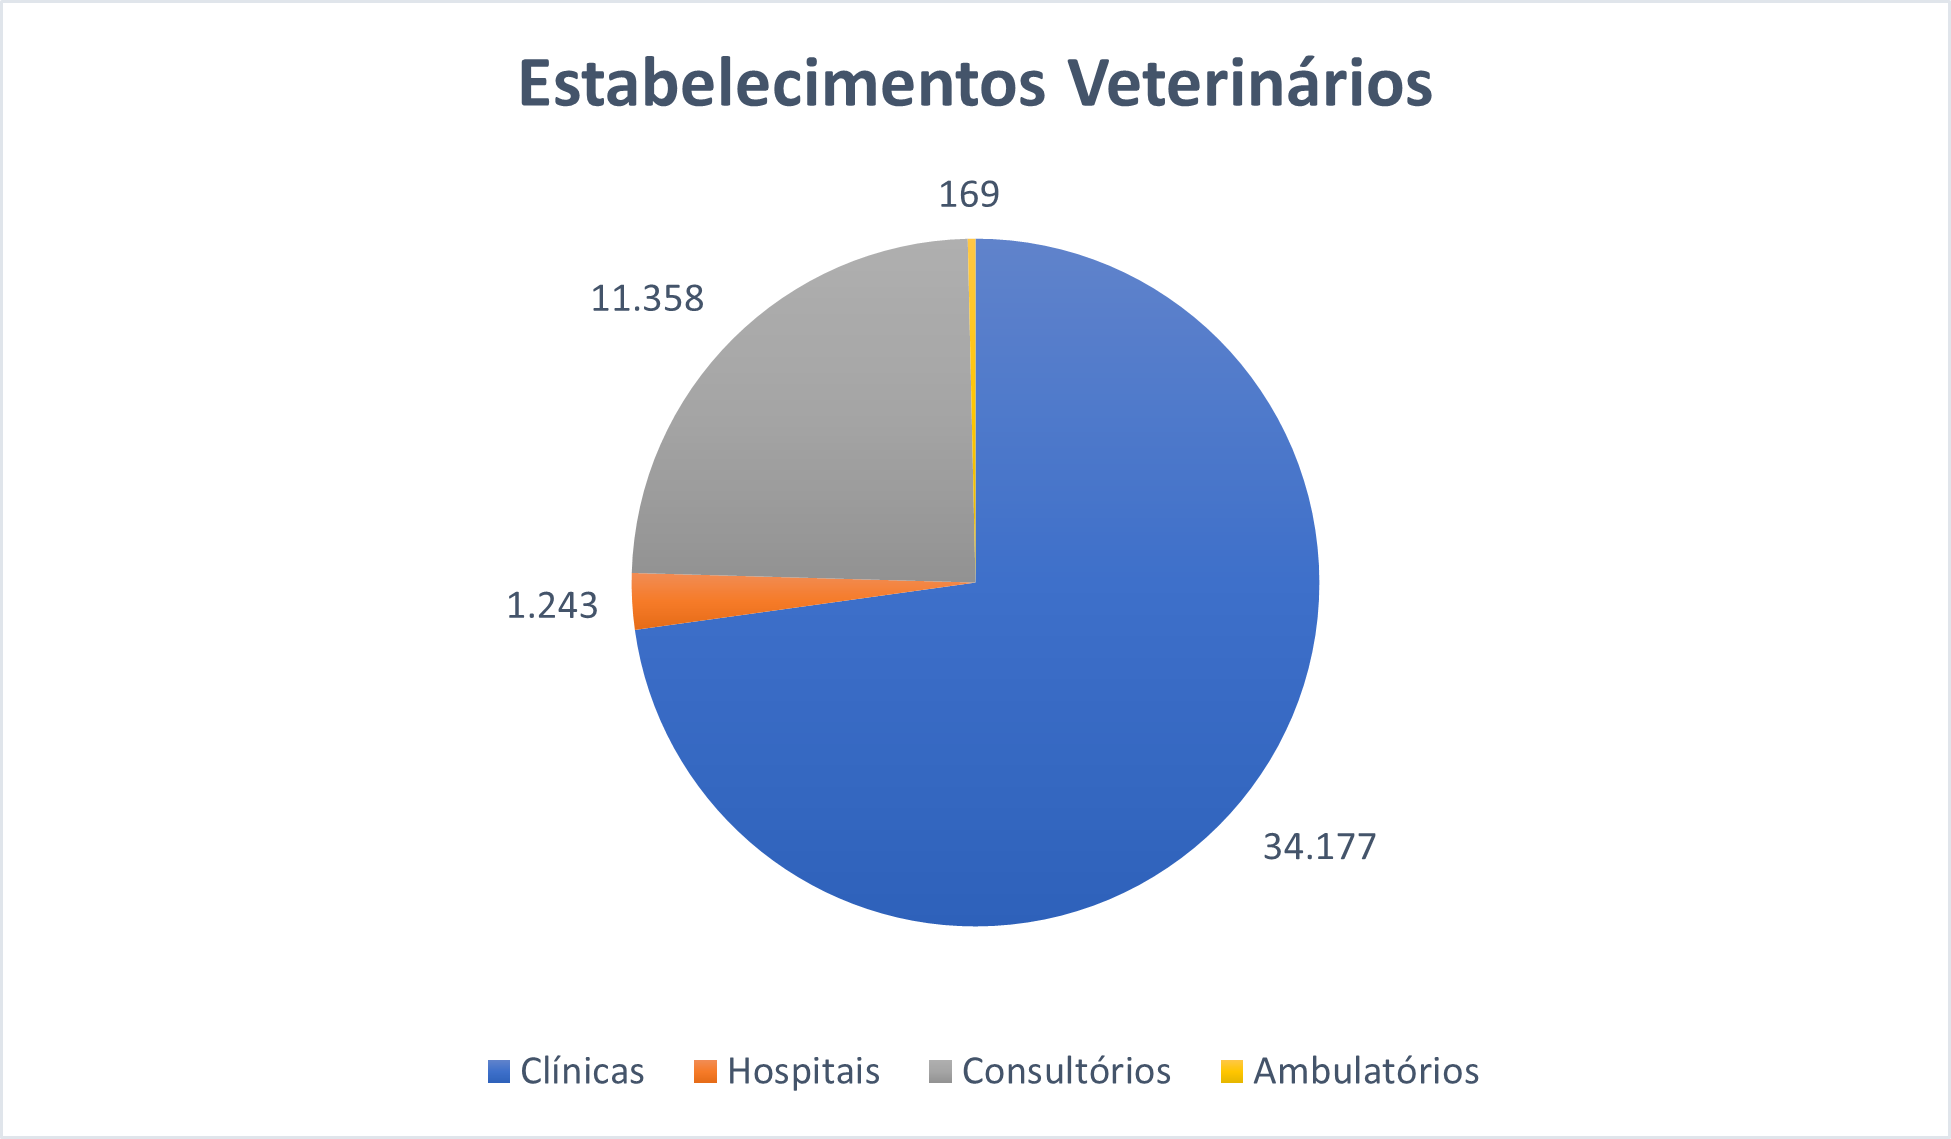
\includegraphics{images/grafico_estabelecimento.png}
        \caption{\DIFaddFL{Censo estabelecimentos veterinários no biênio 2021/2022\mbox{%DIFAUXCMD
\cite{clinicas2022}}\hskip0pt%DIFAUXCMD
}}
        \label{fig:grafico clinicas}
    \end{figure}

    \DIFadd{Todos esses profissionais e estabelecimentos são fiscalizados e disciplinado pelas regras de conduta dos sistemas CFMV/CRMVs.
    }

    \DIFaddend Visando oferecer funcionalidades que permitam uma dinamização de todo o fluxo de trabalho do profissional veterinário, \DIFdelbegin \DIFdel{de forma a }\DIFdelend reduzir o tempo gasto com operações manuais, evitar \DIFaddbegin \DIFadd{a necessidades de }\DIFaddend anotações de informações \DIFdelbegin \DIFdel{repetidas e }\DIFdelend \DIFaddbegin \DIFadd{repetidamente e reduzir o risco de }\DIFaddend erros de transcrição nas documentações, a \DIFdelbegin \DIFdel{Sidekick }\DIFdelend \DIFaddbegin \DIFadd{CertVet }\DIFaddend consiste em um sistema que gerencia \DIFdelbegin \DIFdel{, com valor legal, os processos e documentos }\DIFdelend \DIFaddbegin \DIFadd{documentos com potencial valor legal e seus processos processos }\DIFaddend que se fazem necessários no fluxo de trabalho da medicina veterinária\DIFdelbegin \DIFdel{, de forma que permita a fiscalização e rastreabilidade das }\DIFdelend \DIFaddbegin \DIFadd{.
    }

    \DIFadd{Os processos automatizados agilizam os procedimentos fiscalizatórios e permitem que as }\DIFaddend alterações feitas \DIFaddbegin \DIFadd{sejam rastreadas}\DIFaddend , como é \DIFdelbegin \DIFdel{solicitado }\DIFdelend \DIFaddbegin \DIFadd{exigida }\DIFaddend pelo CFMV (Conselho Federal de Medicina Veterinária) e pelo CRMVs (Conselho Regional de Medicina Veterinária)\DIFdelbegin \DIFdel{. }\DIFdelend \DIFaddbegin \DIFadd{\mbox{%DIFAUXCMD
\cite{teleMV}}\hskip0pt%DIFAUXCMD
.
    }

    \DIFaddend A tecnologia da informação está modernizando a rotina de trabalho \DIFdelbegin \DIFdel{das mais diversas }\DIFdelend \DIFaddbegin \DIFadd{em }\DIFaddend áreas \DIFdelbegin \DIFdel{, se faz necessário que as coisas transcorram em um }\DIFdelend \DIFaddbegin \DIFadd{como automações de escritório, farmacêuticas e na medicina humana em estágios bem mais avançados que em relação ao atualmente aplicado na medicina veterinária. Entendemos que existe a oportunidade de propor }\DIFaddend ritmo mais acelerado sem impedir a legalidade dos processos dentro de uma clínica veterinária\DIFdelbegin \DIFdel{, pensando nisso, a }\DIFdelend \DIFaddbegin \DIFadd{.
    }

    \DIFadd{A partir das verificações de ambiente, referencial regulatório e constatação da situação, verificamos que o desenvolvimento de uma }\DIFaddend aplicação \DIFdelbegin \DIFdel{é pautada pela }\DIFdelend \DIFaddbegin \DIFadd{focada na }\DIFaddend automação de processos operacionais \DIFdelbegin \DIFdel{, }\DIFdelend \DIFaddbegin \DIFadd{que }\DIFaddend otimizando o tempo \DIFdelbegin \DIFdel{da }\DIFdelend \DIFaddbegin \DIFadd{de }\DIFaddend execução das tarefas do profissional veterinário \DIFaddbegin \DIFadd{e confiabilidade dos registros inseridos}\DIFaddend .

    \DIFdelbegin \chapter[Projeto]{\DIFdel{Projeto}}
%DIFAUXCMD
\addtocounter{chapter}{-1}%DIFAUXCMD
\DIFdel{O projeto }\DIFdelend \DIFaddbegin \DIFadd{Em pesquisa bibliográfica, não foram identificados fatos referentes a quantidade de profissionais ou estabelecimentos que utilizam algum sistema eletrônico ou de gestão. Porém, os meios de comunicação comumente enfatizam o crescimento de relevância econômica de serviços para o mercado de animais de estimação ano a ano. O sistema CertVet tem potencial para crescer e se destacar entre os demais sistemas já existentes.
    }


\chapter{\DIFadd{Revisão da Literatura}}

    \DIFadd{Este capítulo abordará uma breve revisão bibliográfica sobre a documentação obrigatória emitida por estabelecimentos veterinários, revisão das leis referentes a tais documentos, novos caminhos abordados pelo Conselho Federal de Medicina Veterinária e como esse aspectos são relevantes ao nosso projeto.
}


    \section{\DIFadd{Documentação Obrigatória e Legislação Pertinente}}

        \DIFadd{De acordo com a Resolução nº1321, de 24 de abril de 2020 \mbox{%DIFAUXCMD
\cite }\hskip0pt%DIFAUXCMD
}{\DIFadd{doc_obrig}}\DIFadd{, todo estabelecimento veterinário e/ou médico veterinário deve emitir documentos específicos no âmbito de suas respectivas atividades profissionais.
        }

        \DIFadd{Tais documentos, de caráter obrigatório, deve seguir os padrões estabelecidos pelo Conselho Federal de Medicina Veterinária, que regulamenta a profissão do médico veterinário, de acordo com a Lei nº 5.517, alínea “f”, do artigo 16, de 23 de outubro de 1968. \mbox{%DIFAUXCMD
\cite }\hskip0pt%DIFAUXCMD
}{\DIFadd{doc_obrig}}\DIFadd{.
        }

        \DIFadd{A Resolução 1321/2020, em seu Art. 2º, define o prontuário veterinário como \mbox{%DIFAUXCMD
\cite }\hskip0pt%DIFAUXCMD
}{\DIFadd{doc_obrig}}\DIFadd{: 
    }

        \begin{quote}
            \DIFadd{VIII - prontuário médico-veterinário: documento escrito e datado, sem rasuras ou emendas, emitido e assinado, privativamente por médico-veterinário que relata e detalha, cronologicamente, informações e dados acerca dos atendimentos ambulatoriais e clínicos, inclusive vacinações, exames diagnósticos e intervenções cirúrgicas realizados em animal, ou coletivo em se tratando de rebanho, garantida a autenticidade e integridade das informações;
        }\end{quote}

        \DIFadd{Outros documentos obrigatórios são \mbox{%DIFAUXCMD
\cite{doc_obrig}}\hskip0pt%DIFAUXCMD
.: 
    }

        \begin{itemize}
            \item
            \DIFadd{Atestado ou declaração de óbito,
            }\item
            \DIFadd{Atestado ou declaração de vacinação,
            }\item
            \DIFadd{Atestado sanitário,
            }\item
            \DIFadd{Prontuário médico-veterinário,
            }\item
            \DIFadd{Termo de consentimento livre esclarecido para realização de exames, 
            }\item
            \DIFadd{Termo de consentimento livre esclarecido para realização de procedimentos terapêuticos de risco ou experimental, 
            }\item
            \DIFadd{Termo de consentimento livre esclarecido para retirada de corpo de animal em óbito, 
            }\item
            \DIFadd{Termo de consentimento livre esclarecido para realização de procedimento cirúrgico, 
            }\item
            \DIFadd{Termo de consentimento livre esclarecido para realização de procedimento anestésico, 
            }\item
            \DIFadd{Termo de consentimento livre esclarecido para internação e tratamento clínico ou pós-cirúrgico, 
            }\item
            \DIFadd{Termo de consentimento livre esclarecido para realização de eutanásia, 
            }\item
            \DIFadd{Termo de consentimento livre esclarecido para retirada do serviço veterinário sem alta médica, 
            }\item
            \DIFadd{Termo de consentimento livre esclarecido para doação de corpo de animal para ensino e pesquisa, 
            }\item
            \DIFadd{Termo de consentimento livre esclarecido para realização de pesquisa clínica.
        }\end{itemize}

        \DIFadd{Dentre as regras referidas na resolução nº 1321 de 2020, seu artigo 3º disciplina dados para a composição do prontuário médico:
    }

        \begin{quote}
            \DIFadd{Os documentos emitidos por médicos-veterinários comporão o prontuário do paciente (...) conter os seguintes dados e informações: nome completo e assinatura do médico-veterinário, número de inscrição no Sistema CFMV/CRMVs, endereço, telefone, e-mail e, se for o caso, identificação do estabelecimento (razão social, CNPJ e número de registro no Sistema CFMV/CRMVs)
        }\end{quote}

        \DIFadd{No inciso VI, especifica fatos relacionados ao animais que devem constar por observação física:
        }

        \begin{quote}
            \DIFadd{(Deve) conter informações que permitam a identificação do paciente, tais como nome, sexo, raça, idade real ou presumida, cor de pelagem ou plumagem, sinais particulares, tatuagem, brinco, microchip, registro genealógico e, conforme o caso, resenha detalhada;(...) identificação do responsável pelo animal (nome completo, CPF e endereço completo)
        }\end{quote}

        \DIFadd{Em seu inciso VII, § 2º, dispõe sobre requisitos para operação de através de mídias virtuais: 
    }

        \begin{quote}
            \DIFadd{Os documentos expedidos eletronicamente deverão contar com sistemas capazes de garantir a segurança, autenticidade, confidencialidade e integridade de informações, bem como o armazenamento e compartilhamento dos dados.
        }\end{quote}

        \DIFadd{Tais regulamentações garantem a legitimidade do sistema proposto pela equipe Rocket, sendo embasamento legal e diretrizes a serem seguidas.
        }

        \DIFadd{A autorização para se realizar a telemedicina na área veterinária também adere à tendência de modernização na profissão e viabiliza que soluções digitais sejam implementadas relativas a documentação obrigatória.\mbox{%DIFAUXCMD
\cite{teleMV}}\hskip0pt%DIFAUXCMD
.
        }

        \DIFadd{Com relação a gestão de medicamentos controlados (de uso restrito e com retenção de receitas), de acordo com as leis vigentes da INSTRUÇÃO NORMATIVA Nº 35, DE 11 DE SETEMBRO DE 2017, Capítulo I, Art. 2º, § IV, Capitulo IV, § 11  \mbox{%DIFAUXCMD
\cite{normativa}}\hskip0pt%DIFAUXCMD
, ela é realizada através de um caderno de capa dura, no formato brochura, no qual o médico veterinário responsável técnico (RT) anota a data de entrada dos medicamentos no estoque e quanto desse medicamento foi utilizado no dia, para cada procedimento. Este caderno é denominado Livro-Registro.
}


\chapter[Metodologias]{\DIFadd{Metodologias}}

    \DIFadd{O projeto }\DIFaddend propõe a criação de um sistema de gerenciamento de processos e documentação exigidas pelo órgão de classe veterinária, além de \DIFdelbegin \DIFdel{agregar funcionalidades }\DIFdelend \DIFaddbegin \DIFadd{implementar funcionalidades já }\DIFaddend existentes em outros sistemas de \DIFdelbegin \DIFdel{gerenciamento }\DIFdelend \DIFaddbegin \DIFadd{gestão }\DIFaddend de estabelecimentos veterinários. 

    \section{Proposta}
    \DIFdelbegin \DIFdel{Uma }\DIFdelend \DIFaddbegin 

        \DIFadd{A }\DIFaddend solução \DIFdelbegin \DIFdel{seria criar arquivos que tivessem }\DIFdelend \DIFaddbegin \DIFadd{inicial aplica a assinatura eletrônica aos arquivos gerados a partir da aplicação, utilizando }\DIFaddend um certificado digital \DIFdelbegin \DIFdel{, ou similar, para a verificação }\DIFdelend \DIFaddbegin \DIFadd{válido padrão ICP-Brasil. Este processo garante a verificabilidade }\DIFaddend e rastreabilidade de alterações feitas, \DIFdelbegin \DIFdel{com }\DIFdelend \DIFaddbegin \DIFadd{bem como os devidos registros de }\DIFaddend data e hora\DIFdelbegin \DIFdel{das alterações}\DIFdelend , sendo assim, passível de fiscalização.
        \DIFdelbegin \DIFdel{Outra solução seria cruzar o banco de dados dos medicamentos controlados}\DIFdelend \DIFaddbegin 

        \DIFadd{Complementarmente, para os registros de medicamentos controlados, é possível cruzar os dados movimentação de determinados medicamentos }\DIFaddend disponíveis no estoque, \DIFdelbegin \DIFdel{e registrados }\DIFdelend \DIFaddbegin \DIFadd{suas movimentações }\DIFaddend no livro-registro \DIFdelbegin \DIFdel{, com os }\DIFdelend \DIFaddbegin \DIFadd{e }\DIFaddend valores desses medicamentos que estão sendo utilizados durante os procedimentos, \DIFdelbegin \DIFdel{evitando-se assim que o médico veterinário tenha que anotar, a mão, várias vezes o mesmo dado. O próprio sistema ficará responsável pelos }\DIFdelend \DIFaddbegin \DIFadd{atribuindo maior consistência aos registros e diminuindo o retrabalho de se adicionar as mesmas informações manualmente. O sistema realiza os }\DIFaddend cálculos \DIFdelbegin \DIFdel{da }\DIFdelend \DIFaddbegin \DIFadd{de }\DIFaddend quantidade de medicamentos utilizados e atualizar no livro-registro digital.

    \section{Funcionalidades}
    \DIFaddbegin 

        \DIFadd{A partir do entendimento da concorrência e entendimento do dia a dia de uma clínica veterinária, serão implementadas as seguintes funcionalidades:
    }

        \DIFaddend \begin{itemize}
            \item Cadastro de funcionários, clientes, animais e atendimentos.
            \item Assinatura digital, ou similar, para rastrear e verificar alterações feitas no prontuário.
            \item Validador de cadastro profissional para acessar área restrita do sistema.
            \item Cruzamento de dados entre medicamentos utilizados e inseridos no Estoque.
            \item Mapeamento Genealógico do animal.
        \end{itemize}

        \subsection{Funcionalidades Futuras}
            \DIFaddbegin 

            \DIFaddend Algumas possíveis implementações de funcionalidades futuras são a criptografia do dados, importação e exportação dos dados entre estabelecimentos que utilizam o mesmo sistema, digitalização das notificações de aquisição de medicamentos controlados com a nota fiscal da compra do produto, automatizando a entrada desses dados no estoque e permitindo a fiscalização.

        \subsection{\DIFdelbegin \DIFdel{Histórias de Usuários}\DIFdelend \DIFaddbegin \DIFadd{Possíveis Integrações e Parcerias}\DIFaddend }

            \DIFdelbegin %DIFDELCMD < \begin{enumerate}
%DIFDELCMD <     %%%
\DIFdelend \DIFaddbegin \DIFadd{O sistema CertVet deverá se integrar ao SISCAD (Sistemas de Cadastros do Conselho Federal de Medicina Veterinária) para validar o registros de profissionais ativos e sendo registrados na plataforma.
            }

            \DIFadd{Uma possível parceria seria os próprios órgãos de fiscalização regional de cada Estado, CRMVs.
    }

    \section{\DIFadd{Análise de Concorrência}}

        \DIFadd{Nos últimos anos ocorreu modernização na dinâmica que rege a profissão do médico veterinário tanto pelo conselho federal, como por seus órgãos regionais \mbox{%DIFAUXCMD
\cite{art_digital} }\hskip0pt%DIFAUXCMD
\mbox{%DIFAUXCMD
\cite{cart_digital} }\hskip0pt%DIFAUXCMD
possibilitando que documentos obrigatoriamente físicos pudessem ser registrados em versões digitais válidos em todo território nacional. 
        }

        \DIFadd{A solicitação de tais documentos também podem ser realizados via navegação humana por sistema web disponibilizado publicamente pelo CFMV, utilizando meios de identificação e autenticação nos sistemas regentes \mbox{%DIFAUXCMD
\cite{art_digital}}\hskip0pt%DIFAUXCMD
.
        }

        \DIFadd{Este mesmo dado também pode ser utilizado por interface de aplicação, uma vez liberado por usuário habilitado por intermédio do CFMV.
    }

        \DIFadd{Para fins de comparação, foram selecionadas as principais aplicações já presentes no mercado que atuam na mesma problemática da CertVet.
}

\subsection{\DIFadd{Tabela comparativa}}
\begin{center}
    \begin{table}[H]
    \begin{tabulary}{1.0\textwidth}{|L|L|L|L|L|L|L|L|L|}
    \hline
     & \DIFaddFL{CertVet }& \DIFaddFL{Simples Vet }& \DIFaddFL{Vet work }& \DIFaddFL{Doctor Vet }& \DIFaddFL{Dr. Snoopy Smart }& \DIFaddFL{Vet soft }& \DIFaddFL{Beans Vet}\\
    \hline
    \DIFaddFL{Agenda }& \DIFaddFL{x }& \DIFaddFL{x }& \DIFaddFL{x }& \DIFaddFL{x }& \DIFaddFL{x }& \DIFaddFL{x }& \DIFaddFL{x}\\
    \hline
    \DIFaddFL{Prontuário clínico }& \DIFaddFL{x }& \DIFaddFL{x }& \DIFaddFL{x }& \DIFaddFL{x }& \DIFaddFL{x }& \DIFaddFL{x }& \DIFaddFL{x}\\
    \hline
    \DIFaddFL{Gerenciamento de medicação }& \DIFaddFL{x }& \DIFaddFL{x }&  & \DIFaddFL{x }& \DIFaddFL{x }& \DIFaddFL{x }& \DIFaddFL{x}\\
    \hline
    \DIFaddFL{Controle de vacina\c{c}ão }& \DIFaddFL{x }&  &  & \DIFaddFL{x }& \DIFaddFL{x }& \DIFaddFL{x }& \DIFaddFL{x}\\
    \hline
    \DIFaddFL{Mapeamento genealógico }& \DIFaddFL{x }&  &  &  &  &  & \\
    \hline
    \DIFaddFL{Rastreio de alterações }& \DIFaddFL{x }&  &  &  &  &  & \\
    \hline
    \end{tabulary}
    \caption{\DIFaddFL{Análise Comparativa}}
    \label{tab:comparativa}
    \end{table}
\end{center}

\subsection{\DIFadd{SimplesVet}}
\DIFadd{O SimplesVet se apresenta como um sistema para petshop e clínica veterinária que busca ajudar a simplificar a rotina da clínica. Consiste em um sistema acessado via WEB, permitindo o controle da clínica a qualquer hora ou lugar, contanto que tenha acesso a internet. Suas funcionalidades dividem-se em:
}

\begin{itemize}

    \DIFaddend \item \DIFaddbegin \DIFadd{Atendimento veterinário: permite o registro das fichas veterinárias em uma tela simples, com dados salvos na nuvem.
    }\item \DIFadd{Agenda de serviços: possibilita a organização da agenda dos veterinários e envia lembretes sobre os próximos atendimentos.
    }\item \DIFadd{Internação veterinária: organização dos prontuários e agendas de plantão.
    }\item \DIFadd{Controle financeiro: possibilita a organização do fluxo de caixa da clínica e envia lembretes de contas a pagar no celular cadastrado.
    }\item \DIFadd{Gestão de estoque: visualização dos produtos a repor, itens próximos ao vencimento, produtos parados e etc.
    }\item \DIFadd{Análise de vendas: visualização de um dashboard voltado à estratégias de marketing, listando produtos mais vendidos, ticket médio, horários de pico e etc.
    }\item \DIFadd{Notas fiscais: emissão de notas fiscais de produto (NFC-e), serviço (NFS-e) e nota grande (NF-e).
    }\item \DIFadd{App para tutores: um app feito para o cliente com datas de vacinação, exames e informações do pet.
    }\item \DIFadd{Mensagens automáticas: envio de lembrete de consultas e vacinas para os tutores e agenda para veterinários.
    }\item \DIFadd{SMS Marketing: envio de campanhas via SMS para os clientes.
    }\item \DIFadd{Pesquisa e satisfação: possibilita o recebimento de avaliações dos clientes para fins comparativos com o mercado.
}\end{itemize}

\DIFadd{A SimplesVet possui mais features voltadas à gerência de assuntos de PetShop, como controle de estoque e de vendas, cumprindo de forma básica apenas uma das demandas da clínica veterinária. Enquanto a Certvet tem como principal objetivo resolver de forma simples as demandas do ambiente clínico, voltadas principalmente ao trabalho realizado pelo veterinário, como: manutenção de prontuário digital, controle de internação, controle da medicação e da autenticação de receitas, dentre outras, resolvendo demandas que não são contempladas pelo SimplesVet.
}

\subsection{\DIFadd{Vetwork}}
\DIFadd{O Vetwork destaca-se entre os usuários pela sua interface intuitiva sendo algo que auxilia na produtividade do trabalho, trata-se de um sistema de gestão baseado na nuvem, não fazendo necessária a instalação de hardware ou software, pois funciona nativo SaaS. Seus 2.744 usuários dispõem das seguintes funcionalidades:
}

\begin{itemize}
    \item \DIFadd{Agenda vinculada ao caixa: um controle geral das atividades realizadas nos pets, como consultas médicas, retornos, exames, cirurgias, banhos, tosas e todos os outros procedimentos, sem limite de datas.
    }\item \DIFadd{Gestão de Documentos: permite a inclusão de documentos e arquivos à ficha clínica do animal, como laudos, fotografias, exames de imagem e outros, que são armazenados na internet e podem ser acessados de qualquer lugar.
    }\item \DIFadd{Calendário: uma forma de controle das datas e horários em que os animais passaram por procedimentos como banhos, tosas, exames, consultas, vacinas ou quaisquer outros realizados no estabelecimento.
    }\item \DIFadd{Gestão clínica: criação de prontuário eletrônico com as informações médicas do pet, como controle de registros clínicos, exames, vacinas e doses adicionais.
    }\item \DIFadd{Gestão Financeira: controle de caixa, pacotes, contas a pagar e a receber, pagamentos pendentes e pré-vendas, cálculo de comissionamento e geração de relatórios financeiros da empresa.
    }\item \DIFadd{Relacionamento com o Cliente: armazenamento de todas as informações dos clientes para possibilitar um relacionamento mais próximo com o mesmo.
    }\item \DIFadd{E-mail Inclusos: mensagens automáticas, através de e-mail, para comunicação instantânea.
}\end{itemize}

\DIFadd{Apesar de ser uma aplicação mais completa em relação à anterior, ainda assim o prontuário eletrônico é o ponto forte desse serviço, no que tange à funcionalidades para o fluxo clínico veterinário. A CertVet busca resolver de forma eficaz e mais completa, o controle de medicamentos, não só o seu cadastro e quantidade em estoque, mas o uso de uma chave de autenticação para receitas e a aplicação dos mesmos. De forma resumida, o Vetwork é sim uma ferramenta bem útil mas a aplicação aqui proposta resolve demandas que não são resolvidas por esse serviço, por mais que suas avaliações no mercado sejam positivas.
}

\subsection{\DIFadd{DoctorVet}}
\DIFadd{O DoctorVet é um sistema totalmente voltado à gestão de clínicas e hospitais veterinários e apresenta duas versões: uma standard com módulos para controle de consultas, vacinas, pequenas cirurgias, assuntos de pet shop e também financeiro. E uma versão enterprise que contempla todos os módulos standard e adicionalmente um controle de internação e hospedagem e concentra informações do centro cirúrgico e laboratório.  Funcionalidades da versão Enterprise do DoctorVet:
}

\begin{itemize}
    \item \DIFadd{Módulo de Cadastro: realiza o cadastro de veterinários, funcionários, animais, clientes e planos de atendimento.
    }\item \DIFadd{Módulo Farmacológico: permite o cadastro de vacinas, vermífugos e o cadastro de procedimentos ou interações medicamentosas.
    }\item \DIFadd{Módulo Atendimento: criação de ficha de atendimento, lista de espera, curadoria de orçamentos, central de   agendamentos e controle de status do veterinário.
    }\item \DIFadd{Módulo Caixa: utilizado pelos atendentes de caixa, controle das formas de recebimento, abertura e fechamento do caixa e manutenção.
    }\item \DIFadd{Módulo Consultório: consultas generalistas e especialistas, histórico de consultas e atendimentos, pedidos de exames, receituários e prontuário eletrônico.
    }\item \DIFadd{Módulo Pet Shop: permite televendas, consulta de preços e relatórios e emissão de cupom fiscal.
    }\item \DIFadd{Módulo Internação Básica/ Avançada: admissão de internação, controle da evolução do quadro clínico, alta veterinária, manter prontuários, cadastro de prescrições.
    }\item \DIFadd{Módulo Estoque: cadastro de fornecedores, cadastro e etiquetação de produtos, gerenciamento de lotes, requisições à farmácia e requisições internas, controle de compras e relatórios.
    }\item \DIFadd{Módulo Exames: controle de exames laboratoriais e seus resultados.
    }\item \DIFadd{Módulo Laboratório: cadastros, central de coleta e composição de exames.
    }\item \DIFadd{Módulo Centro Diagnóstico: preparo para exames e suas composições.
    }\item \DIFadd{Módulo Relatórios: criação de relatórios operacionais, gerenciais e estratégicos (CRM, SPED Fiscal e Pis, Cofins)
    }\item \DIFadd{Módulo Segurança: cadastro de usuários e permissões de acesso de acordo com níveis.
}\end{itemize}

\DIFadd{É a aplicação mais recente das selecionadas e também a mais completa, no entanto, reforça-se aqui que não contempla o controle de medicamentos, oferecido pela Certvet.
}

\subsection{\DIFadd{Dr. Snoopy Smart}}
\DIFadd{O Dr. Snoopy Smart se apresenta como um sistema completo de gestão exclusivo para Pet Shop e clínicas veterinárias, automatizando processos clínicos, na tentativa de agilizar as tarefas e tendo o aumento das vendas como foco do módulo de pet shop. Consiste em um software com as seguintes funcionalidades:
}

\begin{itemize}
    \item \DIFadd{Agendamento otimizado: permitindo o controle de agendamento dos pacientes.
    }\item \DIFadd{Gerenciamento de estoque: visibilidade da quantidade de produtos e quais estão em falta.
    }\item \DIFadd{Prontuário Clínico: possibilita a criação e consulta da ficha veterinária dos animais.
    }\item \DIFadd{Emissão de Notas: emissão de NF-e, NFS-e e Cupons Fiscais.
    }\item \DIFadd{Histórico de Pacientes: arquivação e consulta de informações dos atendimentos. 
    }\item \DIFadd{Vacinas sempre em dia: controle de quando o paciente deve ser vacinado.
    }\item \DIFadd{Agenda de Banho e Tosa: específica para tais, permitindo um maior controle do pet shop.
    }\item \DIFadd{Gestão Integrada: permite acessar à determinados indicadores de gestão.
    }\item \DIFadd{Notificações SMS: recebimento de lembretes importantes no celular dos usuários da aplicação
    }\item \DIFadd{Relatórios Personalizados: geração de relatórios com facilidade.
}\end{itemize}

\DIFadd{Apesar de ser uma aplicação com muitas funcionalidades, ainda assim não apresenta as opções de modernidade que a aplicação aqui proposta oferece, haja vista que divide o escopo clínico com as necessidades de um pet shop, apresentando mais funcionalidades voltadas à gestão e estratégias de venda do que para o fluxo de trabalho do profissional veterinário.
}

\subsection{\DIFadd{Vetsoft}}
\DIFadd{O programa VetSoft é oferecido nas versões Desktop e Web, sendo essa primeira uma versão instalada nos computadores em rede, permitindo o acesso mesmo com falta de conexão com a Internet. E a versão Web, um sistema em nuvem que permite ao usuário gerenciar o negócio através de diferentes dispositivos, como computador, smartphone, tablet, etc, contanto que tenha acesso à Internet. O VetSoft abrange serviços de clínica veterinária, hospital veterinário, pet shop / banho e tosa e veterinários autônomos com as seguintes funcionalidades:
}

\begin{itemize}
    \item \DIFadd{Ficha do Tutor: ficha cadastral da conta do tutor e seus animais, visibilidade do histórico de pagamentos e envio de e-mail individual.
    }\item \DIFadd{Ficha do Animal: ficha cadastral específica dos animais pacientes, álbum de fotos, agendamentos, agrupamento dos resultados de exames e histórico de vacinas e vermífugos.
    }\item \DIFadd{Histórico Clínico: anamnese, diagnóstico, laudo clínico, receituário normal e especial e exames.
    }\item \DIFadd{Gestão de Estoque: divisão de produtos por grupos, controle de produtos com estoque baixo, visibilidade dos produtos mais e menos vendidos e entrada de estoque manual e XML.
    }\item \DIFadd{Financeiro: controle de caixa diário e seu fluxo, demonstrativo de resultados por área, centro de custos, controle de planos para clientes mensalistas.
    }\item \DIFadd{Emissão Fiscal: possibilidade de emissão fiscal para todos os estados e todos os formatos: NFCe, SAT, MFe e PAF-ECF.
    }\item \DIFadd{Farmácia/Materiais: controle de estoque de farmácia e materiais de uso interno.
    }\item \DIFadd{Imunizações: controle da aplicação de vacinas e vermífugos na ficha do animal com agendamentos e aplicações realizadas.
}\end{itemize}

\DIFadd{É uma das aplicações mais completas, no entanto, o controle de medicamentos oferecido não atinge o mesmo grau de segurança que a chave de autenticação para as receitas que a CertVet oferece, assumindo um papel importante na modernização dessa autenticação nos dias atuais.
}

\subsection{\DIFadd{BensVet}}
\DIFadd{O BensVet se diferencia dos demais apresentados por se tratar de um serviço que se divide em dois aplicativos, um para uso veterinário e um para uso dos tutores. O aplicativo para veterinários garante que o usuário poderá iniciar um atendimento a domicílio e conseguir  dar continuidade na clínica. E o aplicativo para tutores trata-se dos processos de envio  de promoções e alertas de retorno automáticos para os tutores, permitindo também a consulta de  informações sobre o animal e agendamento de atendimentos pelo app. As funcionalidades dividem-se em:
}

\begin{itemize}
    \item \DIFadd{Agenda de atendimentos.
    }\item \DIFadd{Acompanhamento de medicações na internação.
    }\item \DIFadd{Criação de fichas clínicas personalizadas.
    }\item \DIFadd{Notificar automaticamente consultas, retornos e vacinas aos clientes.
    }\item \DIFadd{Consultar históricos de animais e seus tutores.
    }\item \DIFadd{Controle dos comissionamentos de profissionais.
    }\item \DIFadd{Emitir Notas Fiscais referente a venda de produtos.
    }\item \DIFadd{Controle de estoque.
}\end{itemize}

\DIFadd{Trata-se de uma resolução que se aproxima bastante da CertVet no que tange à proximidade do profissional veterinário, esteja ele numa clínica ou trabalhando de forma autônoma, no entanto, observamos aqui que o controle de medicamentos oferecido, mais uma vez, não atinge o mesmo grau de segurança que a chave de autenticação aqui propostas, além da funcionalidade de mapeamento genealógico.
}


\postextual

    \section{\DIFadd{Análise de Requisitos}}

        \DIFadd{Na etapa de análise de requisitos, a equipe passa a elaborar em maior nível de detalhamento as regras e características que a aplicação deve suportar, compreendendo de maneira mais assertiva as principais necessidades do cliente e definindo as prioridades do projeto.
        }

        \DIFadd{Esse é um processo evolutivo incremental em que a equipe deve se reunir com o Product Owner em frequência definida a fim de refinar os requisitos levantados para o andamento das histórias registradas como itens do Product Backlog. 
        }

        \DIFadd{Conforme as histórias são desenvolvidas, os membros da equipe criarão tarefas de acordo com o entendimento do refinamento discutido.
        }

        \DIFadd{Partindo das regras de negócio, são apresentados os requisitos funcionais, não funcionais e, por fim, as histórias de usuário.
}

        \subsection{\DIFadd{Regras de Negócio}}

            \DIFadd{As regras de negócio são as premissas necessárias para a modelagem do projeto e através delas serão definidas as regras básicas as quais o sistema deve concernir.
            }

            \DIFadd{Tem por objetivo explicitar as restrições a serem adotadas pelo sistema a fim de garantir assertividade ao escopo definido para completude das ferramentas e histórias em desenvolvimento, bem como as interdependências entre as ferramentas e histõrias relacionadas.
            }

            \DIFadd{O Quadro a seguir dispõe das informações referente às regras de negócios do CertVet:
}

            \begin{center}
                \begin{table}[H]
                \begin{tabulary}{1.0\textwidth}{|C|p{23em}|C|}
                \hline
                 \DIFaddFL{Código }& \DIFaddFL{Descrição }& \DIFaddFL{Requisito Relacionado}\\
                \hline
                \DIFaddFL{RN01 }& \DIFaddFL{Somente após efetuar cadastro contendo todas as informações obrigatórias, o usuário obterá acesso ao sistema. }& \DIFaddFL{RF01}\\
                \hline
                \DIFaddFL{RN02 }& \DIFaddFL{O usuário deve se autenticar informando seu e-mail e senha de cadastro. }& \DIFaddFL{RF02}\\
                \hline
                \DIFaddFL{RN03 }& \DIFaddFL{O usuário terá acesso às funcionalidades de acordo com o seu tipo de conta. }& \\
                \hline
                \DIFaddFL{RN04 }& \DIFaddFL{Apenas profissionais com número de CRMV válido devem ter acesso às funcionalidades clínicas. }& \\
                \hline
                \DIFaddFL{RN05 }& \DIFaddFL{Os prontuários digitais devem seguir o padrão dos modelos oficiais. }& \DIFaddFL{RF10}\\
                \hline
                \DIFaddFL{RN06 }& \DIFaddFL{Somente usuários com autorização podem realizar edições nos prontuários. }& \DIFaddFL{RF11}\\
                \hline
                \DIFaddFL{RN07 }& \DIFaddFL{Na gestão de medicamentos, a retirada deve ser feita apenas por profissionais veterinários autorizados. }& \DIFaddFL{RF14 e RF15}\\
                \hline
                \DIFaddFL{RN08 }& \DIFaddFL{O controle de vacinação deve ser visível por todas as partes envolvidas, profissionais e tutores. }& \DIFaddFL{RF16, RF17 e RF18}\\
                \hline
                \end{tabulary}   \caption{\DIFaddFL{Regra de Negócio}}
                \label{tab:regra}
                \end{table}
            \end{center}

        \subsection{\DIFadd{Requisitos Funcionais}}

            \DIFadd{No Quadro abaixo são apresentados os requisitos funcionais, detalhando as necessidades e especificações das ações que o sistema deve executar, ignorando as limitações físicas, focando apenas no comportamento de entrada e saída do sistema.
            }

            \begin{center}
                \begin{table}[h]
                \centering
                \begin{tabulary}{1.0\textwidth}{|p{5em}|p{8em}|p{18em}|}
                \hline
                \DIFaddFL{Código }& \DIFaddFL{Requisito }& \DIFaddFL{Descrição}\\
                \hline
                \DIFaddFL{RF01 }& \DIFaddFL{Criar conta }& \DIFaddFL{O usuário deve criar uma conta de acordo com a sua ocupação (Veterinário | Auxiliar) e seus dados.}\\
                \hline
                \DIFaddFL{RF02 }& \DIFaddFL{Autenticar usuário }& \DIFaddFL{O sistema deve permitir que o usuário entre em sua conta já criada no sistema.}\\
                \hline
                \DIFaddFL{RF03 }& \DIFaddFL{Alterar senha }& \DIFaddFL{O sistema deve permitir que o usuário altere a sua senha.}\\
                \hline
                \DIFaddFL{RF04 }& \DIFaddFL{Redefinição de senha }& \DIFaddFL{O sistema deve permitir que o usuário solicite a redefinição de sua senha.}\\
                \hline
                \DIFaddFL{RF05 }& \DIFaddFL{Agendar consultas }& \DIFaddFL{O sistema deve permitir que o usuário autenticado agende consulta, informando data, horário, paciente e profissional responsável.}\\
                \hline
                \DIFaddFL{RF06 }& \DIFaddFL{Cancelar consulta }& \DIFaddFL{O sistema deve permitir que o usuário autenticado cancele uma consulta já agendada.}\\
                \hline
                \DIFaddFL{RF07 }& \DIFaddFL{Cadastrar tutor }& \DIFaddFL{O sistema deve permitir que o usuário autenticado cadastre os dados do tutor do paciente, permitindo também sua consulta e edição.}\\
                \hline
                \DIFaddFL{RF08 }& \DIFaddFL{Cadastrar paciente }& \DIFaddFL{O sistema deve permitir que o usuário autenticado cadastre os dados do paciente, permitindo também sua consulta e edição.}\\
                \hline
                \DIFaddFL{RF09 }& \DIFaddFL{Visualizar histórico de consultas }& \DIFaddFL{O sistema deve permitir que todos os usuários consultem o histórico de consultas já realizadas, informando dados do paciente.}\\
                \hline
                \DIFaddFL{RF10 }& \DIFaddFL{Criar prontuário }& \DIFaddFL{O sistema deve permitir que o veterinário crie o prontuário digital de atendimento do paciente.}\\
                \hline
                \DIFaddFL{RF11 }& \DIFaddFL{Editar prontuário de atendimento }& \DIFaddFL{O sistema deve permitir que o veterinário edite informações específicas do prontuário digital de atendimento do paciente.}\\
                \hline
                \DIFaddFL{RF12 }& \DIFaddFL{Verificar histórico de alterações no prontuário }& \DIFaddFL{O sistema deve permitir que todos os usuários consultem o histórico de alterações feitas no prontuário digital de atendimento do paciente.}\\
                \hline
                \end{tabulary}
                \caption{\DIFaddFL{Requisitos Funcionais}}
                \label{tab:req_func}
                \end{table}
            \end{center}

            \begin{center}
                \begin{table}[h]
                \centering
                \begin{tabulary}{1.0\textwidth}{|p{5em}|p{8em}|p{18em}|}
                \hline
                \DIFaddFL{Código }& \DIFaddFL{Requisito }& \DIFaddFL{Descrição}\\
                \hline
                \DIFaddFL{RF13 }& \DIFaddFL{Visualizar mapeamento genealógico }& \DIFaddFL{O sistema deve permitir que seja visível, ao usuário autenticado, o mapeamento genealógico do animal, quando este possuí-lo.}\\
                \hline
                \DIFaddFL{RF14 }& \DIFaddFL{Registar consumo de medicamento }& \DIFaddFL{O sistema deve permitir que o veterinário autorizado registre o uso de medicamento no prontuário digital do paciente, quando usado no atendimento.}\\
                \hline
                \DIFaddFL{RF15 }& \DIFaddFL{Visualizar histórico de medicamento }& \DIFaddFL{O sistema deve permitir que o usuário consulte o histórico do uso de medicamento, quando usado no atendimento.}\\
                \hline
                \DIFaddFL{RF16 }& \DIFaddFL{Aplicar vacina }& \DIFaddFL{O sistema deve permitir que o veterinário preencha o prontuário específico para vacinação do paciente e que os dados sejam inseridos na ficha do animal.}\\
                \hline
                \DIFaddFL{RF17 }& \DIFaddFL{Visualizar carteirinha de vacinação }& \DIFaddFL{O sistema deve permitir a visualização das vacinas já aplicadas no paciente.}\\
                \hline
                \DIFaddFL{RF18 }& \DIFaddFL{Visualizar vacinas agendadas }& \DIFaddFL{O sistema deve permitir visualização das vacinas agendadas para aplicação no paciente.}\\
                \hline
                \end{tabulary}
                \end{table}
            \end{center}

        \subsection{\DIFadd{Requisitos não Funcionais}}

            \DIFadd{Os requisitos não funcionais tratam-se de restrições mais técnicas do projeto, são as necessidades que não são atendidas necessariamente através de funcionalidades, objetivando garantir níveis satisfatórios  de desempenho, disponibilidade, escalabilidade, dentre outras garantias que permitam a máxima usabilidade do sistema. Os requisitos não funcionais que compreendem ao CertVet são elencados no apresentado a seguir.
}

            \begin{center}
                \begin{table}[h]
                \begin{tabulary}{1.0\textwidth}{|C|p{25em}|p{7em}|}
                \hline
                \DIFaddFL{Código }& \DIFaddFL{Requisito }& \DIFaddFL{Categoria}\\
                \hline
                \DIFaddFL{RNF01 }& \DIFaddFL{O sistema deve estar disponível para o usuário de acordo com o funcionamento da clínica, podendo ser utilizado 24 horas por dia, 7 dias por semana, com tolerância de 0,1\% de falhas. }& \DIFaddFL{Confiabilidade}\\
                \hline
                \DIFaddFL{RNF02 }& \DIFaddFL{Os servidores do sistema devem estar online e com capacidade de absorver crescimento de demanda sem afetar a utilização dos usuários. }& \DIFaddFL{Desempenho}\\
                \hline
                \DIFaddFL{RNF03 }& \DIFaddFL{O sistema deve ser hospedado em uma plataforma que garanta sua disponibilidade na maior parte do tempo. }& \DIFaddFL{Disponibilidade}\\
                \hline
                \DIFaddFL{RNF04 }& \DIFaddFL{O sistema deve ser implementado de forma que seja apto para crescimento, visando suportar a entrada de novos usuários e novas funcionalidades, sem comprometer seu desempenho e segurança. }& \DIFaddFL{Escalabilidade, Portabilidade}\\
                \hline
                \DIFaddFL{RNF05 }& \DIFaddFL{O sistema deve atender ao Artigo 8 da Lei nº 5.517, prevendo a fiscalização do exercício profissional pelos Conselhos Federal e Regionais de Medicina Veterinária. }& \DIFaddFL{Legalidade}\\
                \hline
                \DIFaddFL{RNF06 }& \DIFaddFL{As documentações criadas e utilizadas no sistema devem seguir a padronização de elaboração, fornecimento e guarda, conforme Resolução 1071/2014, também do Conselho Federal de Medicina Veterinária. }& \DIFaddFL{Legalidade}\\
                \hline
                \DIFaddFL{RNF07 }& \DIFaddFL{O sistema deve atender às especificações da Lei Geral de Proteção de Dados (Lei 13.709/18), garantindo a segurança dos dados do usuário. }& \DIFaddFL{Legalidade}\\
                \hline
                \DIFaddFL{RNF08 }& \DIFaddFL{O sistema deve ter sua interface organizada de forma que o usuário consiga utilizar suas funcionalidades sem dificuldades de operá-las. }& \DIFaddFL{Usabilidade}\\
                \hline
                \DIFaddFL{RNF09 }& \DIFaddFL{O sistema deve compreender tecnologia de internacionalização, a fim de promover sua tradução para diferentes idiomas. }& \DIFaddFL{Usabilidade}\\
                \hline
                \DIFaddFL{RNF10 }& \DIFaddFL{O sistema deve contar com um protocolo criptografado e seguro de transferência de dados em sua implementação. }& \DIFaddFL{Segurança}\\
                \hline
                \DIFaddFL{RNF11 }& \DIFaddFL{O sistema deve apresentar um layout que seja adaptável para as dimensões de tela de diferentes dispositivos, garantindo responsividade. }& \DIFaddFL{Usabilidade}\\
                \hline
                \end{tabulary}
                \caption{\DIFaddFL{Requisitos Não Funcionais}}
                \label{tab:req_nfunc}
                \end{table}
            \end{center}

\subsection{\DIFadd{Histórias de Usuários}}

    \begin{center}
        \begin{table}[H]
        \centering
        \begin{tabulary}{1.0\textwidth}{|p{5em}|p{8em}|p{18em}|}
        \hline
        \DIFaddFL{Código }& \DIFaddFL{História }& \DIFaddFL{Descrição}\\
        \hline
        \DIFaddFL{HU-01 }& \DIFaddendFL Função gerar documento com assinatura digital/certificação \DIFdelbeginFL %DIFDELCMD < 

%DIFDELCMD <     %%%
\DIFdelendFL \DIFaddbeginFL & \DIFaddendFL Eu como usuário autorizado, quero gerar um documento oficial com assinatura digital, que me permita rastrear todas suas versões anteriores, para que sejam rastreáveis e passíveis de identificação.\DIFdelbeginFL %DIFDELCMD < 

%DIFDELCMD <     \item %%%
\DIFdelendFL \DIFaddbeginFL \\
        \hline
        \DIFaddFL{HU-02 }& \DIFaddendFL Função preencher prontuário \DIFdelbeginFL %DIFDELCMD < 

%DIFDELCMD <     %%%
\DIFdelendFL \DIFaddbeginFL & \DIFaddendFL Eu como usuário autorizado, quero preencher um prontuário para um animal em atendimento, para que seus dados sejam salvos.\DIFdelbeginFL %DIFDELCMD < 

%DIFDELCMD <     \item %%%
\DIFdelendFL \DIFaddbeginFL \\
        \hline
        \DIFaddFL{HU-03 }& \DIFaddendFL Função salvar prontuário \DIFdelbeginFL %DIFDELCMD < 

%DIFDELCMD <     %%%
\DIFdelendFL \DIFaddbeginFL & \DIFaddendFL Eu como usuário autorizado, quero salvar o prontuário digital, para que seja possível sua leitura em momento posterior.\DIFdelbeginFL %DIFDELCMD < 

%DIFDELCMD <     \item %%%
\DIFdelendFL \DIFaddbeginFL \\
        \hline
        \DIFaddFL{HU-04 }& \DIFaddendFL Função uso de medicamentos controlados \DIFdelbeginFL %DIFDELCMD < 

%DIFDELCMD <     %%%
\DIFdelendFL \DIFaddbeginFL & \DIFaddendFL Eu como usuário autorizado, quero anotar os medicamentos controlados utilizados no atendimento, para que seja possível seu controle com os dados do estoque.\DIFdelbeginFL %DIFDELCMD < 

%DIFDELCMD <     \item %%%
\DIFdelendFL \DIFaddbeginFL \\
        \hline
        \DIFaddFL{HU-05 }& \DIFaddendFL Função inserir medicamentos no estoque \DIFdelbeginFL %DIFDELCMD < 

%DIFDELCMD <     %%%
\DIFdelendFL \DIFaddbeginFL & \DIFaddendFL Eu, como usuário autorizado, quero inserir no sistema a quantidade total de produtos no estoque, para que seja possível o controle de quantidade usada por atendimento, perdida e que ainda está disponível.\DIFdelbeginFL %DIFDELCMD < 

%DIFDELCMD <     \item %%%
\DIFdelendFL \DIFaddbeginFL \\
        \hline
        \DIFaddFL{HU-06 }& \DIFaddendFL Função visualizar prontuários \DIFdelbeginFL %DIFDELCMD < 

%DIFDELCMD <     %%%
\DIFdelendFL \DIFaddbeginFL & \DIFaddendFL Eu, como usuário autorizado, quero acessar os prontuários de determinado animal, para que seja possível acompanhar seu histórico ou quadro clínico.\DIFdelbeginFL %DIFDELCMD < 

%DIFDELCMD <     \item %%%
\DIFdelendFL \DIFaddbeginFL \\
        \hline
        \DIFaddFL{HU-07 }& \DIFaddendFL Função salvar dados genealógicos \DIFdelbeginFL %DIFDELCMD < 

%DIFDELCMD <     %%%
\DIFdelendFL \DIFaddbeginFL &  \DIFaddendFL Eu, como usuário autorizado, quero inserir dados sobre pais e descendentes (quando existentes), na ficha médica do animal, para que tais dados estejam disponíveis para consulta quando necessário.\DIFdelbeginFL %DIFDELCMD < 

%DIFDELCMD <     \item %%%
\DIFdelendFL \DIFaddbeginFL \\
        \hline
        \DIFaddFL{HU-08 }&  \DIFaddendFL Função recuperar dados \DIFdelbeginFL \DIFdelFL{genealógicos
    }%DIFDELCMD < 

%DIFDELCMD <     %%%
\DIFdelendFL \DIFaddbeginFL \DIFaddFL{genealógico }&  \DIFaddendFL Eu, como usuário autorizado, quero consultar a árvore genealógica do animal (quando disponível), para obter informações úteis ao tratamento do mesmo.\DIFdelbeginFL %DIFDELCMD < 

%DIFDELCMD <     \item %%%
\DIFdelendFL \DIFaddbeginFL \\
        \hline
        \DIFaddFL{HU-09 }& \DIFaddendFL Função inserir dados na agenda \DIFdelbeginFL %DIFDELCMD < 

%DIFDELCMD <     %%%
\DIFdelendFL \DIFaddbeginFL & \DIFaddendFL Eu, como funcionário, quero inserir dados de um atendimento na agenda, para que os atendimentos futuros sejam planejados.\DIFdelbeginFL %DIFDELCMD < 

%DIFDELCMD <     \item %%%
\DIFdelendFL \DIFaddbeginFL \\
        \hline
        \DIFaddFL{HU-10 }& \DIFaddendFL Função cadastrar cliente \DIFdelbeginFL %DIFDELCMD < 

%DIFDELCMD <     %%%
\DIFdelendFL \DIFaddbeginFL & \DIFaddendFL Eu, como funcionário, quero cadastrar um cliente no sistema, para que seus dados estejam disponíveis para uso dentro da clínica\DIFdelbeginFL \DIFdelFL{.
}%DIFDELCMD < \end{enumerate}
%DIFDELCMD < %%%
\DIFdelendFL \DIFaddbeginFL \\
        \hline
        \end{tabulary}
        \caption{\DIFaddFL{Histórias de Usuário}}
        \label{tab:hist_usuario}
        \end{table}
    \end{center}
\DIFaddend 

    \section{\DIFdelbegin \DIFdel{Análise de Requisitos}\DIFdelend \DIFaddbegin \DIFadd{Modelagem}\DIFaddend }
    \DIFdelbegin \DIFdel{Na etapa de análise de requisitos, a equipe passa a elaborar em maior nível de detalhamento as regras e características que a aplicação deve possuir, compreendendo de maneira mais clara as principais necessidades do cliente e avaliando as prioridades do projeto}\DIFdelend \DIFaddbegin 

        \subsection{\DIFadd{Modelo Entidade Relacionamento}}

            \begin{figure}[H]
                \centering
                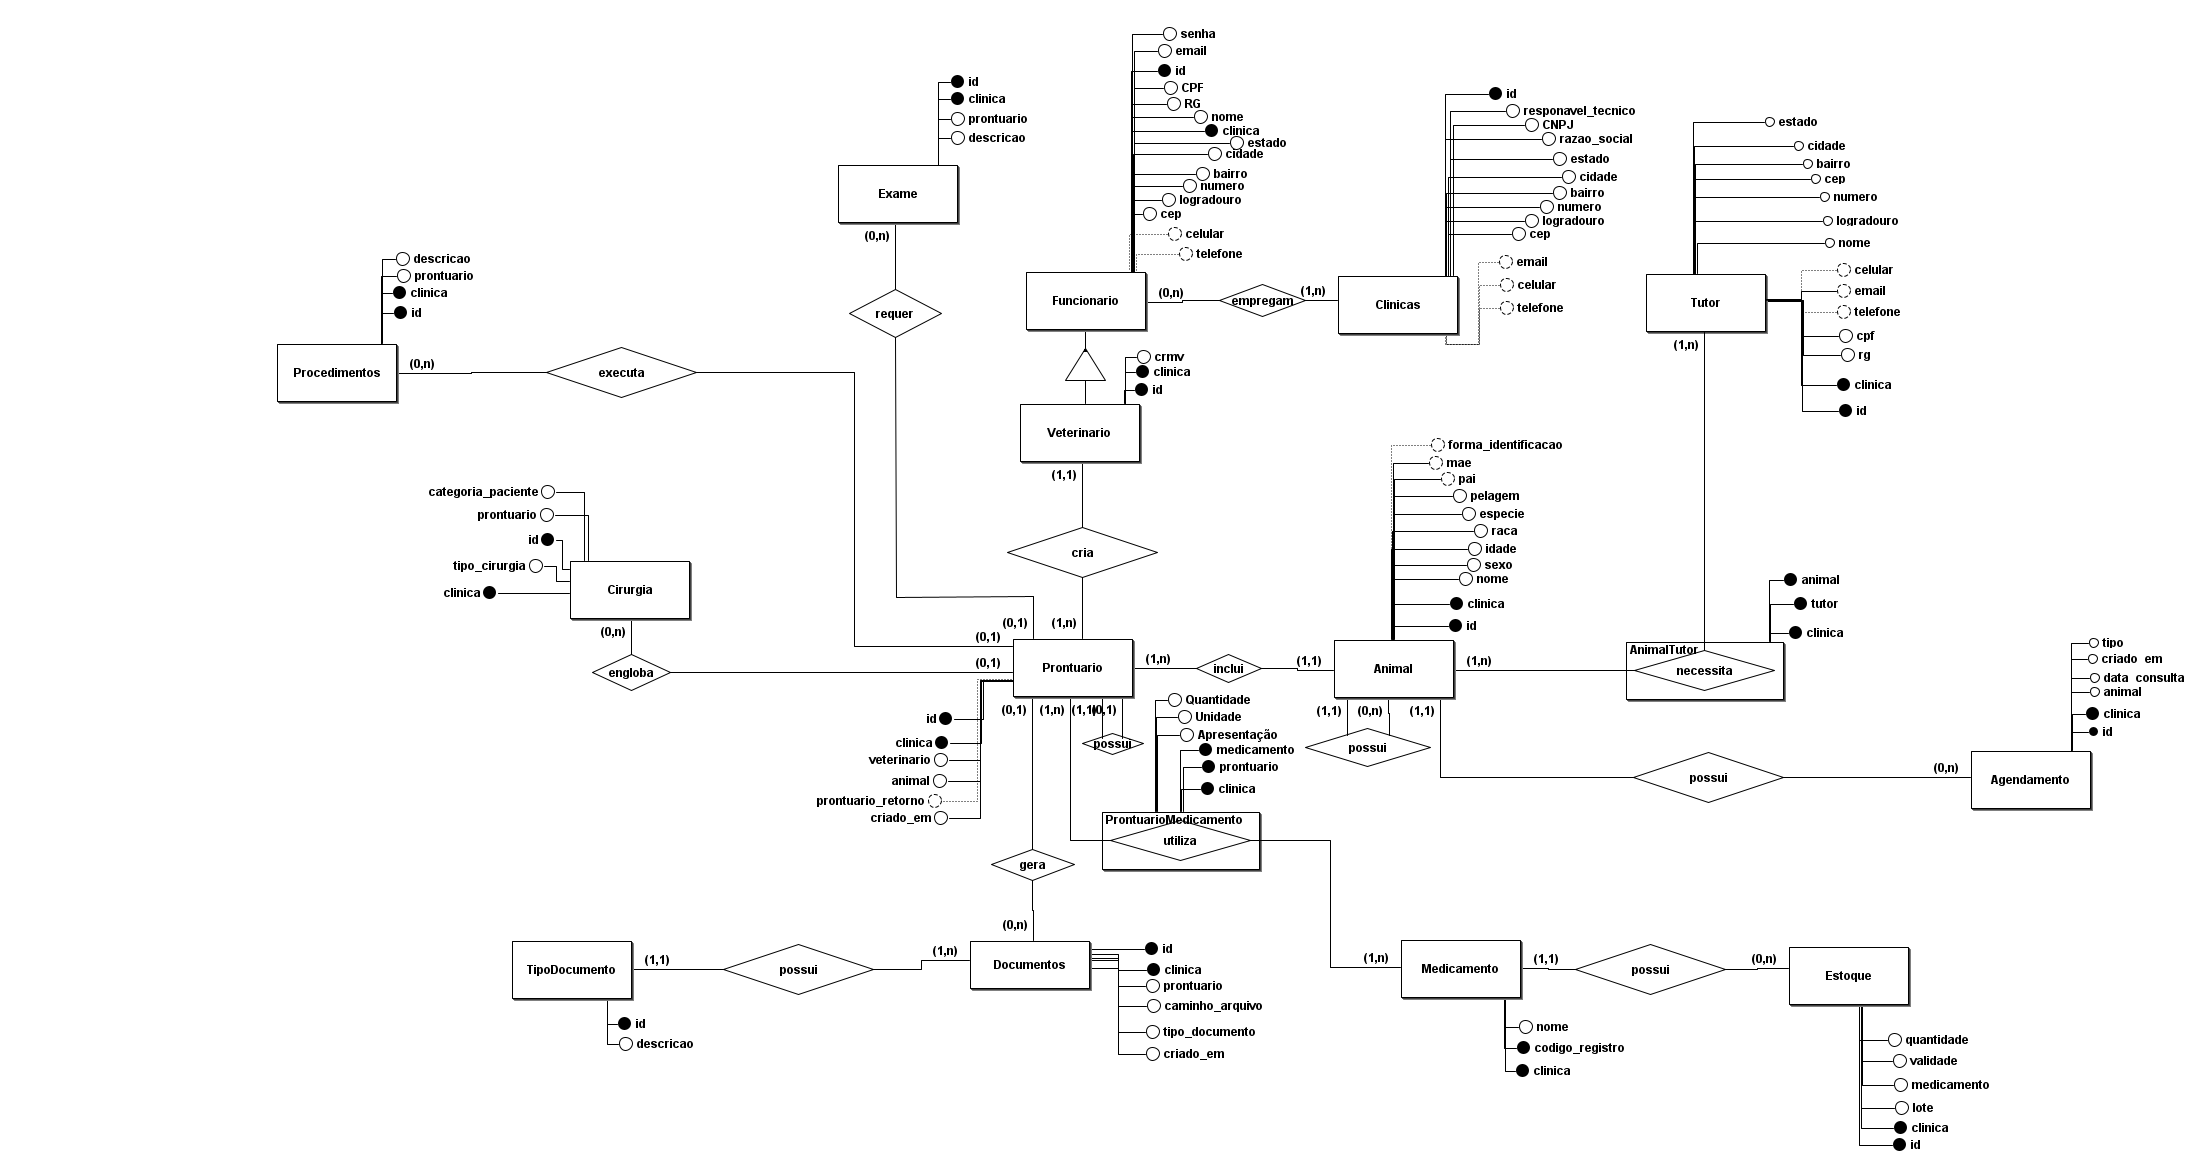
\includegraphics[ width=\linewidth]{images/ProjetoPI1.png}
                \caption{\DIFaddFL{Modelo Entidade Relacionamento}}
                \label{fig:MER}
            \end{figure}

            \begin{center}
                \begin{table}[H]
                \centering
                \caption{\DIFaddFL{Entidades do }\nameref{fig:MER} }
                \begin{tabulary}{1.0\textwidth}{|p{10em}|p{26em}|}
                \hline
                \DIFaddFL{Entidade }& \DIFaddFL{Descrição}\\
                \hline
                \DIFaddFL{Prontuário }& \DIFaddFL{Entidade em que é armazenado os dados do atendimento de um animal. }\\
                \hline
                \DIFaddFL{Veterinário }& \DIFaddFL{Entidade em que é armazenado os dados do profissional veterinário}\DIFaddendFL .\DIFdelbeginFL \DIFdelFL{Esse }\DIFdelendFL \DIFaddbeginFL \\
                \hline
                \DIFaddFL{Animal }& \DIFaddFL{Entidade em que }\DIFaddendFL é \DIFdelbeginFL \DIFdelFL{um processo evolutivo, onde a equipe gradativamente deve se reunir com }\DIFdelendFL \DIFaddbeginFL \DIFaddFL{armazenado os dados do animal.}\\
                \hline
                \DIFaddFL{Medicamento }& \DIFaddFL{Entidade em que é armazenado os dados do medicamento.}\\
                \hline
                \DIFaddFL{ProntuárioMedicamento }& \DIFaddFL{Entidade em que é associado o medicamente com a quantidade utilizada no atendimento.}\\
                \hline
                \DIFaddFL{Estoque }& \DIFaddFL{Entidade que armazena a quantidade disponível do medicamento.}\\
                \hline
                \DIFaddFL{Clínica }& \DIFaddFL{Entidade que armazena dados referentes ao estabelecimento veterinário.}\\
                \hline
                \DIFaddFL{Tutor }& \DIFaddFL{Entidade que armazena dados do tutor/proprietário do animal atendido.}\\
                \hline
                \DIFaddFL{AnimalTutor }& \DIFaddFL{Entidade que associa um animal com seu tutor.}\\
                \hline
                \DIFaddFL{Agendamento }& \DIFaddFL{Entidade que registra um animal com horario de atendimento, clínica e tipo de atendimento.}\\
                \hline
                \DIFaddFL{Funcionário }& \DIFaddFL{Entidade que armazena os dados dos funcionários do estabelecimento.}\\
                \hline
                \DIFaddFL{Documento }& \DIFaddFL{Entidade que armazena dados comuns referentes a documentos obrigatórios gerados pelo veterinário.}\\
                \hline
                \DIFaddFL{TipoDocumento }& \DIFaddFL{Entidade que armazena dados específicos de um documento obrigatório.}\\
                \hline
                \DIFaddFL{Procedimento }& \DIFaddFL{Entidade que armazena dados dos procedimentos realizados.}\\
                \hline
                \DIFaddFL{Cirurgia }& \DIFaddFL{Entidade que armazena dados do tipo de cirurgia realizada.}\\
                \hline
                \DIFaddFL{Exame }& \DIFaddFL{Entidade que armazena dados dos exames solicitados e resultados.}\\
                \hline
                \end{tabulary}

                \label{tab: entidades}
                \end{table}
            \end{center}

            \begin{center}
              \begin{quadro}[H]
              \centering
                  \caption{\DIFadd{Dicionário de Dados - Prontuário}}
                  \begin{tabulary}{1.0\textwidth}{|p{9em}|c|c|c|p{19em}|}
                \hline
                \DIFadd{Atributos }& \DIFadd{Chave }& \DIFadd{NN }& \DIFadd{Tipo }& \DIFadd{Descrição}\\
                \hline
                \DIFadd{Clínica }& \DIFadd{FK }& \DIFadd{x }& \DIFadd{bigint }& \DIFadd{Identifica a qual clínica }\DIFaddend o \DIFdelbegin \DIFdel{Product Owner a fim de refinar os requisitos levantados}\DIFdelend \DIFaddbegin \DIFadd{prontuário pertence }\\
                \hline
                \DIFadd{Veterinário }& \DIFadd{FK }& \DIFadd{x }& \DIFadd{bigint }& \DIFadd{Identifica o veterinário responsável }\\
                \hline
                \DIFadd{Animal }& \DIFadd{FK }& \DIFadd{x }& \DIFadd{bigint }& \DIFadd{Identifica o animal atendido }\\
                \hline
                \DIFadd{Criado Em }& & \DIFadd{x }& \DIFadd{timestamp }& \DIFadd{registro de quando o prontuário foi feito }\\
                \hline
                \DIFadd{Prontuário }& \DIFadd{PK }& \DIFadd{x }& \DIFadd{bigint }& \DIFadd{Identificação do prontuário }\\
                \hline
                \end{tabulary}

                  \label{qd: md-prontuario}
              \end{quadro}
            \end{center}

            \begin{center}
              \begin{quadro}[H]
              \centering
                  \caption{\DIFadd{Dicionário de Dados - Veterinário}}
                  \begin{tabulary}{1.0\textwidth}{|p{9em}|c|c|c|p{19em}|}
                \hline
                \DIFadd{Atributos }& \DIFadd{Chave }& \DIFadd{NN }& \DIFadd{Tipo }& \DIFadd{Descrição}\\
                \hline
                \DIFadd{ID }& \DIFadd{PK }& \DIFadd{x }& \DIFadd{BIGINT }& \DIFadd{Atributo de Identificação do médico veterinário }\\
                \hline
                \DIFadd{CRMV }& \DIFadd{- }& \DIFadd{x }& \DIFadd{varchar }& \DIFadd{Atributo que guarda o registro do médico veterinário}\\
                \hline
                \DIFadd{Clínica }& \DIFadd{FK }& \DIFadd{x }& \DIFadd{BIGINT }& \DIFadd{Atributo que identifica a clínica onde o médico veterinário trabalha}\\
                \hline
                \end{tabulary}

                  \label{qd: md-veterinario}
              \end{quadro}
            \end{center}

            \begin{center}
              \begin{quadro}[H]
              \centering
                  \caption{\DIFadd{Dicionário de Dados - Animal}}
                  \begin{tabulary}{1.0\textwidth}{|p{9em}|c|c|c|p{19em}|}
                \hline
                \DIFadd{Atributos }& \DIFadd{Chave }& \DIFadd{NN }& \DIFadd{Tipo }& \DIFadd{Descrição}\\
                \hline
                \DIFadd{ID }& \DIFadd{PK }& \DIFadd{x }& \DIFadd{BIGINT }& \DIFadd{Identifica a chave do }\\
                \hline
                \DIFadd{Nome }& \DIFadd{- }& \DIFadd{x }& \DIFadd{varchar }& \DIFadd{Atributo que guarda o nome do animal}\\
                \hline
                \DIFadd{Espécie }& \DIFadd{- }& \DIFadd{x }& \DIFadd{varchar }& \DIFadd{Atributo que recebe a especie do animal}\\
                \hline
                \DIFadd{Raça }& \DIFadd{- }& \DIFadd{x }& \DIFadd{varchar }& \DIFadd{Atributo que recebe a raça do animal }\\
                \hline
                \DIFadd{Sexo }& \DIFadd{- }& \DIFadd{x }& \DIFadd{varchar }& \DIFadd{Atributo que recebe o sexo do animal}\\
                \hline
                \DIFadd{Idade }& \DIFadd{- }& \DIFadd{x }& \DIFadd{BIGINT }& \DIFadd{Atributo que recebe a idade do animal}\\
                \hline
                \DIFadd{Pelagem }& \DIFadd{- }& \DIFadd{- }& \DIFadd{varchar }& \DIFadd{Atributo que recebe o tipo de pelagem do animal }\\
                \hline
                \DIFadd{Clínica }& \DIFadd{FK }& \DIFadd{x }& \DIFadd{BIGINT }& \DIFadd{Atributo que identifica a clínica }\\
                \hline
                \DIFadd{Forma\_identificação }& \DIFadd{- }& \DIFadd{- }& \DIFadd{varchar }& \DIFadd{Atributo que recebe a identificação do animal}\\
                \hline
                \DIFadd{Mãe }& \DIFadd{FK }& \DIFadd{- }& \DIFadd{BIGINT }& \DIFadd{Atributo que identifica a mãe do animal }\\
                \hline
                \DIFadd{Pai }& \DIFadd{FK }& \DIFadd{- }& \DIFadd{BIGINT }& \DIFadd{Atributo que identifica o pai do animal }\\
                \hline
                \end{tabulary}

                  \label{qd: md-animal}
              \end{quadro}
            \end{center}

    \begin{center}
      \begin{quadro}[H]
      \centering
          \caption{\DIFadd{Dicionário de Dados - Medicamento}}
          \begin{tabulary}{1.0\textwidth}{|p{9em}|c|c|c|p{19em}|}
        \hline
        \DIFadd{Atributos }& \DIFadd{Chave }& \DIFadd{NN }& \DIFadd{Tipo }& \DIFadd{Descrição}\\
        \hline
        \DIFadd{Id }& \DIFadd{PK }& \DIFadd{x }& \DIFadd{BIGINT }& \DIFadd{Atributo que identifica o medicamento}\\
        \hline
        \DIFadd{Código\_Registro }& \DIFadd{- }& \DIFadd{x }& \DIFadd{BIGINT }& \DIFadd{Atributo que identifica o código do medicamento}\\
        \hline
        \DIFadd{Nome }& \DIFadd{- }& \DIFadd{x }& \DIFadd{varchar }& \DIFadd{Atributo que identifica o nome do medicamento}\\
        \hline
        \DIFadd{Clínica }& \DIFadd{FK }& \DIFadd{x }& \DIFadd{BIGINT }& \DIFadd{Atributo que identifica a clínica que estoca o medicamento}\\
        \hline
        \end{tabulary}

          \label{qd: md-medicamento}
      \end{quadro}
    \end{center}

    \begin{center}
      \begin{quadro}[H]
      \centering
          \caption{\DIFadd{Dicionário de Dados - ProntuárioMedicamento}}
          \begin{tabulary}{1.0\textwidth}{|p{9em}|c|c|c|p{19em}|}
        \hline
        \DIFadd{Atributos }& \DIFadd{Chave }& \DIFadd{NN }& \DIFadd{Tipo }& \DIFadd{Descrição}\\
        \hline
        \DIFadd{Prontuário }& \DIFadd{FK }& \DIFadd{x }& \DIFadd{BIGINT }& \DIFadd{Identificação do Prontuário }\\
        \hline
        \DIFadd{Medicamento }& \DIFadd{FK }& \DIFadd{x }& \DIFadd{BIGINT }& \DIFadd{Atributo que identifica o medicamento utilizado }\\
        \hline
        \DIFadd{Clínica }& \DIFadd{FK }& \DIFadd{x }& \DIFadd{BIGINT }& \DIFadd{Atributo que identifica a clinica do prontuário}\\
        \hline
        \DIFadd{Apresentação }& \DIFadd{- }& \DIFadd{x }& \DIFadd{varchar }& \DIFadd{Atributo que recebe o tipo de apresentação do medicamento}\\
        \hline
        \DIFadd{Quantidade }& \DIFadd{- }& \DIFadd{x }& \DIFadd{BIGINT }& \DIFadd{Atributo que recebe a quantidade do medicamento utilizada}\\
        \hline
        \DIFadd{Unidade }& \DIFadd{- }& \DIFadd{x }& \DIFadd{varchar }& \DIFadd{Atributo que recebe a unidade do medicamento }\\
        \hline
        \end{tabulary}

          \label{qd: md-prontuariomedicamento}
      \end{quadro}
    \end{center}

    \begin{center}
      \begin{quadro}[H]
      \centering
          \caption{\DIFadd{Dicionário de Dados - Estoque}}
          \begin{tabulary}{1.0\textwidth}{|p{9em}|c|c|c|p{19em}|}
        \hline
        \DIFadd{Atributos }& \DIFadd{Chave }& \DIFadd{NN }& \DIFadd{Tipo }& \DIFadd{Descrição}\\
        \hline
        \DIFadd{Id }& & & & \\
        \hline
        \DIFadd{Clínica }& \DIFadd{FK }& \DIFadd{x }& \DIFadd{BIGINT }& \DIFadd{Identifica qual Clínica o Estoque pertence}\\
        \hline
        \DIFadd{Medicamento }& \DIFadd{FK }& \DIFadd{x }& \DIFadd{BIGINT }& \DIFadd{Atributo que identifica o medicamento}\\
        \hline
        \DIFadd{Lote }& \DIFadd{- }& \DIFadd{x }& \DIFadd{BIGINT }& \DIFadd{Atributo que recebe o lote do medicamento}\\
        \hline
        \DIFadd{Validade }& \DIFadd{- }& \DIFadd{x }& \DIFadd{timestamp }& \DIFadd{Atributo que recebe a data de validade do medicamento }\\
        \hline
        \DIFadd{Entrada\_Quantidade }& \DIFadd{- }& \DIFadd{x }& \DIFadd{BIGINT }& \DIFadd{Atributo que recebe a quantidade do medicamento que entra no estoque}\\
        \hline
        \DIFadd{Quantidade }& \DIFadd{- }& \DIFadd{x }& \DIFadd{BIGINT }& \DIFadd{Atributo que recebe a quantidade de medicamento total do estoque }\\
        \hline
        \end{tabulary}

          \label{qd: md-estoque}
      \end{quadro}
    \end{center}

    \begin{center}
      \begin{quadro}[H]
      \centering
          \caption{\DIFadd{Dicionário de Dados - Clínica}}
          \begin{tabulary}{1.0\textwidth}{|p{9em}|c|c|c|p{19em}|}
        \hline
        \DIFadd{Atributos }& \DIFadd{Chave }& \DIFadd{NN }& \DIFadd{Tipo }& \DIFadd{Descrição}\\
        \hline
        \DIFadd{ID }& \DIFadd{PK }& \DIFadd{x }& \DIFadd{BIGINT }& \DIFadd{Atributo que identifica a clínica }\\
        \hline
        \DIFadd{Razao Social }& \DIFadd{- }& \DIFadd{x }& \DIFadd{varchar }& \DIFadd{Atributo que guarda o nome da clínica}\\
        \hline
        \DIFadd{CNPJ }& \DIFadd{- }& \DIFadd{x }& \DIFadd{BIGINT }& \DIFadd{Atributo que guarda o CNPJ da clínica }\\
        \hline
        \DIFadd{Responsável Técnico }& \DIFadd{- }& \DIFadd{x }& \DIFadd{varchar }& \DIFadd{Atributo que recebe o nome do responsável técnico da clínica}\\
        \hline
        \DIFadd{Telefone }& \DIFadd{- }& \DIFadd{x }& \DIFadd{varchar }& \DIFadd{Atributo que recebe o telefone da clínica}\\
        \hline
        \DIFadd{Email }& \DIFadd{- }& \DIFadd{x }& \DIFadd{varchar }& \DIFadd{Atributo que recebe o email da clínica}\\
        \hline
        \DIFadd{Celular }& \DIFadd{- }& \DIFadd{x }& \DIFadd{varchar }& \DIFadd{Atributo que recebe o celular da clínica }\\
        \hline
        \DIFadd{Estado }& \DIFadd{- }& \DIFadd{x }& \DIFadd{varchar }& \DIFadd{Atributo que recebe o estado da clínica}\\
        \hline
        \DIFadd{Cidade }& \DIFadd{- }& \DIFadd{x }& \DIFadd{varchar }& \DIFadd{Atributo que recebe a cidade da clínica }\\
        \hline
        \DIFadd{Bairro }& \DIFadd{- }& \DIFadd{x }& \DIFadd{varchar }& \DIFadd{Atributo que recebe o bairro da clínica }\\
        \hline
        \DIFadd{Logradouro }& \DIFadd{- }& \DIFadd{x }& \DIFadd{varchar }& \DIFadd{Atributo que recebe o nome da rua da clínica}\\
        \hline
        \DIFadd{Número }& \DIFadd{- }& \DIFadd{x }& \DIFadd{varchar }& \DIFadd{Atributo que recebe o número da clínica }\\
        \hline
        \DIFadd{CEP }& \DIFadd{- }& \DIFadd{x }& \DIFadd{varchar }&  \DIFadd{Atributo que recebe o CEP da clinica}\\
        \hline
        \end{tabulary}

          \label{qd: md-clinica}
      \end{quadro}
    \end{center}

    \begin{center}
      \begin{quadro}[H]
      \centering
          \caption{\DIFadd{Dicionário de Dados - Tutor}}
          \begin{tabulary}{1.0\textwidth}{|p{9em}|c|c|c|p{19em}|}
        \hline
        \DIFadd{Atributos }& \DIFadd{Chave }& \DIFadd{NN }& \DIFadd{Tipo }& \DIFadd{Descrição}\\
        \hline
        \DIFadd{ID }& \DIFadd{PK }& \DIFadd{x }& \DIFadd{BIGINT }& \DIFadd{Atributo que identifica o tutor }\\
        \hline
        \DIFadd{Nome }& \DIFadd{- }& \DIFadd{x }& \DIFadd{varchar }& \DIFadd{Atributo que guarda o nome do tutor}\\
        \hline
        \DIFadd{Clínica }& \DIFadd{FK }& \DIFadd{x }& \DIFadd{BIGINT }& \DIFadd{Identifica qual Clínica está registrado}\\
        \hline
        \DIFadd{Rg }& \DIFadd{- }& \DIFadd{x }& \DIFadd{varchar }& \DIFadd{Atributo que recebe o rg do tutor }\\
        \hline
        \DIFadd{CPF }& \DIFadd{- }& \DIFadd{x }& \DIFadd{varchar }& \DIFadd{Atributo que recebe o CPF do tutor}\\
        \hline
        \DIFadd{Email }& \DIFadd{- }& \DIFadd{x }& \DIFadd{varchar }& \DIFadd{Atributo que recebe o email do tutor}\\
        \hline
        \DIFadd{Telefone }& \DIFadd{- }& \DIFadd{x }& \DIFadd{varchar }& \DIFadd{Atributo que recebe o telefone do tutor}\\
        \hline
        \DIFadd{Celular }& \DIFadd{- }& \DIFadd{x }& \DIFadd{varchar }& \DIFadd{Atributo que recebe o celular do tutor}\\
        \hline
        \DIFadd{Estado }& \DIFadd{- }& \DIFadd{x }& \DIFadd{varchar }& \DIFadd{Atributo que recebe o estado do tutor}\\
        \hline
        \DIFadd{Cidade }& \DIFadd{- }& \DIFadd{x }& \DIFadd{varchar }& \DIFadd{Atributo que recebe a cidade do tutor}\\
        \hline
        \DIFadd{Bairro }& \DIFadd{- }& \DIFadd{x }& \DIFadd{varchar }& \DIFadd{Atributo que recebe o bairro do tutor}\\
        \hline
        \DIFadd{Logradouro }& \DIFadd{- }& \DIFadd{x }& \DIFadd{varchar }& \DIFadd{Atributo que recebe o nome da rua do tutor}\\
        \hline
        \DIFadd{Numero }& \DIFadd{- }& \DIFadd{x }& \DIFadd{varchar }& \DIFadd{Atributo que recebe o numero de residencia do tutor}\\
        \hline
        \DIFadd{CEP }& \DIFadd{- }& \DIFadd{x }& \DIFadd{varchar }& \DIFadd{Atributo que recebe o CEP do tutor}\\
        \hline
        \end{tabulary}

          \label{qd: md-tutor}
      \end{quadro}
    \end{center}

    \begin{center}
      \begin{quadro}[H]
      \centering
          \caption{\DIFadd{Dicionário de Dados - AnimalTutor}}
          \begin{tabulary}{1.0\textwidth}{|p{9em}|c|c|c|p{19em}|}
        \hline
        \DIFadd{Atributos }& \DIFadd{Chave }& \DIFadd{NN }& \DIFadd{Tipo }& \DIFadd{Descrição}\\
        \hline
        \DIFadd{Tutor }& \DIFadd{FK }& \DIFadd{x }& \DIFadd{BIGINT }& \DIFadd{Atributo que identifica o tutor. }\\
        \hline
        \DIFadd{Animal }& \DIFadd{FK }& \DIFadd{x }& \DIFadd{BIGINT }& \DIFadd{Atributo que identifica o animal.}\\
        \hline
        \DIFadd{Clínica }& \DIFadd{FK }& \DIFadd{x }& \DIFadd{BIGINT }& \DIFadd{Identifica qual Clínica está registrado.}\\
        \hline
        \end{tabulary}

          \label{qd: md-animaltutor}
      \end{quadro}
    \end{center}

    \begin{center}
      \begin{quadro}[H]
      \centering
          \caption{\DIFadd{Dicionário de Dados - Agendamento}}
          \begin{tabulary}{1.0\textwidth}{|p{9em}|c|c|c|p{19em}|}
        \hline
        \DIFadd{Atributos }& \DIFadd{Chave }& \DIFadd{NN }& \DIFadd{Tipo }& \DIFadd{Descrição}\\
        \hline
        \DIFadd{ID }& \DIFadd{PK }& \DIFadd{x }& \DIFadd{BIGINT }& \DIFadd{Atributo que identifica o agendamento }\\
        \hline
        \DIFadd{Animal }& \DIFadd{FK }& \DIFadd{x }& \DIFadd{BIGINT }& \DIFadd{Atributo que identifica o animal que passará por atendimento }\\
        \hline
        \DIFadd{Clínica }& \DIFadd{FK }& \DIFadd{x }& \DIFadd{BIGINT }& \DIFadd{Identifica qual Clínica o Agendamento foi marcado}\\
        \hline
        \DIFadd{Tipo }& \DIFadd{- }& \DIFadd{x }& \DIFadd{varchar }& \DIFadd{Atributo que recebe o tipo de atendimento será realizado }\\
        \hline
        \DIFadd{Criado\_Em }& \DIFadd{- }& \DIFadd{x }& \DIFadd{timestamp }& \DIFadd{Atributo que guarda a data quando foi realizado o agendamento}\\
        \hline
        \DIFadd{Data\_Consulta }& \DIFadd{- }& \DIFadd{x }& \DIFadd{timestamp }& \DIFadd{Atributo que guarda a data a ser realizado o atendimento }\\
        \hline
        \end{tabulary}

          \label{qd: md-agendamento}
      \end{quadro}
    \end{center}

    \begin{center}
      \begin{quadro}[H]
      \centering
          \caption{\DIFadd{Dicionário de Dados - Funcionário}}
          \begin{tabulary}{1.0\textwidth}{|p{9em}|c|c|c|p{19em}|}
        \hline
        \DIFadd{Atributos }& \DIFadd{Chave }& \DIFadd{NN }& \DIFadd{Tipo }& \DIFadd{Descrição}\\
        \hline
        \DIFadd{ID }& \DIFadd{PK }& \DIFadd{x }& \DIFadd{BIGINT }& \DIFadd{Atributo que identifica o funcionário no sistema }\\
        \hline
        \DIFadd{Nome }& \DIFadd{- }& \DIFadd{x }& \DIFadd{varchar }& \DIFadd{Atributo que recebe o nome do funcionário }\\
        \hline
        \DIFadd{Clínica }& \DIFadd{FK }& \DIFadd{x }& \DIFadd{BIGINT }& \DIFadd{Identifica qual Clínica o Funcionário trabalha}\\
        \hline
        \DIFadd{RG }& \DIFadd{- }& \DIFadd{x }& \DIFadd{varchar }& \DIFadd{Atributo que recebe o RG do funcionário}\\
        \hline
        \DIFadd{CPF }& \DIFadd{- }& \DIFadd{x }& \DIFadd{varchar }& \DIFadd{Atributo que recebe o CPF do funcionário}\\
        \hline
        \DIFadd{Senha }& \DIFadd{- }& \DIFadd{x }& \DIFadd{varchar }& \DIFadd{Atributo da senha de acesso do funcionário ao sistema}\\
        \hline
        \DIFadd{Telefone }& \DIFadd{- }& \DIFadd{- }& \DIFadd{varchar }& \DIFadd{Atributo que recebe o contato telefônico do funcionário}\\
        \hline
        \DIFadd{Celular }& \DIFadd{- }& \DIFadd{x }& \DIFadd{varchar }& \DIFadd{Atributo que recebe o contato móvel do funcionário }\\
        \hline
        \DIFadd{Email }& \DIFadd{- }& \DIFadd{x }& \DIFadd{varchar }& \DIFadd{Atributo que recebe o endereço eletrônico do funcionário}\\
        \hline
        \DIFadd{Estado }& \DIFadd{- }& \DIFadd{- }& \DIFadd{varchar }& \DIFadd{Atributo que recebe o estado da residência do funcionário}\\
        \hline
        \DIFadd{Cidade }& \DIFadd{- }& \DIFadd{- }& \DIFadd{varchar }& \DIFadd{Atributo que recebe a cidade da residência do funcionário}\\
        \hline
        \DIFadd{Bairro }& \DIFadd{- }& \DIFadd{- }& \DIFadd{varchar }& \DIFadd{Atributo que recebe o bairro da residência do funcionário}\\
        \hline
        \DIFadd{Logradouro }& \DIFadd{- }& \DIFadd{- }& \DIFadd{varchar }& \DIFadd{Atributo que recebe a rua da residência do funcinário }\\
        \hline
        \DIFadd{Número }& \DIFadd{- }& \DIFadd{- }& \DIFadd{int }& \DIFadd{Atributo que recebe a numeração da residencia do funcionário}\\
        \hline
        \DIFadd{CEP }& \DIFadd{- }& \DIFadd{- }& \DIFadd{varchar }& \DIFadd{Atributo que recebe o CEP do funcionário}\\
        \hline
        \end{tabulary}

          \label{qd: md-funcionario}
      \end{quadro}
    \end{center}

    \begin{center}
      \begin{quadro}[H]
      \centering
          \caption{\DIFadd{Dicionário de Dados - Documento}}
          \begin{tabulary}{1.0\textwidth}{|p{9em}|c|c|c|p{19em}|}
        \hline
        \DIFadd{Atributos }& \DIFadd{Chave }& \DIFadd{NN }& \DIFadd{Tipo }& \DIFadd{Descrição}\\
        \hline
        \DIFadd{ID }& \DIFadd{PK }& \DIFadd{x }& \DIFadd{BIGINT }& \DIFadd{Atributo que identifica o documento }\\
        \hline
        \DIFadd{Clínica }& \DIFadd{FK }& \DIFadd{x }& \DIFadd{BIGINT }& \DIFadd{Identifica qual Clínica o Documento pertence}\\
        \hline
        \DIFadd{Prontuário }& \DIFadd{FK }& \DIFadd{x }& \DIFadd{BIGINT }& \DIFadd{Identificação do Prontuário }\\
        \hline
        \DIFadd{Tipo\_Documento }& \DIFadd{FK }& \DIFadd{x }& \DIFadd{BIGINT }& \DIFadd{Atributo que identifica tipo  de autorização }\\
        \hline
        \DIFadd{Caminho\_Arquivo }& \DIFadd{- }& \DIFadd{x }& \DIFadd{varchar }& \DIFadd{identifica a url do arquivo na AWS}\\
        \hline
        \DIFadd{Criado\_Em }& \DIFadd{- }& \DIFadd{x }& \DIFadd{timestamp }& \DIFadd{Atributo que identifica a data de criação do documento}\\
        \hline
        \end{tabulary}

          \label{qd: md-documento}
      \end{quadro}
    \end{center}

    \begin{center}
      \begin{quadro}[H]
      \centering
          \caption{\DIFadd{Dicionário de Dados - TipoDocumento}}
          \begin{tabulary}{1.0\textwidth}{|p{9em}|c|c|c|p{19em}|}
        \hline
        \DIFadd{Atributos }& \DIFadd{Chave }& \DIFadd{NN }& \DIFadd{Tipo }& \DIFadd{Descrição}\\
        \hline
        \DIFadd{ID }& \DIFadd{PK }& \DIFadd{x }& \DIFadd{BIGINT }& \DIFadd{Atributo que identifica o documento}\\
        \hline
        \DIFadd{Descrição }& \DIFadd{- }& \DIFadd{- }& \DIFadd{varchar }& \DIFadd{Descreve qual tipo de documento}\\
        \hline
        \end{tabulary}

          \label{qd: md-tipodocumento}
      \end{quadro}
    \end{center}

    \begin{center}
      \begin{quadro}[H]
      \centering
          \caption{\DIFadd{Dicionário de Dados - Procedimento}}
          \begin{tabulary}{1.0\textwidth}{|p{9em}|c|c|c|p{19em}|}
        \hline
        \DIFadd{Atributos }& \DIFadd{Chave }& \DIFadd{NN }& \DIFadd{Tipo }& \DIFadd{Descrição}\\
        \hline
        \DIFadd{ID }& \DIFadd{PK }& \DIFadd{x }&\DIFadd{BIGINT }& \DIFadd{Atributo de identificação do exame}\\
        \hline
        \DIFadd{Prontuário }& \DIFadd{FK }& \DIFadd{x }& \DIFadd{BIGINT }& \DIFadd{Identificação do Prontuário }\\
        \hline
        \DIFadd{Clínica }& \DIFadd{FK }& \DIFadd{x }& \DIFadd{BIGINT }& \DIFadd{Identifica em qual Clínica o Procedimento foi realizado}\\
        \hline
        \DIFadd{Descrição }& \DIFadd{- }& \DIFadd{- }& \DIFadd{varchar }& \DIFadd{Descreve o procedimento realizado }\\
        \hline
        \end{tabulary}

          \label{qd: md-Procedimento}
      \end{quadro}
    \end{center}

   \begin{center}
      \begin{quadro}[H]
      \centering
          \caption{\DIFadd{Dicionário de Dados - Cirurgia}}
          \begin{tabulary}{1.0\textwidth}{|p{9em}|c|c|c|p{19em}|}
        \hline
        \DIFadd{Atributos }& \DIFadd{Chave }& \DIFadd{NN }& \DIFadd{Tipo }& \DIFadd{Descrição}\\
        \hline
        \DIFadd{ID }& \DIFadd{PK }& \DIFadd{x }& \DIFadd{BIGINT }& \DIFadd{Atributo de identificação da cirurgia}\\
        \hline
        \DIFadd{Prontuário }& \DIFadd{FK }& \DIFadd{x }& \DIFadd{BIGINT }& \DIFadd{Identificação do Prontuário }\\
        \hline
        \DIFadd{Clínica }& \DIFadd{FK }& \DIFadd{x }& \DIFadd{BIGINT }& \DIFadd{Identifica em qual Clínica a Cirurgia foi realizada}\\
        \hline
        \DIFadd{Categoria\_Paciente }& \DIFadd{- }& \DIFadd{x }& \DIFadd{varchar }& \DIFadd{Identifica a categoria ASA do paciente }\\
        \hline
        \DIFadd{Tipo\_Cirurgia }& \DIFadd{- }& \DIFadd{x }& \DIFadd{varchar }& \DIFadd{Descrição da cirurgia a ser realizada }\\
        \hline
        \end{tabulary}

          \label{qd: md-Cirurgia}
      \end{quadro}
    \end{center}
    \begin{center}
      \begin{quadro}[H]
      \centering
          \caption{\DIFadd{Dicionário de Dados - Exame}}
          \begin{tabulary}{1.0\textwidth}{|p{9em}|c|c|c|p{19em}|}
        \hline
        \DIFadd{Atributos }& \DIFadd{Chave }& \DIFadd{NN }& \DIFadd{Tipo }& \DIFadd{Descrição}\\
        \hline
        \DIFadd{ID }& \DIFadd{PK }& \DIFadd{x }& \DIFadd{BIGINT }& \DIFadd{Atributo de identificação do Exame}\\
        \hline
        \DIFadd{Clínica }& \DIFadd{FK }& \DIFadd{x }& \DIFadd{BIGINT }& \DIFadd{Identifica a qual Clínica o Exame pertence}\\
        \hline
        \DIFadd{Prontuário }& \DIFadd{FK }& \DIFadd{x }& \DIFadd{BIGINT }& \DIFadd{Identificação do Prontuário }\\
        \hline
        \DIFadd{Descrição }& \DIFadd{- }& \DIFadd{- }& \DIFadd{varchar }& \DIFadd{Nome do Exame }\\
        \hline
        \end{tabulary}

          \label{qd: md-Exame}
      \end{quadro}
    \end{center}

        \subsection{\DIFadd{Modelo lógico}}

            \begin{figure}[H]
                \centering
                \includegraphics[width=0.7\textwidth]{images/Modelo Lógico.png}
                \caption{\DIFaddFL{Modelo Lógico}}
                \label{fig:DER}
            \end{figure}

    \section{\DIFadd{Gestão e organização da equipe}}

        \subsection{\DIFadd{Organização da Equipe}}

            \DIFadd{O guia do scrum declara explícitamente que o time deve ser pequeno suficiente para que seja ágil e grande o suficiente para que possa desempenhar trabalho relevante, recomendando o envolvimento de não mais que 10 integrantes.\mbox{%DIFAUXCMD
\cite{scrum2}
            }\hskip0pt%DIFAUXCMD
}

            \DIFadd{Orientados pela recomendação de formação de papéis da equipe ágil scrum, foram definidos 3 papéis para ser desempenhado pelos membros da equipe: Product Owner (PO -  Dono do Produto), Scrum Master (SCM - Mestre do Scrum) e Developers, que foram denominados Team Members (TM - Membros da equipe). Esses papéis têm o objetivo de apontar facilitadores e atribuir responsabilidades em pontos específicos do projeto, não havendo um responsável isolado ou encarregado do bom desenvolvimento das atividades.\mbox{%DIFAUXCMD
\cite{scrum2} }\hskip0pt%DIFAUXCMD
\mbox{%DIFAUXCMD
\cite{agile2}
            }\hskip0pt%DIFAUXCMD
}

            \DIFadd{O PO é responsável por definir clara e objetivamente como as funcionalidades da aplicação devem se comportar, compreender e priorizar a necessidade de negócio que melhor atende a necessidade do usuário (stakeholders) e que o back log seja visível e disponível para todos os membros do time.\mbox{%DIFAUXCMD
\cite{agile2} }\hskip0pt%DIFAUXCMD
O papel será desempenhado pela Irina Chang.
            }

            \DIFadd{O SCM tem a responsabilidade que o time consiga desenvolver autonomia, destravando entendimentos e facilitando a identificação de dinâmicas que resultem em melhor entregabilidade das atividades.\mbox{%DIFAUXCMD
\cite{agile2} }\hskip0pt%DIFAUXCMD
O papel será desempenhado por Henrique.
            }

            \DIFadd{Team Member é a forma como foi decidido denominar o papel dos desenvolvedores. Estes serão os responsáveis pela implementação de código}\DIFaddend , \DIFdelbegin \DIFdel{resultando }\DIFdelend \DIFaddbegin \DIFadd{padronização de commits, integrações, modelagem de banco de dados, além de verificar se as alterações propostas pelo PO são tecnicamente viáveis de serem implementadas, definindo os processos necessários para a implementação. Por consequência, são os maiores responsáveis pelo desenvolvimento da documentação do código e garantia da manutenibilidade. Independentemente do envolvimento anterior, são responsáveis por auxiliar em  manutenções futuras e realizar a entrega (deploy) da aplicação }\DIFaddend em \DIFdelbegin \DIFdel{itens do Product Backlog. Partindo das regras de negócio, }\DIFdelend \DIFaddbegin \DIFadd{produção.\mbox{%DIFAUXCMD
\cite{scrum2} }\hskip0pt%DIFAUXCMD
Os team members }\DIFaddend são\DIFdelbegin \DIFdel{apresentados os requisitos funcionais, }\DIFdelend \DIFaddbegin \DIFadd{: Caique Daniel, Luis Renato, Marcos Querino, Murilo Pires e Welen Mota.
            }

            \DIFadd{Entretanto, diferentemente do papel do scrum, o time conta com indivíduos com conhecimentos e habilidades diversas e tempo limitado para o desenvolvimento do projeto. Dessa forma, os papeis servirão como referência, mas }\DIFaddend não \DIFdelbegin \DIFdel{funcionais e por fim as histórias }\DIFdelend \DIFaddbegin \DIFadd{limitam os indivíduos às atividades definidas pelos papéis do scrum. A tabela abaixo foi elaborada para facilitar a identificação da ênfase }\DIFaddend de \DIFdelbegin \DIFdel{usuário}\DIFdelend \DIFaddbegin \DIFadd{atuação de cada indivíduo sobre as atividades desempenhadas.
            }

            %DIF >  Fonte: https://scrumguides.org/scrum-guide.html#scrum-team
            %DIF >  Fonte https://www.atlassian.com/br/agile/scrum/roles
            %DIF >  Revisão fim %

   \begin{center}
        \begin{table}[h]
        \centering
        \resizebox{16cm}{!}{%
            \begin{tabular}{|p {15}|rrrrrrrr|}
            \hline
            \multicolumn{1}{|c|}{Membro}      & \multicolumn{1}{c|}{Irina}   & \multicolumn{1}{r|}{Henrique} & \multicolumn{1}{r|}{Caique}       & \multicolumn{1}{r|}{Luís} &
            \multicolumn{1}{r|}{\begin{tabular}[c]{@{}c@{}}Marcos \end{tabular}}  &
            \multicolumn{1}{r|}{Murilo} & \multicolumn{1}{r|}{Welen}\\ \hline

    \multicolumn{1}{|l|}{\begin{tabular}[c]{@{}c@{}}Documentação \end{tabular}} &
         \multicolumn{1}{c|}{x}  & \multicolumn{1}{c|}{x}  & \multicolumn{1}{c|}{x}  & \multicolumn{1}{c|}{x}  & \multicolumn{1}{c|}{x}  & \multicolumn{1}{c|}{x}  & \multicolumn{1}{c|}{x}            \\ \hline
    \multicolumn{1}{|l|}{\begin{tabular}[c]{@{}c@{}}Front-end \end{tabular}}&                 
        \multicolumn{1}{c|}{ }  & \multicolumn{1}{c|}{ }  & \multicolumn{1}{c|}{ x }  & \multicolumn{1}{c|}{x}  & \multicolumn{1}{c|}{x}    & \multicolumn{1}{c|}{ }  & \multicolumn{1}{c|}{ }            \\ \hline

    \multicolumn{1}{|l|}{\begin{tabular}[c]{@{}c@{}}Back-end \end{tabular}} &
        \multicolumn{1}{c|}{x} & \multicolumn{1}{c|}{x}  & \multicolumn{1}{c|}{} & \multicolumn{1}{c|}{}  & \multicolumn{1}{c|}{} & \multicolumn{1}{c|}{x}  & \multicolumn{1}{c|}{}            \\ \hline

  \multicolumn{1}{|l|}{\begin{tabular}[c]{@{}c@{}}Banco de dados \end{tabular}} &
        \multicolumn{1}{c|}{}  & \multicolumn{1}{c|}{}  & \multicolumn{1}{c|}{x} & \multicolumn{1}{c|}{}  & \multicolumn{1}{c|}{}  & \multicolumn{1}{c|}{}  & \multicolumn{1}{c|}{}            \\ \hline

    \multicolumn{1}{|l|}{\begin{tabular}[c]{@{}c@{}}Infraestrutura \end{tabular}} &
        \multicolumn{1}{c|}{ }  & \multicolumn{1}{c|}{x} & \multicolumn{1}{c|}{ } & \multicolumn{1}{c|}{ } & \multicolumn{1}{c|}{ } & \multicolumn{1}{c|}{ }  & \multicolumn{1}{c|}{ }            \\ \hline

   \end{tabular}%
       }
        \caption{\DIFaddFL{Membros}}
        \label{tab:membros}
        \end{table}
    \end{center}

    
     

    \subsection{\DIFadd{Gestão de projeto}}

        %DIF >  Revisão inicio %
        %DIF > Estou com duvidas com relação a esse primeiro paragrafo
        \DIFadd{A partir da avaliação dos requisitos, considerou-se que não existem funcionalidades com processos claramente definidos até o início do desenvolvimento de cada processo e o tempo hábil para elaborar e documentar extensamente todos os processos para serem implementados não é suficiente para que exista código a ser implementado. Portanto, a abordagem de planejamento de projetos cascata não é adequada para desenvolver a solução}\DIFaddend .

        \DIFdelbegin \subsection{\DIFdel{Regras de Negócio}}
%DIFAUXCMD
\addtocounter{subsection}{-1}%DIFAUXCMD
\DIFdel{As regras de negócio são as premissas necessárias para a modelagem do projeto e }\DIFdelend \DIFaddbegin \DIFadd{Em contrapartida, devido a característica mutável dos requisitos e restrição temporal definida pelo cronograma acadêmico, ocorreu o entendimento que adaptar elementos das metodologias Scrum \mbox{%DIFAUXCMD
\cite{scrum} }\hskip0pt%DIFAUXCMD
e XP \mbox{%DIFAUXCMD
\cite{agile} }\hskip0pt%DIFAUXCMD
seriam melhor adequados às necessidades do projeto. Enfatizando o emprego dos processos, rituais e cerimônias do Scrum e complementando com elementos do método XP para o dia a dia de desenvolvimento, favoreceu que os membros tenham maior propensão à colaboração e dinamismo de desenvolvimento, resultando em entregas com ritmo constante e incremental.
        }

        \DIFadd{Os ciclos para o desenvolvimento do projeto foram projetados com duração semanal, denominadas Sprint. Este processo é definido no Scrum como o período em que ocorrem os desenvolvimentos, sendo um dos conceitos centrais da metodologia. Define o escopo que será trabalhado, movendo os itens que passam do backlog para a etapa de refinamento e desenvolvimento pela equipe, analisa e desenvolve os elementos que comporão a solução, podendo negociar novos prazos com o PO conforme a equipe identifica novos aprendizados\mbox{%DIFAUXCMD
\cite{scrum}}\hskip0pt%DIFAUXCMD
. Este processo permite melhor acompanhamento da evolução do desenvolvimento, permitindo manter os stakeholders atualizados e com expectativas alinhadas.
        }

        \DIFadd{Ao final de cada Sprint, ocorre a cerimônia de Sprint Review para discutir o processo de aprendizado do período, quais os resultados obtidos e avaliar a evolução da semana, }\DIFaddend através \DIFdelbegin \DIFdel{delas serão definidas as regras básicas as quais o sistema deve concernir.
        Tem por objetivo explicitar as restrições a serem adotadas pelo sistema a fim de não fugir do escopo delimitado para completa resolução do problema}\DIFdelend \DIFaddbegin \DIFadd{de debate sobre dificuldades, soluções e impedimentos encontrados no decorrer da Sprint. Também é realizado o planejamento da Sprint da semana seguinte, analisando e priorizando os próximos itens que passarão do backlog para serem trabalhados no próximo ciclo de desenvolvimento durante as Sprint Plannings, conforme a recomendações de \mbox{%DIFAUXCMD
\citeonline{scrum} }\hskip0pt%DIFAUXCMD
para o Scrum.
        }

        \DIFadd{Como abordagem para o dia a dia provinda do método XP, a prática de pair programing é adotada para estimular o desenvolvimento colaborativo no time. Essa abordagem permite maior compartilhamento dos conhecimentos de cada indivíduo}\DIFaddend , de forma \DIFdelbegin \DIFdel{a definir como melhor compreender as disponibilidades das funcionalidades, tal qual a interdependência entre as mesmas. O Quadro X dispõe das informações referente às regras de negócios do Sidekick}\DIFdelend \DIFaddbegin \DIFadd{mais coesa e analisada por pares durante o desenvolvimento do código ou documento. Tal abordagem reduz possíveis atrasos no desenvolvimento decorrentes de dúvidas ou entraves individuais, tendo como consequência a entrega de código com consistência e validação por pares. A abordagem também aumenta o envolvimento do time em relação a entrega de código com qualidade, derivado do sentimento de responsabilidade coletiva que nasce da autonomia para modificações\mbox{%DIFAUXCMD
\cite{agile}}\hskip0pt%DIFAUXCMD
}\DIFaddend .

        \DIFdelbegin \subsection{\DIFdel{Requisitos Funcionais}}
%DIFAUXCMD
\addtocounter{subsection}{-1}%DIFAUXCMD
\DIFdel{No Quadro Y são apresentados os requisitos funcionais, onde tem-se a materialização das necessidades e especificações das ações que o sistema deve executar, ignorando as limitações físicas, focando apenas no comportamento de entrada e saída do sistema}\DIFdelend \DIFaddbegin \DIFadd{A abordagem aprofunda o conhecimento específico da equipe sobre determinado assunto e da solução construída e incentiva o compartilhamento e comunicação entre os integrantes envolvidos imediatamente durante o desenvolvimento ou durante a Sprint Review.
        }

        \DIFadd{Abaixo estão relacionados as tabelas de desenvolvimento do projeto referentes as Sprints semanais, a divisão de tarefas Epics e o Product Backlog do desenvolvimento do projeto.
        %DIF >  Revisão fim %
        }\begin{center}
      \begin{quadro}[H]
      \centering
          \caption{\DIFadd{Cronograma das Sprints}}
          \begin{tabulary}{1.0\textwidth}{|p{8em}|p{8em}|p{19em}|}
        \hline
        \DIFadd{Início }& \DIFadd{Fim }& \DIFadd{Descrição}\\
        \hline
        \DIFadd{09/08/2022/ }& \DIFadd{16/08/2022 }& \DIFadd{Definição de grupo e discussão inicial sobre temas. }\\
        \hline
        \DIFadd{16/08/2022 }& \DIFadd{23/08/2022 }& \DIFadd{Apresentação das propostas aos professores e escolha do projeto.}\\
        \hline
        \DIFadd{23/08/2022 }& \DIFadd{30/08/2022 }& \DIFadd{Apresentação inicial dos projetos, aprovação do tema e divisão das atividades.}\\
        \hline
        \DIFadd{30/08/2022 }& \DIFadd{06/09/2022 }& \DIFadd{Início da modelagem da aplicação}\DIFaddend .\DIFaddbegin \\
        \hline
        \DIFadd{06/09/2022 }& \DIFadd{13/09/2022 }& \DIFadd{Início do desenvolvimento da modelagem de dados.}\\
        \hline
        \DIFadd{13/09/2022 }& \DIFadd{20/09/2022 }& \DIFadd{Escolha da arquitetura da aplicação.}\\
        \hline
        \DIFadd{20/09/2022 }& \DIFadd{27/09/2022 }& \DIFadd{Discussão de Regras de negócio, Requisitos e Custo do Projeto. }\\
        \hline
        \DIFadd{27/09/2022 }& \DIFadd{04/10/2022 }& \DIFadd{Apresentação do Desenho da aplicação e definição dos próximos passos. }\\
        \hline
        \DIFadd{04/10/2022 }& \DIFadd{11/10/2022 }& \DIFadd{Semana de desenvolvimento e preparação para a apresentação da POC. }\\
        \hline
        \DIFadd{11/10/2022 }& \DIFadd{18/10/2022 }& \DIFadd{Ajustes finais para a apresentação da POC. }\\
        \hline
        \DIFadd{18/10/2022 }& \DIFadd{25/10/2022 }& \DIFadd{Hands on de implementações e ajustes de documentação.}\\
        \hline
        \DIFadd{25/10/2022 }& \DIFadd{01/11/2022 }& \DIFadd{Discussão e desenvolvimento da documentação e evolução do MVP da aplicação. }\\
        \hline
        \DIFadd{01/11/2022 }& \DIFadd{08/11/2022 }& \DIFadd{Desenvolvimento final da documentação e da aplicação do MVP.}\\
        \hline
        \end{tabulary}
         \DIFaddend 

          \DIFdelbegin \subsection{\DIFdel{Requisitos não Funcionais}}
%DIFAUXCMD
\addtocounter{subsection}{-1}%DIFAUXCMD
\DIFdel{Os requisitos não funcionaistratam-se de restrições mais técnicas do projeto}\DIFdelend \DIFaddbegin \label{qd: sprints}
      \end{quadro}
    \end{center}

    %DIF >   Criação do BACKLOG  %

 \begin{center}
      \begin{quadro}[H]
      \centering
          \caption{\DIFadd{Epics}}
          \begin{tabulary}{1.0\textwidth}{|p{12em}|p{25em}|}
        \hline
       \DIFadd{Epic }& \DIFadd{Descrições  }\\
        \hline
        \DIFadd{Ajustes Documentação }& \DIFadd{Mudanças ao longo do projeto na documentação (documentação como um todo)}\\
        \hline
        \DIFadd{Ajustes Administrativos }& \DIFadd{Atualizações Gource, SVN, Métricas, posts no blog}\\
        \hline
        \DIFadd{Desenvolvimento POC }& \DIFadd{Front-end: funcionalidades front-end desenvolvidas na POC.
        Back-end: funcionalidades back-end desenvolvidas na POC}\\
        \hline
        \DIFadd{Desenvolvimento MVP }& \DIFadd{Front-end: funcionalidades front end desenvolvidas no MVP.
      Back-end: funcionalidades back end desenvolvidas no MVP}\\
        \hline
        \end{tabulary}
          \label{qd: epic}
      \end{quadro}
    \end{center}

    
    \begin{center}
      \begin{quadro}[H]
      \centering
          \caption{\DIFadd{Product Backlog}}
          \begin{tabulary}{1.0\textwidth}{|p{6em}|p{5em}|p{24em}|}
        \hline
       \DIFadd{Entregar até }& \DIFadd{Prioridade }& \DIFadd{Descrição }\\
        \hline
         \DIFadd{30/08/2022 }& \DIFadd{Alta }& \DIFadd{Definir tema final que será desenvolvido no projeto, realizar apresentação do tema definido}\\
         \hline
         \DIFadd{13/09/2022 }& \DIFadd{Alta }& \DIFadd{Realizar a modelagem do MER e DER para suportar a aplicação, validar com os clientes}\\
         \hline
         \DIFadd{20/09/2022 }& \DIFadd{Alta }& \DIFadd{Realizar o desenho de arquitetura do sistema}\DIFaddend , \DIFdelbegin \DIFdel{são as necessidades que não }\DIFdelend \DIFaddbegin \DIFadd{validar com os integrantes do time as tecnologias utilizadas, validar com os clientes.}\\
        \hline
         \DIFadd{27/09/2022 }& \DIFadd{Alta }& \DIFadd{Definir regras de negócios do sistema, definir requisitos funcionais, casos de uso, histórias de usuários, custos do projeto}\\
         \hline
         \DIFadd{27/09/2022 }& \DIFadd{Alta }& \DIFadd{Configurar ambiente RDS; Configurar Docker; Configurar aplicações em springboot; Configurar aplicações em React}\\
        \hline
        \DIFadd{11/10/2022 }& \DIFadd{Alta }& \DIFadd{Desenvolver funcionalidades de autenticar usuário e registrar usuário no banco de dados na AWS. }\\
        \hline
        \DIFadd{11/10/2022 }& \DIFadd{Media }& \DIFadd{Entregar funcionalidades registro CRMV, entendimento da viabilidade da funcionalidades, alinhar por e-mail com a CFMV.}\\
        \hline
         \DIFadd{18/10/2022 }& \DIFadd{Alta }& \DIFadd{Entregar funcionalidades levantadas no escopo da POC, apresentar para os clientes as funcionalidades.}\\
        \hline
         \DIFadd{25/10/2022 }& \DIFadd{Alta }& \DIFadd{Realizar ajustes e correções da POC, Realizar melhorias na proposta da aplicação, realizar ajustes na documentação com o feedback dos clientes }\\
        \hline
        \DIFadd{01/11/2022 }& \DIFadd{Alta }& \DIFadd{Realizar desenvolvimento funcionalidades x (MVP)
        desenvolvimento funcionalidades y (MVP)
        Ajustes finais na documentação}\\
        \hline
         \DIFadd{08/11/2022 }& \DIFadd{Alta }& \DIFadd{Entrega da documentação do projeto, feedbacks do cliente e definições para a apresentação do MVP}\\
        \hline
        \DIFadd{22/11/2022 }& \DIFadd{Alta }& \DIFadd{Entrega da apresentação do MVP e feedback dos clientes.}\\
        \hline
        \end{tabulary}

          \label{qd: backlog}
      \end{quadro}
    \end{center}

    %DIF >  % % %

    \subsection{\DIFadd{Ferramenta de gestão}}

        \DIFadd{Após definir as funcionalidades que serão desenvolvidas, foi constatada a necessidade de geri-las a partir de uma ferramenta de gestão de projetos.
        }

        \DIFadd{Sistemas como Microsoft Project e similares }\DIFaddend são \DIFdelbegin \DIFdel{atendidas necessariamente através de funcionalidades}\DIFdelend \DIFaddbegin \DIFadd{ideais para projetos que empregam a abordagem do modelo cascata. Como não proveem a flexibilidade para mudanças e velocidade de aprendizado que projetos ágeis exigem, foi optado pelo uso da ferramenta Jira Software, disponível no modelo gratuito e on cloud.
        }

        \DIFadd{Como ferramenta de mercado, o Jira Software é uma ferramenta de gestão de projetos flexível, reconhecida por dar suporte a diferentes abordagens de gestão de projeto, mas amplamente utilizado em projetos que envolvem metodologias ágeis\mbox{%DIFAUXCMD
\cite{jira}}\hskip0pt%DIFAUXCMD
.
        }

        \DIFadd{No contexto do desenvolvimento da aplicação, as atividades serão divididas em Épicos, que conterão Histórias e Tarefas, que serão distribuídas por quadros Kanban. Estes quadros permitem maior flexibilidade nos processos de gestão das atividades, organizando o fluxo de trabalho com as tarefas planejadas, em progresso e entregues\mbox{%DIFAUXCMD
\cite{jira}}\hskip0pt%DIFAUXCMD
.
        }

        %DIF >  Revisão fim %

    \section{\DIFadd{Arquitetura}}

        %DIF >  Revisão inicio %

        %DIF > O sistema foi desenvolvido com base no modelo de arquitetura cliente-servidor, abordando a divisão de camadas e a separação no que consiste em back-end e front-end da aplicação. Por meio de um navegador web, os clientes fazem as requisições ao servidor, que é acessível através de uma API (Application Programming Interface) REST responsável por lidar com as regras de negócio e com a comunicação entre as camadas. O Elastic Load Balancing tem como responsabilidade distribuir esse tráfego de entrada entre as duas instâncias EC2, uma contendo o back end e outra o front end, ambas em ambientes isolados pelo Docker Container, onde o back end possui integrado a ele o CloudWatch Logs para monitoramento dos logs da aplicação. Toda essa parte de serviços operacionais do sistema está inclusa no AWS Elastic BeanStalk, provedor de máquina e serviços necessários de forma a abstrair detalhes de infraestrutura para a implementação da aplicação.

        %DIF > Como banco de dados relacional da aplicação, foi empregado o serviço gerenciado de banco de dados AWS RDS para MySQL. Este serviço permite o funcionamento do banco de forma abstraída, enquanto, para o armazenamento de arquivos estáticos da aplicação, como os documentos pdf emitidos pela aplicacão CertVet, foi empregado o serviço Amazon S3.

        

        %DIF >  Antes %
        %DIF >  ------------- %
        %DIF >  Depois %

        \DIFadd{A aplicação está hospedada na infra estrutura da provedora de nuvem pública AWS. A provedora fornece todos os recursos computacionais e serviços necessários para que a solução seja executada, além de prover VPC (Virtual Private Cloud), que atua como rede interna e Security Groups, que atua como firewall.
        }

        \DIFadd{O sistema foi desenvolvido com base no modelo de arquitetura cliente-servidor, empregando a abordagem de divisão em camadas back-end e front-end para maior desacoplamento.
        }

        \DIFadd{O cliente, ao fazer uma requisição via navegador web ao nosso endereço web, recebe a aplicação de front-end que está hospedada no container da aplicação React da respectiva instância EC2, que permitirá que seja processada pelo próprio navegador.
        }

        \DIFadd{Por meio da interface web, as diversas intâncias dos clientes fazem requisições ao servidor, utilizando o padrão REST APIs(Reprentational State Application Programming Interface).
        Assim, o servidor presente na instância EC2 que roda o container da aplicação Java Spring boot fica responsável por resolver as regras de negócio e comunicar seus resultados entre as demais camadas.
        }

        \DIFadd{Como parte da integração com terceiros, a aplicação de back-end prevê realizar requisições ao servidor externo de domínio da entidade de classe CRMV.
           }

        \DIFadd{O serviço Elastic Load Balancing tem como responsabilidade distribuir o tráfego de dentro e fora da VPC entre as possíveis instâncias EC2 que processam as requisições da aplicação e seus clientes, em caso de escalonamento vertical ou horizontal da aplicação.
        }

        \DIFadd{Para que seja possível armazenar os logs da aplicação, o back-end está integrado ao serviço CloudWatch Logs. Este serviço permite que os logs da aplicação possam ser monitorados de fora do servidor de instalação da aplicação.
        }

        \DIFadd{O serviço operacional é provisionado pelo AWS Elastic BeanStalk, que abstrai o processo de requisição e reserva de recursos de infraestrutura que implementa da aplicação.
        }

        \DIFadd{O banco de dados relacional responsável pelo armazenamento dos dados da aplicação é o MySQL provido pelo AWS RDS, serviço gerenciado que persiste os estados gerados pela lógica de negócio de forma abstraída, enquanto, para o armazenamento de arquivos estáticos da aplicação, como os documentos gerados pela aplicação CertVet, fora utilizado o armazenamento de objetos Amazon S3 como banco de dados não relacional.
        }

        \DIFadd{Para armazenamento das imagens da solução}\DIFaddend , \DIFdelbegin \DIFdel{objetivando garantir níveis satisfatórios  de desempenho, disponibilidade, escalabilidade, dentre outras garantias que permitam a máxima usabilidade do sistema. Os requisitos }\DIFdelend \DIFaddbegin \DIFadd{está previsto o serviço da provedora docker, mas }\DIFaddend não \DIFdelbegin \DIFdel{funcionais que compreendem ao Sidekick são elencados no Quadro Z, apresentado a seguir}\DIFdelend \DIFaddbegin \DIFadd{é restrito a este provedor.
        }

        \DIFadd{O esquema da arquitetura do sistema pode ser vista mais detalhadamente na figura abaixo.
        }

        %DIF >  Revisão fim %

        \begin{figure}[H]
            \centering
            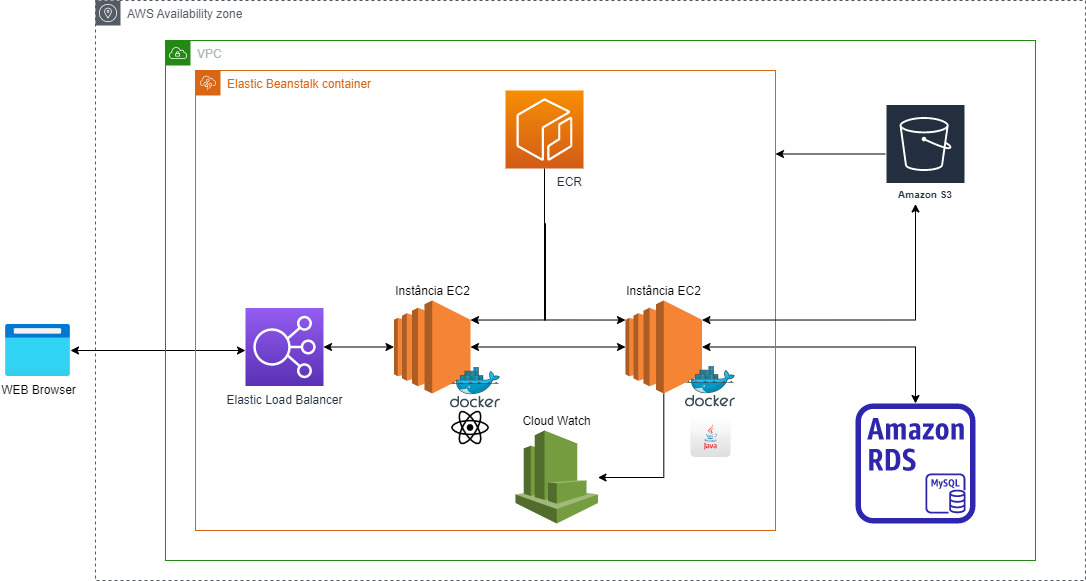
\includegraphics[width=0.9\textwidth]{ArquiteturaAplicacao.png}
            \caption{\DIFaddFL{Infraestrutura}}
            \label{fig:infra}
        \end{figure}

        \subsubsection{\DIFadd{Elastic Load Balancing}}

            \DIFadd{Serviço que distribui o tráfego externo à infra estrutura entre instâncias de processamento da aplicação. Em diversos cenários de aplicações, a tecnologia permite que uma solução seja escalável de forma horizontal para um numero de instâncias de tamanhos variáveis de acordo com a parametrização do gestor da solução}\DIFaddend .

        \DIFdelbegin \section{\DIFdel{Tecnologias e Ferramentas Utilizadas no Projeto}}
%DIFAUXCMD
\addtocounter{section}{-1}%DIFAUXCMD
\DIFdel{O foco atual }\DIFdelend \DIFaddbegin \subsubsection{\DIFadd{Docker Container}}

            \DIFadd{Tecnologia que isola o ambiente da aplicação através }\DIFaddend da \DIFaddbegin \DIFadd{segregação de recursos em namespaces e imagem de }\DIFaddend aplicação\DIFdelbegin \DIFdel{é a plataforma WEB (desktop e navegadores), tendo em vista remover a necessidade de }\DIFdelend \DIFaddbegin \DIFadd{, permitindo maior liberdade no uso dos recursos computacionais de execução em ambiente isolado e portabilidade.
            }

            \DIFadd{Normalmente toma como ponto de partida a distribuição Alpine Linux, que tem o objetivo de ter apenas os recursos necessários para o sistema operacional, aumentando o controle do desenvolvedor sobre os utilitários do sistema operacional.
    }

            \DIFadd{Para a aplicação back end, será empregada uma imagem baseada na pilha amazon linux e amazon correto 17.
            }

        \subsubsection{\DIFadd{AWS Elastic BeanStalk}}

            \DIFadd{Serviço gerenciado que abstrai a necessidade de tomar decisão sobre recursos físicos da aplicação, provisionando máquina e serviços necessários para a implementação da solução. Provê suporte à tecnologia Docker container.
            }

        \subsubsection{\DIFadd{Amazon ECR - Amazon Elastic Container Registry}}

            \DIFadd{Similar ao serviço Docker Hub, é um serviço de armazenamento e registro de imagens de containers gerenciado pelo provedor AWS. Permite que seja possível realizar implantações (deploy) automatizados a partir da atualização da imagem Docker armazenada no diretório em nuvem.
}

        \subsubsection{\DIFadd{AWS RDS (Relational Database Service) - Amazon AWS}}

            \DIFadd{Serviço gerenciado que provê banco de dados com redundância em infraestrutura abstraída, suporta implementações de banco de dados relacionais: Amazon Aurora, MySQL, MariaDB, PostgreSQL, Oracle e Microsoft SQL Server. Disponibiliza as funcionalidades de uso mais recorrentes por aplicações.
            }

            \DIFadd{Para a implementação da solução, identificou-se que o uso de uma instância MySQL se enquadra melhor às necessidades da aplicação por não existir necessidade imediata de atender altos volume de transações com o banco de dados.
            }

        \subsubsection{\DIFadd{Amazon S3}}

            \DIFadd{serviço de armazenamento de objetos (no caso da Certvet, documentos de resultado de exames) que oferece escalabilidade. 
}

    \section{\DIFadd{Tecnologias de Desenvolvimento}}

        \DIFadd{Aproveitando da maturidade de frameworks e bibliotecas front end e a complexicidade adicional do desenvolvimento de aplicações dedicadas para ambientes desktop e móveis, com ênfase me celulares (necessidade de permissão de máquina para }\DIFaddend instalação e configuração da aplicação \DIFdelbegin \DIFdel{no ambiente do cliente e utilizar de ferramentas de alta qualidade muito bem conhecidas no mercado para reduzir o tempo de desenvolvimento. }\DIFdelend \DIFaddbegin \DIFadd{em ambiente heterogêneo além de particularidades pontuais de cada cliente), o foco da aplicação foi voltado para a plataforma WEB (navegadores desktop e móveis).
        }\DIFaddend 

        \DIFdelbegin \DIFdel{A fim de realizar a prototipação, a equipe utilizará a }\DIFdelend \DIFaddbegin \DIFadd{Para prototipação, foi utilizada a }\DIFaddend ferramenta Figma, \DIFaddbegin \DIFadd{um }\DIFaddend editor colaborativo online de design gráfico que permite a criação de interfaces de usuário\DIFdelbegin \DIFdel{e que ajudará os }\DIFdelend \DIFaddbegin \DIFadd{. A ferramenta auxilia }\DIFaddend desenvolvedores a construir telas coesas e baseadas nos conceitos e práticas de User Experience (UX) e User Interface (UI). \DIFdelbegin %DIFDELCMD < 

%DIFDELCMD < %%%
\DIFdel{Para o desenvolvimentodo front-end do sistema, foi definido utilizar o Typescript, uma linguagem de programação fortemente tipada de código aberto desenvolvida pela Microsoft, e o SCSS, uma linguagem de script que é transpilada para CSS. Também }\DIFdelend \DIFaddbegin \DIFadd{Como ferramenta de desenvolvimento, a plataforma GitHub }\DIFaddend será \DIFdelbegin \DIFdel{utilizado o ReactJS, uma biblioteca desenvolvida pelo Facebook para a criação de interfaces WEB baseada na utilização de componentes, e o Bootstrap, um framework front-end que fornece estruturas de CSS para a criação de sites e aplicações responsivas de forma rápida e simples}\DIFdelend \DIFaddbegin \DIFadd{usada como principal ferramenta de versionamento dos  repositórios do projeto}\DIFaddend .

        Com o objetivo de facilitar o processo de implementação de uso da ferramenta nos estabelecimentos dos usuários, a instalação de um software como aplicação desktop poderia influenciar negativamente à adoção da aplicação. Ainda, de acordo com as habilidades técnicas \DIFdelbegin \DIFdel{atuais }\DIFdelend dos membros da equipe, foi optado por utilizar tecnologias web baseadas em servidores de aplicação remotos e gerenciados, oferencendo o Software como serviço (SaaS).

        A oferta de software como serviço permite que atualizações e correções sejam implementadas mais rapidamente \DIFdelbegin \DIFdel{já que }\DIFdelend \DIFaddbegin \DIFadd{por }\DIFaddend não \DIFdelbegin \DIFdel{dependem }\DIFdelend \DIFaddbegin \DIFadd{depender }\DIFaddend da interferência em infraestrutura de responsabilidade do cliente. Adicionalmente, \DIFdelbegin \DIFdel{é mais provável que a }\DIFdelend \DIFaddbegin \DIFadd{reduz-se o risco de }\DIFaddend instalação do serviço \DIFdelbegin \DIFdel{foi realizada adequadamente}\DIFdelend \DIFaddbegin \DIFadd{de forma inadequada}\DIFaddend .

    \subsection{\DIFdelbegin \DIFdel{Front end}\DIFdelend \DIFaddbegin \DIFadd{Front-end}\DIFaddend }

        A pilha de tecnologias de desenvolvimento para o front end se concentram nas ferramentas e tecnologias:

        \begin{itemize}

            \item Figma: Editor colaborativo online de design gráfico que permite a criação de interfaces de usuário e que ajudará os desenvolvedores a construir telas coesas e baseadas nos conceitos e práticas de User Experience (UX) e User Interface (UI).

            \item Typescript:
                Linguagem que permite programação fortemente tipada de código aberto desenvolvida pela Microsoft lançada em 1 de outubro de 2012. 

                É também um supertipo da linguagem  JavaScript, o que significa que possui todas as funcionalidades do JavaScript e além da adição de novos recursos. 

                Essa linguagem foi selecionada para desenvolver o front end devido a complexidade e escala da aplicação, que requer estruturas de dados mais complexas do que o JavaScript pode oferecer suporte, fazendo-se necessário a utilização de uma linguagem com tipagem de dados forte. 

                Outro motivo que colaborou para a escolha foi a segurança, já que graças a tipagem de dados, erros que podem causar vulnerabilidades e passam despercebidos em aplicações desenvolvidas com JavaScript serão identificados no momento da compilação do TypeScript para JavaScript.

            \item SCSS:
                Linguagem de estilização para WEB compilada para CSS.

                Essa linguagem foi selecionada para estilizar o front end da aplicação pelo fato de possuir compatibilidade com o CSS e também uma melhor estrutura organizacional de código quando comparado com o CSS.

            \item ReactJS:
                Biblioteca JavaScript/TypeScript desenvolvida pelo Facebook para a criação de interfaces WEB lançada em 29 de maio de 2013. O React foi escolhido graças a arquitetura baseada em componentes que permite a reutilização dos mesmo em diferentes partes da aplicação. Os componentes são escritos utilizando JSX que possui uma sintaxe semelhante ao HTML, o que o torna fácil de utilizar.

            \item Bootstrap:
                Framework front end que fornece estruturas de CSS para a criação de sites e aplicações responsivas de forma rápida e simples.

                Essa tecnologia foi escolhida pelo fato de reduzir consideravelmente o tempo de desenvolvimento da estilização da interface da aplicação com om usuário.

        \end{itemize}

        \subsection{\DIFdelbegin \DIFdel{Back end}\DIFdelend \DIFaddbegin \DIFadd{Back-end}\DIFaddend }

            Para compor a pilha de tecnologias aplicadas no back end, foi definido utilizar as seguintes tecnologias:

            \begin{itemize}
                \item Java 17: 
                    Linguagem de programação fortemente tipada com ênfase no paradigma de desenvolvimento orientado a objeto. É amplamente empregada em aplicações comerciais e cientificas maduras, tanto open source como privadas.

                    A partir da comunidade de desenvolvimento, projetos open source de permissionamento livre permite acesso a bibliotecas e ferramentas como framework Demoiselle, para assinatura de documentos que cumprem a especificação ICP-Brasil.

                    A versão 17 é uma versão LTS - Long Term Service, permite o emprego das tecnologias e funcionalidades mais recentes da linguagem, sem prejuízo às implementações mais antigas.

                \item Framework Spring Boot: 
                    Framework mais amplamente utilizado da linguagem Java para aplicações de uso geral, permite integração sem quebras entre dependências de bibliotecas e frameworks especializados como Spring MVC, hibernate ou Apache Kafka.
                    \begin{itemize}
                        \item ORM - spring JPA (Hibernate)
                        \item Spring Web - controllers
                        \item Apache Tomcat - Servidor HTTP
                        \item Hibernate Validator
                        \item Mockito - Framework que auxilia o desenvolvimento de testes de unidade
                        \item SL4J - Framework dedicado ao registro de logs
                    \end{itemize}
                \item Banco de dados Mysql:
                    Banco de dados relacional com ampla implementação de provedores de tecnologias em nuvem aberta ou on premisses, tendo licença permissiva de uso e familiaridade aos membros da equipe.
            \end{itemize}

        \DIFdelbegin \subsection{\DIFdel{Infraestrutura}}
    %DIFAUXCMD
\addtocounter{subsection}{-1}%DIFAUXCMD
%DIFDELCMD < 

%DIFDELCMD <         \includegraphics[width=0.9\textwidth]{ArquiteturaAplicacao.drawio.png}
%DIFDELCMD <     

%DIFDELCMD <         %%%
\subsubsection{\DIFdel{Docker Container}}
%DIFAUXCMD
\addtocounter{subsubsection}{-1}%DIFAUXCMD
%DIFDELCMD < 

%DIFDELCMD <             %%%
\DIFdel{Tecnologia que isola o ambiente da aplicação através da segregação de recursos em namespaces e imagem de aplicação, permitindo maior liberdade no uso dos recursos computacionais de execução em ambiente isolado e portabilidade.
            }%DIFDELCMD < 

%DIFDELCMD <             %%%
\DIFdel{Normalmente toma como ponto de partida a distribuição Alpine Linux, que tem o objetivo de ter apenas os recursos necessários para o sistema operacional, aumentando o controle do desenvolvedor sobre os utilitários do sistema operacional.
    }%DIFDELCMD < 

%DIFDELCMD <             %%%
\DIFdel{Para a aplicação back end, será empregada uma imagem baseada na pilha amazon linux e amazon correto 17.
            }%DIFDELCMD < 

%DIFDELCMD <         %%%
\subsubsection{\DIFdel{AWS Elastic BeanStalk}}
%DIFAUXCMD
\addtocounter{subsubsection}{-1}%DIFAUXCMD
%DIFDELCMD < 

%DIFDELCMD <             %%%
\DIFdel{Serviço gerenciado que abstrai a necessidade de tomar decisão sobre recursos físicos da aplicação, provisionando máquina e serviços necessários para a implementação da solução. Provê suporte à tecnologia Docker container.
            }%DIFDELCMD < 

%DIFDELCMD <         %%%
\subsubsection{\DIFdel{Amazon ECR - Amazon Elastic Container Registry}}
        %DIFAUXCMD
\addtocounter{subsubsection}{-1}%DIFAUXCMD
%DIFDELCMD < 

%DIFDELCMD <             %%%
\DIFdel{Similar ao serviço Docker Hub, é um serviço de armazenamento e registro de imagens de containers gerenciado pelo provedor AWS. Permite que seja possível realizar implantações (deploy) automatizados a partir da atualização da imagem Docker armazenada no diretório em nuvem.
}%DIFDELCMD < 

%DIFDELCMD <         %%%
\subsubsection{\DIFdel{AWS RDS (Relational Database Service) - Amazon AWS}}
%DIFAUXCMD
\addtocounter{subsubsection}{-1}%DIFAUXCMD
%DIFDELCMD < 

%DIFDELCMD <             %%%
\DIFdel{Serviço gerenciado que provê banco de dados com redundância em infraestrutura abstraída, suporta implementações de banco de dados relacionais: Amazon Aurora, MySQL, MariaDB, PostgreSQL, Oracle e Microsoft SQL Server. Disponibiliza as funcionalidades de uso mais recorrentes por aplicações.
            }%DIFDELCMD < 

%DIFDELCMD <             %%%
\DIFdel{Para a implementação da solução, identificou-se que o uso de uma instância MySQL se enquadra melhor às necessidades da aplicação por não existir necessidade imediata de atender altos volume de transações com o banco de dados.
    }%DIFDELCMD < 

%DIFDELCMD <     %%%
\subsection{\DIFdel{Diagrama Entidade Relacionamento}}
    %DIFAUXCMD
\addtocounter{subsection}{-1}%DIFAUXCMD
%DIFDELCMD < 

%DIFDELCMD <     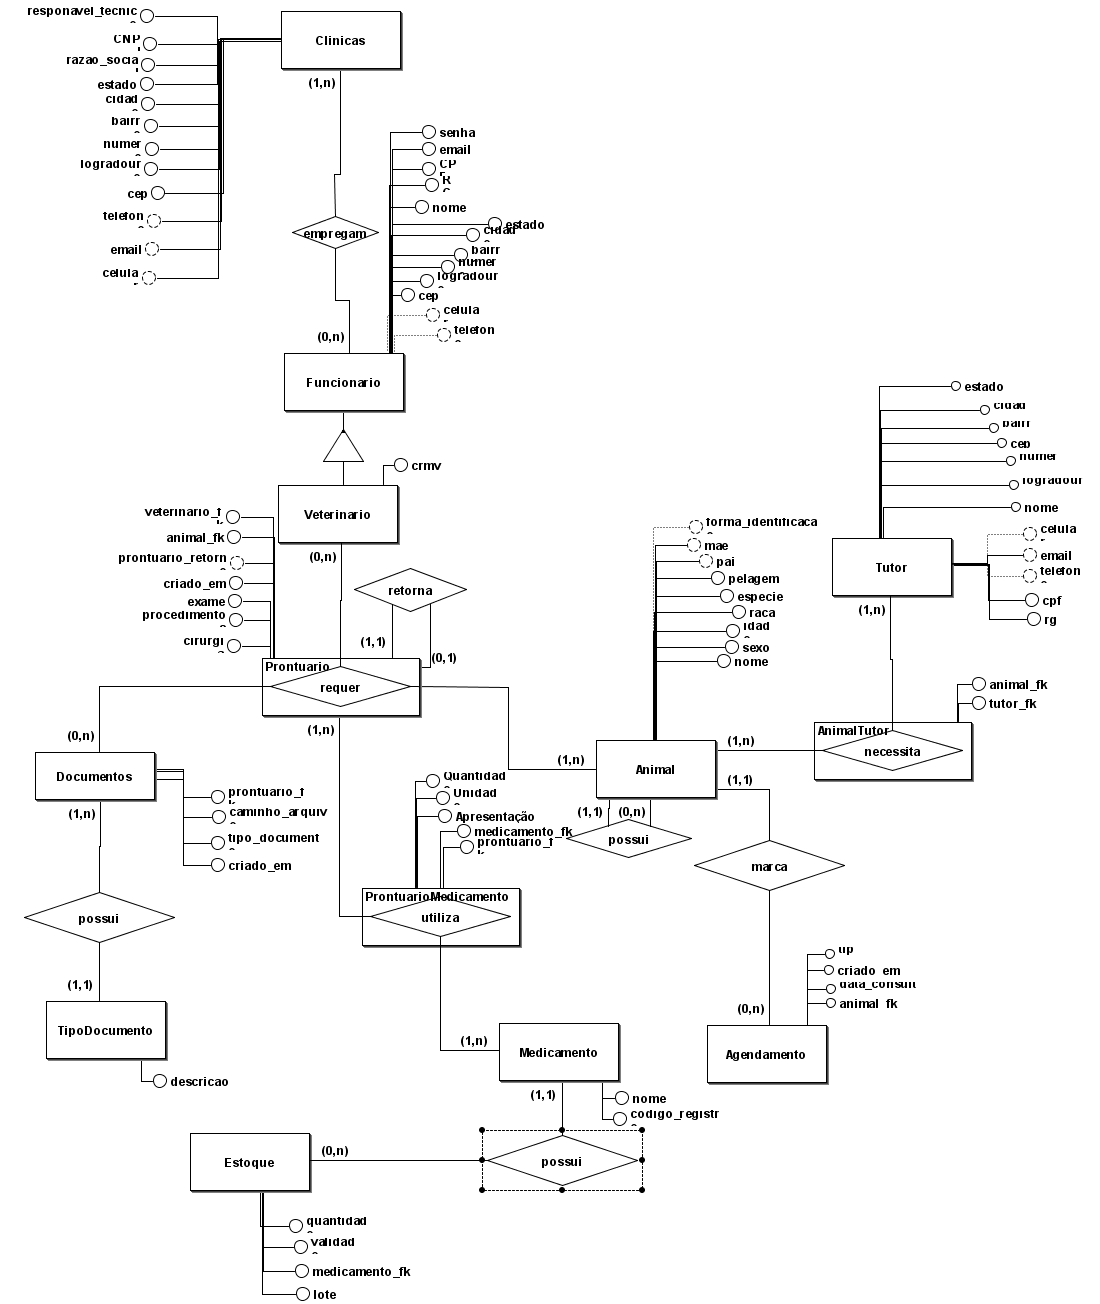
\includegraphics[width=0.9\textwidth]{images/ProjetoPI1.2.png}
%DIFDELCMD <     

%DIFDELCMD <     %%%
\subsection{\DIFdel{Modelo lógico}}
    %DIFAUXCMD
\addtocounter{subsection}{-1}%DIFAUXCMD
%DIFDELCMD < 

%DIFDELCMD <     \includegraphics[width=0.9\textwidth]{images/Modelo_LógicoPI1.2.png}
%DIFDELCMD <     

%DIFDELCMD <     %%%
\DIFdelend \subsection{Ferramentas de testes automatizados}

            Com o objetivo de testar a aplicação e também garantir que as funções retornem os resultados esperados de forma a garantir a integração das partes da mesma, teste unitários são fundamentais para alcançar esses objetivos. Portanto, a equipe utilizará as ferramentas de testes automatizados listados a seguir:

            \begin{itemize}
                \item Jest: é um framework de testes para JavaScript/TypeScript desenvolvido a partir do framework Jasmine, também para testes automatizados.
                \item JUnit: é um framework open-source de teste para a linguagem Java desenvolvido por Erich Gamma e Kent Beck. é assumido por padrão pelo framework Spring e suas ferramentas (Spring Boot).
            \end{itemize}

    

    \DIFaddbegin \section{\DIFadd{Manutenibilidade}}
    \DIFadd{Visando garantir boa resposta dos clientes, atingindo um elevado nível de qualidade, torna-se necessário estabelecer determinados requisitos e parâmetros de manutenibilidade e ferramentas que possam auxiliar esse processo. Partindo desses critérios, é possível mensurar o quanto o desenvolvimento do sistema apresenta conformidade com as boas práticas e, consequentemente, na qualidade do projeto.
}

        \subsection{\DIFadd{Code Convention}}
        \DIFadd{Buscando facilitar o fluxo de trabalho com um maior nível de legibilidade para todos os envolvidos no desenvolvimento do código e, consequentemente, simplificar a integração entre as diferentes partes do que está a ser desenvolvido, a equipe optou por adotar uma convenção de código. Visando o desenvolvimento de um código consistente e transparente, a convenção permite que os diferentes membros possam adicionar contribuições sem grandes dificuldades, aumentando a taxa de transferência e diminuindo o tempo de entrega, resultando em uma base de código mais uniforme e consequentemente impactando na facilidade da manutenção do código.
}

        \subsubsection{\DIFadd{Codificação geral}}
        \DIFadd{A convenção adotada para a parte mais generalizada do código, é a mais comumente usada para o desenvolvimento utilizando a linguagem Java, sendo relativamente próxima dos padrões adotados em outras linguagens populares como JavaScript e Python. As regras seguem como base as sugestões de Coding Convention da Oracle, mas foram adaptadas para as necessidades da equipe:
}

        \begin{itemize}
            \item
            \DIFadd{Declaração de atributos e variáveis em português.
            }\item
            \DIFadd{Nomes de atributos e váriaveis devem ser redigidos em camelCase.
            }\item
            \DIFadd{Variáveis declaradas próximas de onde são inicializadas.
            }\item
            \DIFadd{Declarações globais preferencialmente no início do arquivo.
            }\item
            \DIFadd{Uso reduzido de variáveis, funções e objetos globais.
            }\item
            \DIFadd{Métodos nomeados com camelCase e prefixados com verbo em inglês que deixe claro o que o método faz.
            }\item
            \DIFadd{As constantes devem utilizar notação Upper case, utilizando underscore para separação das palavras em caso de nome composto.
            }\item
            \DIFadd{Nomes de classes e interfaces redigidos em PascalCase.
        }\end{itemize}

    \DIFadd{Somando-se a isso, a resolução do back-end é dividida em pacotes para melhor distribuição e visibilidade da mesma. Sendo eles, o pacote model contendo as classes de modelo, também usadas como entidades mapeadas do banco de dados, o pacote controller contendo o gerenciamento da lógica do negócio através dos controladores e endpoints do serviço, o pacote service contendo a implementação da lógica de negócio através dos serviços e o pacote repository para centralizar as regras de armazenamento dos beans de entidade no sistema.
}

    \subsubsection{\DIFadd{Commits}}
    \DIFadd{A equipe optou por adotar os prefixos gerados pelo Jira, ferramenta utilizada para o gerenciamento de tarefas, para nomear as branchs que serão commitadas tanto no front-end quanto no back-end.
}

    \DIFadd{ERI-X: sendo ERI o prefixo base gerado pelo Jira e X o número de identificação daquela tarefa no dashboard.
}

    \DIFadd{Somado à padronização, fora adotada a prática de efetuar pull requests e o code review por parte de um outro integrante do time, evitando que uma implementação ou alteração seja adicionada diretamente na branch principal do repositório.
}

    \subsection{\DIFadd{Design Patterns e boas práticas}}
    \DIFadd{Visando a padronização do projeto, o time adotou dois padrões comumente usados pela comunidade de desenvolvedores: Builder e Facade, sendo este último adotado pensando na redução do acoplamento entre as diferentes camadas do projeto e na diminuição da complexidade da API e o padrão Builder para isolar a complexidade da criação dos objetos, facilitando a criação das diferentes implementações, todas baseadas em uma mesma interface.
}

    \subsubsection{\DIFadd{Clean Code}}
    \DIFadd{Somado ao Code Convention abordado anteriormente, o Clean Code é um conjunto de práticas de desenvolvimento a fim de garantir que o código seja legível para todos e que, consequentemente, implique em uma manutenção mais ordenada e simplificada, evitando gargalos haja vista que propaga maior inteligibilidade por parte dos desenvolvedores. As práticas adotadas pela equipe podem ser lidas abaixo:
}

    \begin{itemize}
        \item 
        \DIFadd{Definição significativa dos nomes de classes, atributos, métodos, objetos e variáveis.
        }\item
        \DIFadd{Uso de ENUM e constantes para padronização de números que façam sentido no código.
        }\item
        \DIFadd{Criação de funções simples, de procedimentos transparentes e pequenas.
        }\item
        \DIFadd{Uso reduzido de comentários que não sejam necessários.
        }\item
        \DIFadd{Evitar a redundância e a repetição de código.
        }\item
        \DIFadd{Reduzir ao máximo as dependências, de forma a aumentar o desacoplamento e a independência entre as partes do projeto.
        }\item
        \DIFadd{Realizar o tratamento de erros para garantir que o código continuará fazendo o que foi programado para fazer.
        }\item
        \DIFadd{Cobrir e validar todos os processos sensíveis e importantes com testes limpos.
    }\end{itemize}

    \subsubsection{\DIFadd{SOLID}}
    \DIFadd{O conjunto de cinco princípios básicos, denominado na área por SOLID, tem como principal objetivo garantir a maior qualidade no processo de desenvolvimento de software, resultando em uma aplicação mais fácil de ser testada, mantida, corrigida, haja vista a flexibilidade gerada no código em se adequar às possíveis mudanças e até mesmo escalada. No que tange ao entendimento da equipe sobre os princípios e como os mesmos serão aplicados no projeto:
}

    \begin{itemize}
        \item 
        \DIFadd{SRP (Single Responsability Principle), o princípio da responsabilidade única, basicamente determina que uma classe deve ter simplesmente um único motivo para existir, uma única responsabilidade.
        }\item 
        \DIFadd{OCP (Open-closed Principle), ou princípio aberto-fechado, o segundo princípio prevê que uma entidade deve ser aberta para a extensão e fechada para a modificações.
        }\item 
        \DIFadd{LSP (Liskov Substitution Principle), o terceiro
        princípio, o de substituição de Liskov, determina que uma classe que seja derivada deve ser substituível por sua classe originária.
        }\item 
        \DIFadd{ISP (Interface Segregation Principle), o princípio da segregação da interface prevê que uma classe não deve implementar interfaces que possuem atributos e métodos que ela não utilizará.
        }\item 
        \DIFadd{DIP (Dependency Inversion Principle), o quinto princípio, o da inversão de dependência determina que uma classe deve sim depender de abstrações, no entanto, jamais depender de implementações.
    }\end{itemize}

        \subsection{\DIFadd{Logs}}
        \DIFadd{A fim de monitorar o sistema em tempo real de execução, principalmente no que tange à camada do servidor, o time adotou o CloudWatch Logs, ferramenta da Amazon para visualização destes, tornando possível o monitoramento do estado dos objetos. Através de diferentes registros como: info, warn, debug e error, a equipe tem a sua disposição insumos para consultar os dados de log da aplicação, monitorar os logs de instâncias do Amazon EC2 e arquivá-los com segurança para futuras análises, quando necessário, de forma que, quando ocorrer falha do sistema, um log poderá ser consultado para devidas identificações, análises e resoluções.
}

    
    \DIFaddend \section{Segurança}

        \DIFaddbegin \DIFadd{A aplicação, por tratar dados pessoais que podem identificar indivíduo, precisa utilizar métodos seguros e que cumpram regulamentação legal e específica como parte dos requisitos.
    }

        \DIFaddend \subsection{Comunicação}
        \DIFaddbegin 

            \DIFaddend A aplicação utilizará interfaces de aplicação de transferência representacional de estado (REST API), tomando como base o protocolo HTTP.

            O protocolo HTTP (Hyper Text Transfer Protocol) realiza comunicação através de interfaces da arquitetura cliente-servidor. Tanto nos modelos conceituais TCP/IP e OSI (Open System Interconnection) está compreendido pela camada de aplicação. \cite{PetersonRedes}.

            Por permitir comunicação na arquitetura cliente-servidor sem criptografia (trafega dados através de texto simples pelas das camadas de rede), é considerado uma forma não segura de troca de dados.

            Para que a comunicação possa ocorrer sem perda de dados ou interceptação entre as partes, é necessário adicionar criptografia TLS (Transport Layer Security) ou SSL (Secure Socket Layer, base do TLS) na comunicação ponto a ponto, estendendo o protocolo para HTTPS (Hyper Text Transfer Protocol Secure). \cite{PetersonRedes}.

        \subsection{Privacidade}
        \DIFaddbegin 

            \DIFaddend Em diversos sistemas, tanto mobile como web, diversas informações são trocadas entre o usuário e o servidor a todo instante. Dentre essas informações é possível destacar documentos pessoais, senhas e informações sigilosas. Visto isso, uma das prioridades do sistema a ser desenvolvido será a privacidade de seus usuários e de suas informações.

            A lei 13.709/2018, conhecida como LGPD (Lei Geral de Proteção de Dados Pessoais) foi concebida com intuito de disciplinar o uso de dados pessoais por instituições, empoderando a pessoa física sobre os direitos fundamentais da liberdade e privacidade sobre seus dados. \cite{lgpd}

            A lei dispõe sobre atividades em que ocorra "tratamento de dados". Como explica o tribunal de justiça de São Paulo (TJ-SP):

            \begin{quote}
                Considera-se “tratamento de dados” qualquer atividade que utilize um dado pessoal na execução da sua operação, como, por exemplo: coleta, produção, recepção, classificação, utilização, acesso, reprodução, transmissão, distribuição, processamento, arquivamento, armazenamento, eliminação, avaliação ou controle da informação, modificação, comunicação, transferência, difusão ou extração.
            \end{quote}

            Tanto a Serpro quanto o TJ-SP relatam que a lei prevê três agentes das instituições, listando suas respectivas responsabilidades principais:

            \begin{quote}
                Controlador: Responsável pelas decisões relativas ao tratamento dos dados
                Operador: Delegado pelo Controlador, operacionaliza as decisões do Controlador
                Encarregado: Atender às demandas dos titulares, interagir com a autoridade nacional de proteção de dados (ANPD) e orientar funcionários e contratados sobre as práticas de proteção de dados.
            \end{quote}

            O titular dos dados é aquele que pode ter dados que identificam a pessoa natural, sendo tratados , distribuídos ou armazenados. Para que os dados possam ser armazenados nos termos da lei, é necessário que exista expressa autorização pelo titular dos dados, devidamente armazenados para fins de fiscalização. A distribuição indevida desses dados poderá acarretar ônus ao propagador. \cite{lgpdComoCumprir}

            Portanto, o mapeamento dos dados necessários para as atividades previstas pela aplicação e armazenamento de dados sensíveis é um ponto de atenção para ser considerado desde o desenvolvimento da modelagem de dados, passando pelo trânsito dos dados até a comunicação com os usuários que realizarão interação com a ferramenta.

            Nesse sentido, foi identificada a necessidade de avaliar a utilização de criptografia e autenticação em todas as etapas de trânsito de dados e armazenamento de banco de dados.

        \subsection{Autenticação JWT}

            JSON Web Token (JWT) é um padrão \DIFaddbegin \DIFadd{de indústria }\DIFaddend para autenticação e troca de informações. Ele é um formato baseado em texto e amplamente aceito por diversas linguagens, visto a utilização do JSON como base. JWT é um dos elementos do JSON Object Signing and Encryption (JOSE). Outros elementos do JOSE são o JSON Web Encryption (JWE), que é o responsável pela criptografia para a assinatura do token, o JSON Web Algorithms (JWA), responsável pelo algoritmo, o JSON Web Keys (JWK), correspondente as chaves para a assinatura e, por fim, o JSON Web Signature (JWS), que consiste na assinatura do token, enquanto o JWT é o token em si.

            O JWT tem como objetivo realizar a autenticação entre duas partes por meio de um token assinado que autentica uma requisição Web. O token é um código, uma chave ou uma cadeia de caracteres que armazenam objetos JSON com os dados que permitirão a autenticação da requisição.
            Em um sistema no qual o cliente deseja se autenticar, o cliente enviará na requisição seus dados de autenticação como o e-mail e a senha. Após o sistema ter verificado que os dados do cliente estão corretos, o servidor criará um token para o cliente. Com esse token, o cliente terá condições de acessar na aplicação informações nas quais este não conseguia, visto que ainda não havia se autenticado. 

            O JWT é composto por três componentes, sendo eles denominados de “Header”, “Payload” e “Signature”. O “Header” pode ser descrito como o cabeçalho do token e possui dois campos, sendo o primeiro campo denominado “alg”, que indica qual o algoritmo de criptografia usado, enquanto o outro campo, chamado “typ”, tem como objetivo indicar que se trata de um token JWT. 
            O componente chamado de “Payload” carrega os dados referentes a autenticação. Nesse segmento pode-se diversos campos como “exp” que indica o tempo de expiração do JWT, “sub” que informa o assunto do token, “aud” que identifica quem deverá receber os dados do JWT, “iat” que identifica o tempo de existência do token, entre outros campos.

            Por fim, o componente “Signature” é a assinatura única de cada token que é gerada a partir de um algorito de criptografia e tem seu corpo com base no “Header”, “Payload” e no segredo definido pela aplicação. Em outras palavras, o “Signature” é a codificação do “Header”, “Payload” junto com uma palavra-chave.

            O token é uma chave de acesso assinada digitalmente e garante segurança e confiabilidade. Como os tokens são assinados, é possível o servidor verificar a legitimidade do token, visto que esse carrega consigo a informação de sua origem. O token completo consiste na junção dos três componentes separados única e exclusivamente por um ponto. Sendo assim, após a assinatura realizada, o token estará pronto. 

            Com o token codificado é impossível decodificar a assinatura deste sem que haja o segredo-chave da aplicação. Entretanto, havendo o segredo, o token poderá ser facilmente decodificado e verificado sua validade. 

            O JWT tem muita notoriedade por ser uma forma extremamente segura de compartilhamento de informações e autenticação de usuários. Ele é compacto, completo e fácil de se utilizar, além de ser aceito por diversas linguagens. Toda a informação necessária para a autenticação e autorização de acesso consta no token, isso significa que a requisição será atendida independentemente do servidor. Com o JWT é possível ter escala em performance, visto a necessidade do servidor de apenas calcular o hash, sem buscar nenhuma informação em alguma base ou tabela. Outro lado positivo na utilização do JWT é que é possível ter diversos servidores rodando em domínios diferentes e todos utilizando o mesmo token.

            O lado negativo do JWT está baseado em sua chave secreta. Se essa chave for em algum momento exposta, algum indivíduo mal intencionado poderá ter acesso aos dados ali armazenados.

    
        \subsection{Legislação}
        \DIFdelbegin \DIFdel{Como o projeto é desenvolvido }\DIFdelend \DIFaddbegin 

            \DIFadd{Sendo uma aplicação desenvolvida }\DIFaddend para área de medicina veterinária, devem ser observadas legislações e decretos concernentes.

            \begin{itemize}
            \DIFaddbegin 

                \DIFaddend \item O projeto exigirá login com CRMV para acessar áreas privativas dá área de medicina veterinária. CÓDIGO DE ÉTICA PROFISSIONAL DO MÉDICO-VETERINÁRIO, capítulo 5°, \DIFdelbegin \DIFdel{art }\DIFdelend \DIFaddbegin \DIFadd{Art. }\DIFaddend 9°. \cite{manual}.
                \DIFaddbegin 

                \DIFaddend \item Será obrigatória a correlação da clínica com o médico-veterinário responsável. NORMA TÉCNICA ESPECIAL \DIFdelbegin \DIFdel{art }\DIFdelend \DIFaddbegin \DIFadd{Art. }\DIFaddend 3°. \cite{manual}.
                \DIFaddbegin 

                \DIFaddend \item Os métodos de eutanásia disponíveis no preenchimento das informações do sistema. RESOLUÇÃO CFMV Nº 1.000, DE 11 DE MAIO DE 2012, \DIFdelbegin \DIFdel{art}\DIFdelend \DIFaddbegin \DIFadd{Art}\DIFaddend . 14, anexo 1. \cite{manual}.
                \DIFaddbegin 

            \DIFaddend \end{itemize}

        \DIFdelbegin \section{\DIFdel{Possíveis Integrações e Parcerias}}
%DIFAUXCMD
\addtocounter{section}{-1}%DIFAUXCMD
\DIFdel{O sistema Sidekick idealmente deverá se integrar ao SISCAD (Sistemas de Cadastros do Conselho Federal de Medicina Veterinária) para validar profissionaisativos e devidamente registrados.
Uma possível parceria seria os próprios órgãos de fiscalização regional de cada Estado, CRMVs.  }\DIFdelend \DIFaddbegin \subsection{\DIFadd{Regulamentação}}
        \DIFaddend 

            \DIFaddbegin \DIFadd{Haja vista a seriedade dos procedimentos com os quais o profissional veterinário lida no seu dia a dia e que são parte do escopo da aplicação, o Código de Ética do Médico-Veterinário com a Resolução CFMV nº 1138, publicada no Diário Oficial da União em 25/01/2016, deve ser seguido como instrumento normativo referencial para todo o fluxo de exercício profissional, assegurando que a CertVet esteja em conformidade com os princípios fundamentais da profissão, deveres profissionais, direito dos médicos veterinários, responsabilidade e comportamento do profissional e honorários profissionais, além da relação com o cidadão consumidor de seus serviços, com o animal, o meio ambiente e também com a justiça.  \mbox{%DIFAUXCMD
\cite{etica}
}\hskip0pt%DIFAUXCMD
}

    \DIFaddend \section{Viabilidade Financeira}
    \DIFaddbegin 

        \DIFaddend A arrecadação de fundos do projeto se baseia em duas obrigações do CFMV: A formalização de atos médicos usando um termo de consentimento livre e esclarecimento, e o armazenamento da maioria destes por um tempo mínimo de dois anos.

        \subsection{Serviços utilizados}
        \DIFaddbegin 

            \DIFaddend Os serviços da provedora de nuvem foram considerados com base em custos sem pagamento antecipado ou reserva de recursos. Essa estimativa considera cenário real de armazenamento de dados e processamento da aplicação no Brasil, cumprindo com leis de privacidade de dados. Demais serviços acessórios como armazenamento de logs e dados de código da aplicação podem ser armazenados fora do país.

            \begin{itemize}
            \DIFaddbegin 

                \DIFaddend \item Amazon CloudWatch: 1.21 USD/mês em US East (N. Virginia) Standard Logs: Data Ingested (2 GB), Number of Dashboards (1), Number of Standard Resolution Alarm Metrics (2)
                \DIFaddbegin 

                \DIFaddend \item Amazon EC2: 13.44 USD/mês em South America (Sao Paulo) Computing: Operating system (Linux), Quantity (1), Pricing strategy (EC2 Instance Savings Plans 1 Year No Upfront), Storage amount (30 GB), Instance type (t2.micro)
                \DIFaddbegin 

                \DIFaddend \item Amazon RDS for MySQL: 34.97 USD/mês em South America (Sao Paulo) Database Services: Storage for each RDS instance (General Purpose SSD (gp2)), Storage amount (30 GB), Quantity (1), Instance type (db.m1.small), Utilization (On-Demand only) (50\% Utilized/Month), Deployment option (Single-AZ), Pricing strategy (OnDemand), Additional backup storage (30 GB)
                \DIFaddbegin 

                \DIFaddend \item Amazon Simple Storage Service (S3): 0.09 USD/mês em US East (N. Virginia) Storage: S3 Standard storage (4 GB per month)
                \DIFaddbegin 

                \DIFaddend \item Elastic Load Balancing: 30.32 USD/mês em South America (Sao Paulo) Load Balancer: Number of Application Load Balancers (1)
                \DIFaddbegin 

            \DIFaddend \end{itemize}

    
            Assim, os custos estimados de serviços foi estimado em USD 80.03 mensais.

            \DIFaddbegin \begin{table*}[h]
                    %DIF >  \centering
                    \resizebox{\columnwidth}{!}{%
                    \begin{tabular}{|lrrr|r|}
                        \hline
                        \multicolumn{1}{|l|}{Custo}
                            & \multicolumn{1}{r|}{USD}
                            & \multicolumn{1}{r|}{Câmbio}
                            & \multicolumn{1}{r|}{BRL}
                            & Total \\ \hline
                        \multicolumn{1}{|l|}{Amazon CloudWatch}
                            & \multicolumn{1}{r|}{1,21}
                            & \multicolumn{1}{r|}{5,50}
                            & \multicolumn{1}{r|}{6,655}
                            & 6,66  \\ \hline
                        \multicolumn{1}{|l|}{Amazon EC2}
                            & \multicolumn{1}{r|}{13,44}
                            & \multicolumn{1}{r|}{5,50}
                            & \multicolumn{1}{r|}{74,592}
                            & 74,59 \\ \hline
                        \multicolumn{1}{|l|}{Amazon RDS for MySQL}
                            & \multicolumn{1}{r|}{34,97}
                            & \multicolumn{1}{r|}{5,50}
                            & \multicolumn{1}{r|}{192,335}
                           & 192,34  \\ \hline
                        \multicolumn{1}{|l|}{Amazon Simple Storage Service (S3)}
                            & \multicolumn{1}{r|}{0,09}
                            & \multicolumn{1}{r|}{5,50}
                            & \multicolumn{1}{r|}{0,495}
                            & 0,50 \\ \hline
                        \multicolumn{1}{|l|}{Elastic Load Balancing}
                            & \multicolumn{1}{r|}{30,32}
                            & \multicolumn{1}{r|}{5,50}
                            & \multicolumn{1}{r|}{166,76}
                            & 166,76 \\ \hline
                        \multicolumn{4}{|l|}{Total de infraestrutura (Mês)}
                            & 440,85   \\ \hline
                    \end{tabular}%
                    }
                \caption{\DIFaddFL{Custo mensal da infraestrutura do desenvolvimento}}
                \end{table*}

        \DIFaddend \subsection{\DIFdelbegin \DIFdel{Remuneração dos envolvidos}\DIFdelend \DIFaddbegin \DIFadd{Tributação}\DIFaddend }
        \DIFdelbegin \DIFdel{Considerando a necessidade de remuneração dos envolvidos e importante medida para alcance do ponto de equilíbrio do negócio, foi considerada a seguinte remuneração mensal mínima com base nas atividades designadas de cada membro da equipe:
}\DIFdelend 

            \DIFdelbegin %DIFDELCMD < \begin{itemize}
%DIFDELCMD <         \item %%%
\DIFdel{Product Owner: R\$ 3.000}\DIFdelend %DIF >  Impostos sobre serviços prestados com fato gerador ocorrido no município de São Paulo incide alíquota máxima para o imposto sobre serviço (ISS), incorrendo 5\% do valor de faturamento. Demais tributações dependerão do regime tributário a ser escolhido na constituição jurídica, não sendo prevista no momento da elaboração do projeto.
\DIFaddbegin 

            \DIFadd{Para formar o custo base de mão de obra, foi considerado o salário mínimo nacional aproximado de R\$ 1.200}\DIFaddend ,00 \DIFdelbegin \DIFdel{+ encargos de folha
        }\DIFdelend \DIFaddbegin \DIFadd{\mbox{%DIFAUXCMD
\cite{Senado} }\hskip0pt%DIFAUXCMD
. Para efeitos práticos, considerou-se os custos relacionados à folha de pagamento para 200\%, a partir da proposta de metodologia de mensuração do custo do trabalho no Brasil, que aproxima o custo em 183\% em pesquisa realizada em 2012 pelo Centro de Microeconomia Aplicada (C-Micro) da Fundação Getúlio Vargas/Escola de Economia de São Paulo (FGV/EESP) \mbox{%DIFAUXCMD
\cite{FGV}}\hskip0pt%DIFAUXCMD
.
 }

          
        \subsection{\DIFadd{Mão de obra}}

            %DIF >  Considerando a necessidade de remuneração dos envolvidos e importante medida para alcance do ponto de equilíbrio do negócio, foi considerada a seguinte remuneração mensal mínima com base nas atividades designadas de cada membro da equipe:

            %DIF >  \begin{itemize}
            %DIF >      \item Product Owner: R\$ 1.200,00 + encargos de folha
            %DIF >      \item Scrum Master: R\$ 1.200,00 + encargos de folha
            %DIF >      \item Team Member: R\$ 1.200,00 + encargos de folha
            %DIF >  \end{itemize}

            %DIF >  \begin{table}[h]
            %DIF >      \centering
            %DIF >      \resizebox{8cm}{!}{%
            %DIF >      \begin{tabular}{|l|r|r|r}
            %DIF >          \hline
            %DIF >          \multicolumn{1}{|l|}{Colaborador}
            %DIF >              & \multicolumn{1}{r|}{Valor}
            %DIF >              & \multicolumn{1}{r|}{Quantidade}
            %DIF >              & \multicolumn{1}{r|}{Total}
            %DIF >              \\ \hline
            %DIF >          \multicolumn{1}{|l|}{Product Owner}
            %DIF >              & \multicolumn{1}{r|}{2.400,00}
            %DIF >              & \multicolumn{1}{r|}{1}
            %DIF >              & \multicolumn{1}{r|}{2.400,00}
            %DIF >              \\ \hline
            %DIF >          \multicolumn{1}{|l|}{Scrum Master}
            %DIF >              & \multicolumn{1}{r|}{2.400,00}
            %DIF >              & \multicolumn{1}{r|}{1}
            %DIF >              & \multicolumn{1}{r|}{2.400,00}
            %DIF >              \\ \hline
            %DIF >          \multicolumn{1}{|l|}{Team Member}
            %DIF >              & \multicolumn{1}{r|}{2.400,00}
            %DIF >              & \multicolumn{1}{r|}{5}
            %DIF >              & \multicolumn{1}{r|}{12.000,00}
            %DIF >              \\ \hline
            %DIF >      \end{tabular}%
            %DIF >      }
            %DIF >      \caption{Custos de mão de obra}
            %DIF >      \label{tab:custos-maodeobra}
            %DIF >  \end{table}

            %DIF >  Considerando que os encargos de folha são frequentemente aproximados a 100\% do valor bruto da remuneração, foi aplicado essa regra geral para facilitar o cálculo.

            %DIF >  Portanto, os custos de remuneração são de aproximadamente R\$ 36.000,00.

            \begin{figure}[H]
                \centering
                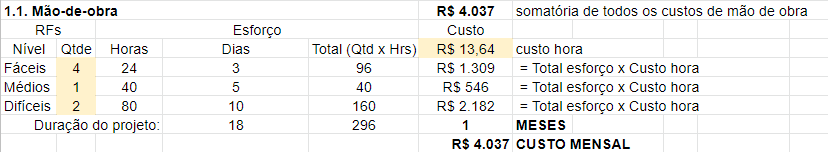
\includegraphics[width=1\textwidth]{images/Mao-de-obra.png}
                \caption{\DIFaddFL{Mão de obra}}
                \label{fig:infra}
            \end{figure}

            \DIFaddend \item \DIFdelbegin \DIFdel{Scrum Master: R\$ 2.500, }\DIFdelend \DIFaddbegin \DIFadd{Custo-base: R\$ 2.400,}\DIFaddend 00
            \DIFdelbegin \DIFdel{+ encargos de folha }\DIFdelend \item \DIFdelbegin \DIFdel{Team Member: R\$ 2.500, 00 + encargos de folha
    }%DIFDELCMD < \end{itemize}
%DIFDELCMD <     %%%
\DIFdelend \DIFaddbegin \DIFadd{Dias-base: 22 | Dia-hora: 8
            }\item \DIFadd{Custo-hora R\$ 13,64
}\DIFaddend 

        \DIFdelbegin \DIFdel{Considerando que os encargos de folha são frequentemente aproximados a 100\% do valor bruto da remuneração, foi aplicado essa regra geral para facilitar o cálculo.
    }\DIFdelend %DIF >  \subsection{Destino dos Custos}

        \DIFdelbegin \DIFdel{Portanto, os custos de remuneração são de aproximadamente R\$ 36.000,00.
    }\DIFdelend %DIF >      Considerando as funcionalidades do projeto e o número de colaboradores, foram distribuídas tarefas para contabilizar as horas do projeto.

        \DIFdelbegin \subsection{\DIFdel{Tributação}}
    %DIFAUXCMD
\addtocounter{subsection}{-1}%DIFAUXCMD
\DIFdel{Impostos sobre serviços prestados com fato gerador ocorrido no município de São Paulo incide alíquota máxima para o imposto sobre serviço (ISS) , incorrendo 5\% do valor de faturamento.
 Demais tributações dependerão do regime tributário a ser escolhido na constituição jurídica, não sendo prevista no momento da elaboração do projeto.
    }\DIFdelend %DIF >      \begin{table*}[h]
        %DIF >          % \centering

        \DIFdelbegin %DIFDELCMD < \subsection{%%%
\DIFdel{Custos totais estimados}%DIFDELCMD < \MBLOCKRIGHTBRACE
%DIFDELCMD <     %%%
\DIFdel{Anualizando os valores e o câmbio fixado em 1 USD = 5,50 BRL, foi estimado custo anualizado das operações em R\$ 437.290,16, conforme demonstração}\DIFdelend %DIF >          \resizebox{\columnwidth}{80}{%
        %DIF >          \begin{tabular}{|lrrr|r|}
        %DIF >              \hline
        %DIF >              \multicolumn{1}{|l|}{Funcionalidade}                & \multicolumn{1}{r|}{Dias de Trabalho}
        %DIF >                  & \multicolumn{1}{r|}{Membros Atuando}
        %DIF >                  & \multicolumn{1}{r|}{Horas Totais}
        %DIF >                  &  Custo \\ \hline
        %DIF >              \multicolumn{1}{|l|}{Módulo de autenticação}
        %DIF >                  & \multicolumn{1}{r|}{3}
        %DIF >                  & \multicolumn{1}{r|}{2}
        %DIF >                  & \multicolumn{1}{r|}{48} 
        %DIF >                  & R\$ 654,55  \\ \hline
        %DIF >              \multicolumn{1}{|l|}{Agendamento online}           & \multicolumn{1}{r|}{3}
        %DIF >                  & \multicolumn{1}{r|}{2}
        %DIF >                  & \multicolumn{1}{r|}{48} 
        %DIF >                  & R\$ 654,55  \\ \hline
        %DIF >              \multicolumn{1}{|l|}{Prontuário clínico digital}
        %DIF >                  & \multicolumn{1}{r|}{10}
        %DIF >                  & \multicolumn{1}{r|}{6}
        %DIF >                  & \multicolumn{1}{r|}{480} 
        %DIF >                  & R\$ 6.545,45  \\ \hline
        %DIF >               \multicolumn{1}{|l|}{Registro de alterações assinadas digitalmente}
        %DIF >                  & \multicolumn{1}{r|}{10}
        %DIF >                  & \multicolumn{1}{r|}{3}
        %DIF >                  & \multicolumn{1}{r|}{240} 
        %DIF >                  & R\$ 3.272,73  \\ \hline
        %DIF >              \multicolumn{1}{|l|}{Gerenciamento de medicação}
        %DIF >                  & \multicolumn{1}{r|}{5}
        %DIF >                  & \multicolumn{1}{r|}{3}
        %DIF >                  & \multicolumn{1}{r|}{120} 
        %DIF >                  & R\$ 1.636,36  \\ \hline
        %DIF >              \multicolumn{1}{|l|}{Mapeamento Genealógico}
        %DIF >                  & \multicolumn{1}{r|}{3}
        %DIF >                  & \multicolumn{1}{r|}{3}
        %DIF >                  & \multicolumn{1}{r|}{72} 
        %DIF >                  & R\$ 981,82  \\ \hline
        %DIF >              \multicolumn{1}{|l|}{Controle de vacinação}
        %DIF >                  & \multicolumn{1}{r|}{3}
        %DIF >                  & \multicolumn{1}{r|}{3}
        %DIF >                  & \multicolumn{1}{r|}{72} 
        %DIF >                  & R\$ 981,82  \\ \hline
        %DIF >              \multicolumn{3}{|l|}{Total}
        %DIF >                  & \multicolumn{1}{r|}{1080}
        %DIF >                  & R\$ 14.727,27     \\ \hline
        %DIF >          \end{tabular}%
        %DIF >          }
        %DIF >          \caption{Destinação dos custos de desenvolvimento}
        %DIF >          \label{tab:custos_func}
        %DIF >      \end{table*}
\DIFaddbegin 

        \subsection{\DIFadd{Custos de Operação}}

            \DIFadd{Após o período de desenvolvimento, os custos para manter o projeto se devem exclusivamente a mensalidade dos servidores e da remuneração do Team Member responsável}\DIFaddend .


            %DIF <  Please add the following required packages to your document preamble:
    %DIF <  \usepackage{graphicx}
    \begin{table*}[ht]
    %DIF <  \centering
        \DIFdelbeginFL %DIFDELCMD < \resizebox{\columnwidth}{!}{%
%DIFDELCMD <         \begin{tabular}{|lrrrr|r|}
%DIFDELCMD <             \hline
%DIFDELCMD <             \multicolumn{1}{|l|}{Custo}                              & \multicolumn{1}{r|}{USD}   & \multicolumn{1}{r|}{Câmbio} & \multicolumn{1}{r|}{BRL}       & Quantidade & Total                            \\ \hline
%DIFDELCMD <             \multicolumn{1}{|l|}{Amazon CloudWatch}                  & \multicolumn{1}{r|}{1,21}  & \multicolumn{1}{r|}{5,50}   & \multicolumn{1}{r|}{6,655}     & 1          & 6,655                            \\ \hline
%DIFDELCMD <             \multicolumn{1}{|l|}{Amazon EC2}                         & \multicolumn{1}{r|}{13,44} & \multicolumn{1}{r|}{5,50}   & \multicolumn{1}{r|}{74,592}    & 1          & 74,592                           \\ \hline
%DIFDELCMD <             \multicolumn{1}{|l|}{Amazon RDS for MySQL}               & \multicolumn{1}{r|}{34,97} & \multicolumn{1}{r|}{5,50}   & \multicolumn{1}{r|}{192,335}   & 1          & 192,335                          \\ \hline
%DIFDELCMD <             \multicolumn{1}{|l|}{Amazon Simple Storage Service (S3)} & \multicolumn{1}{r|}{0,09}  & \multicolumn{1}{r|}{5,50}   & \multicolumn{1}{r|}{0,495}     & 1          & 0,495                            \\ \hline
%DIFDELCMD <             \multicolumn{1}{|l|}{Elastic Load Balancing}             & \multicolumn{1}{r|}{30,32} & \multicolumn{1}{r|}{5,50}   & \multicolumn{1}{r|}{166,76}    & 1          & 166,76                           \\ \hline
%DIFDELCMD <             \multicolumn{1}{|l|}{Product Owner}                      & \multicolumn{1}{r|}{}      & \multicolumn{1}{r|}{}       & \multicolumn{1}{r|}{3.000,00}  & 1          & 3.000,00                         \\ \hline
%DIFDELCMD <             \multicolumn{1}{|l|}{Scrum Master}                       & \multicolumn{1}{r|}{}      & \multicolumn{1}{r|}{}       & \multicolumn{1}{r|}{2.500,00}  & 1          & 2.500,00                         \\ \hline
%DIFDELCMD <             \multicolumn{1}{|l|}{Team Member}                        & \multicolumn{1}{r|}{}      & \multicolumn{1}{r|}{}       & \multicolumn{1}{r|}{2.500,00}  & 5          & 12.500,00                        \\ \hline
%DIFDELCMD <             \multicolumn{1}{|l|}{Encargos de Folha}                  & \multicolumn{1}{r|}{}      & \multicolumn{1}{r|}{}       & \multicolumn{1}{r|}{18.000,00} & 1          & 18.000,00                        \\ \hline
%DIFDELCMD <             \multicolumn{5}{|l|}{Total Mensal}                                                                                                                                & 36.440.847                       \\ \hline
%DIFDELCMD <             \multicolumn{5}{|l|}{Total Anual}                                                                                                                                 & \multicolumn{1}{l|}{437.290,164} \\ \hline
%DIFDELCMD <         \end{tabular}%
%DIFDELCMD <         }
%DIFDELCMD <     %%%
\DIFdelendFL \DIFaddbeginFL \resizebox{\columnwidth}{!}{%
    \begin{tabular}{|lrrrr|r|}
        \hline
        \multicolumn{1}{|l|}{Custo}                              & \multicolumn{1}{r|}{USD}   & \multicolumn{1}{r|}{Câmbio} & \multicolumn{1}{r|}{BRL}       & Quantidade & Total                            \\ \hline
        \multicolumn{1}{|l|}{Amazon CloudWatch}                  & \multicolumn{1}{r|}{1,21}  & \multicolumn{1}{r|}{5,50}   & \multicolumn{1}{r|}{6,655}     & 1          & 6,66                            \\ \hline
        \multicolumn{1}{|l|}{Amazon EC2}                         & \multicolumn{1}{r|}{13,44} & \multicolumn{1}{r|}{5,50}   & \multicolumn{1}{r|}{74,592}    & 1          & 74,59                           \\ \hline
        \multicolumn{1}{|l|}{Amazon RDS for MySQL}               & \multicolumn{1}{r|}{34,97} & \multicolumn{1}{r|}{5,50}   & \multicolumn{1}{r|}{192,335}   & 1          & 192,34                          \\ \hline
        \multicolumn{1}{|l|}{Amazon Simple Storage Service (S3)} & \multicolumn{1}{r|}{0,09}  & \multicolumn{1}{r|}{5,50}   & \multicolumn{1}{r|}{0,495}     & 1          & 0,50                            \\ \hline
        \multicolumn{1}{|l|}{Elastic Load Balancing}             & \multicolumn{1}{r|}{30,32} & \multicolumn{1}{r|}{5,50}   & \multicolumn{1}{r|}{166,76}    & 1          & 166,76                           \\ \hline
        \multicolumn{1}{|l|}{Team Member}                        & \multicolumn{1}{r|}{}      & \multicolumn{1}{r|}{}       & \multicolumn{1}{r|}{2.400,00}  & 1          & 2.400,00                        \\ \hline
        \multicolumn{5}{|l|}{Total Mensal}                                                                                                                                & 2.840,85                       \\ \hline
        \multicolumn{5}{|l|}{Total Anual}                                                                                                                                 & \multicolumn{1}{l|}{34.090,20} \\ \hline
    \end{tabular}%
    }
\caption{\DIFaddFL{Custos Totais Estimados}}
\label{tab:custos}
\DIFaddendFL \end{table*}

        \DIFdelbegin \chapter[Desenvolvimento]{\DIFdel{Desenvolvimento}}
    %DIFAUXCMD
\addtocounter{chapter}{-1}%DIFAUXCMD
\DIFdel{Tratando das metodologias de gestão para o projeto e ferramentas que serão utilizadas.
}\DIFdelend \DIFaddbegin \subsection{\DIFadd{Receitas}}
            \begin{table}[H]
                \resizebox{\columnwidth}{!}{%
                \begin{tabular}{| p{5cm}|l|l|l|}
                    \hline
                    \multicolumn{1}{|c|}{} & \multicolumn{1}{|c|}{\textbf{Plano Básico  R\$110,00/mês}}  & \multicolumn{1}{c|}{\textbf{Plano Premium  R\$ 165,00/mês}} \\ \hline
                    Agenda  &x &x \\ \hline

                    Prontuário Clínico   &x &x\\ \hline

                    Controle de Vacinação &x &x \\ \hline

                    Gerenciador de Medicamentos &x &x \\ \hline

                    Rastreio de Alterações &   &x  \\ \hline

                    Mapeamentos Genealógico &  &x \\ \hline
                \end{tabular}%
                }
            \caption{\DIFaddFL{Captação de Recursos}}
            \label{tab:custos}
            \end{table}
            \DIFaddend 

            \DIFdelbegin \section{\DIFdel{Metodologias}}
%DIFAUXCMD
\addtocounter{section}{-1}%DIFAUXCMD
\DIFdelend \DIFaddbegin \begin{figure}[H]
                \centering
                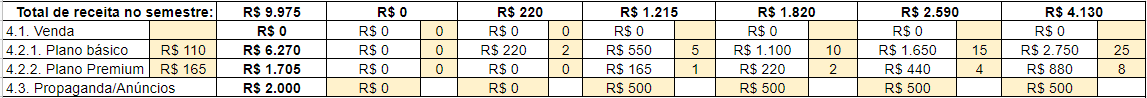
\includegraphics[width=1 \textwidth]{images/REALISTA.png}
                \caption{\DIFaddFL{Cenário Realista}}
                \label{fig:grafico pet}
            \end{figure}
    \DIFaddend 

        \DIFdelbegin \subsection{\DIFdel{Gestão de projeto}}
    %DIFAUXCMD
\addtocounter{subsection}{-1}%DIFAUXCMD
\DIFdel{Partindo de um estudo das necessidades da equipe e do projeto, ao considerar a necessidade mutável dos requisitos do mesmo e o cronograma restrito que foi definido, é vantajoso adotar uma combinação entre as metodologias Scrum (SCHWABER, 1993) e XP (WELLS, 1999), utilizando do XP de forma complementar ao Scrum, somando os processos de engenharia e desenvolvimento de software do primeiro com os rituais que dinamizam o desenvolvimento do segundo, fomentando entregas rápidas e incrementais.
    }\DIFdelend \DIFaddbegin \subsection{\DIFadd{Cenário Realista}}
            \begin{figure}[H]
                \centering
                \includegraphics[width=1 \textwidth]{images/CenárioRealista.png}
                \caption{\DIFaddFL{Cenário Realista}}
                \label{fig:grafico pet}
            \end{figure}
\DIFaddend 

    \DIFdelbegin \DIFdel{Os ciclos para o desenvolvimento do projeto são com duração de uma semana, as Sprints, a fim de conseguir focar durante esse período e ter maior controle dos prazos de entrega, além de definir o Product Backlog, criando um conjunto de funcionalidades a serem desenvolvidas no projeto para atingir o objetivo principal da aplicação. Ao final de cada Sprint a equipe se reunirá para discutir o que fora concluído, quais os resultados obtidos e avaliar o que correu bem durante a semana, criando um debate em cima dos problemas encontrados com a prática de Sprint Review. E também planejar a Sprint da semana seguinte, a fim de priorizar os itens do backlog a serem trabalhados para a próxima entrega, como nas Sprint Plannings.
    }\DIFdelend \DIFaddbegin \section{\DIFadd{Fases de entrega}}
    \DIFaddend 

        \DIFdelbegin \DIFdel{A prática de pair programing é algo que será adotado a fim de estimular o perfil colaborativo do time, permitindo um maior compartilhamento dos conhecimentos de cada um}\DIFdelend \DIFaddbegin \DIFadd{O desenvolvimento do projeto foi dividido em três fases de entregas recorrentes}\DIFaddend , de forma que \DIFdelbegin \DIFdel{impeça possíveis atrasos no desenvolvimento decorrentes de dúvidas ou travas pessoais, implicando em uma equipe de alto desempenho. Com isso, somado está a iniciativa de código colaborativo a fim de conquistar uma responsabilidade de forma generalizada no time, ou seja, o código }\DIFdelend \DIFaddbegin \DIFadd{atendesse à demanda recebida por parte dos clientes. A primeira delas consiste na POC, a segunda a apresentação do MVP e, para finalizar, a Entrega Final. A tabela a seguir relaciona as principais funcionalidades da CertVet com a fase em que a sua implementação }\DIFaddend é \DIFdelbegin \DIFdel{de propriedade coletiva onde todos devem possuir autonomia para modificações, de forma que não seja individualizada qualquer responsabilidade, aumentando o conhecimento da equipe e fomentando o compartilhamento e comunicação entre os integrantes.
    }\DIFdelend \DIFaddbegin \DIFadd{esperada.
    }\DIFaddend 

        \DIFdelbegin \DIFdel{A fim de organizar melhor a equipe, foi decidido seguir uma hierarquia de responsabilidades pensando na eficácia do desenvolvimento do projeto, discutindo sobre os cargos de Product Owner, Scrum Master e Rocket Members. }%DIFDELCMD < 

%DIFDELCMD <     %%%
\DIFdel{A função de PO (Product Owner) ficou com a cargo da Irina Chang, tendo como principal objetivo representar os interesses dos stakeholders, agregando valor ao negócio de forma a definir as funcionalidades do produto e fazendo a gestão do backlog, de acordo com o que deve ser priorizado, segundo as metodologias ágeis adotadas.
    }\DIFdelend \DIFaddbegin \subsubsection{\DIFadd{Escopo do projeto}}
            \begin{table}[H]
                \centering
                \resizebox{\columnwidth}{!}{%
                \begin{tabular}{|lrrrr|r|}
                    \hline
                    \multicolumn{1}{|l|}{Funcionalidades}                              & \multicolumn{1}{r|}{POC}   & \multicolumn{1}{r|}{MVP} & \multicolumn{1}{r|}{Produto Final}                                   \\ \hline\multicolumn{1}{|l|}{Processo de login}                  & \multicolumn{1}{c|}{X}  & \multicolumn{1}{c|}{X}   & \multicolumn{1}{c|}{X}                                 \\ \hline
                    \multicolumn{1}{|l|}{Módulo de autenticação}                  & \multicolumn{1}{c|}{}  & \multicolumn{1}{c|}{X}   & \multicolumn{1}{c|}{X}                                 \\ \hline
                    \multicolumn{1}{|l|}{Agendamento online}                         & \multicolumn{1}{c|}{} & \multicolumn{1}{c|}{X}   & \multicolumn{1}{c|}{X}                               \\ \hline
                    \multicolumn{1}{|l|}{Prontuário clínico digital}               & \multicolumn{1}{r|}{} & \multicolumn{1}{c|}{X}   & \multicolumn{1}{c|}{X}                             \\ \hline
                    \multicolumn{1}{|l|}{Registro de alterações assinados digitalmente} & \multicolumn{1}{r|}{}  & \multicolumn{1}{r|}{}   & \multicolumn{1}{c|}{X}                                 \\ \hline
                    \multicolumn{1}{|l|}{Gerenciamento de medicação}             & \multicolumn{1}{r|}{} & \multicolumn{1}{r|}{}   & \multicolumn{1}{c|}{X}                               \\ \hline
                    \multicolumn{1}{|l|}{Mapeamento genealógico}                      & \multicolumn{1}{r|}{}      & \multicolumn{1}{r|}{}       & \multicolumn{1}{c|}{X}                           \\ \hline
                    \multicolumn{1}{|l|}{Controle de vacinação}                       & \multicolumn{1}{r|}{}      & \multicolumn{1}{r|}{}       & \multicolumn{1}{c|}{X}                           \\ \hline                  
                \end{tabular}%
                }
            \caption{\DIFaddFL{Escopo do Projeto}}
            \label{tab:escopo}
            \end{table}
        \DIFaddend 

        \DIFdelbegin \DIFdel{Assumindo o cargo de Scrum Master, moste Henrique Hiromi, sendo o principal responsável por garantir que os valores e práticas das metodologias adotadas estejam sendo seguidas como o planejado. Também monitora as tarefas desenvolvidas na sprint assegurando que sejam entregues com sucesso e garantindo que o time esteja sendo funcional e produtivo.
    }\DIFdelend \DIFaddbegin \subsubsection{\DIFadd{Prova de Conceito}}
        \DIFaddend 

            \DIFdelbegin \DIFdel{Rocket Member é a forma como foi decidido nomear os desenvolvedores, esses serão os responsáveis pela implementação de código, padronização de commits, integrações, modelagem de banco de dados, além de verificar se as alterações propostas pelo PO são viáveis e, caso sim, como devem ser feitas, por consequência, são os maiores responsáveis em relação }\DIFdelend \DIFaddbegin \DIFadd{A Prova de Conceito, POC, consiste na comprovação de viabilidade técnica da arquitetura proposta, sem considerar implementação de lógica de negócios. Oferece ao cliente uma demonstração de que o produto pode ser desenvolvido, visualizando uma }\DIFaddend a \DIFdelbegin \DIFdel{documentação do código de forma que garanta a sua alta manutenibilidade, auxiliando tanto as manutenções futuras quanto a colocar a }\DIFdelend \DIFaddbegin \DIFadd{ideia abstrata de como a }\DIFaddend aplicação \DIFdelbegin \DIFdel{em produção sem grandes problemas.
    Os rocket members são: Caique Daniel, Luis Renato, Marcos Querino, Murilo Pires e Welen Mota.
    }\DIFdelend \DIFaddbegin \DIFadd{se comporta. 
}\DIFaddend 

            \DIFdelbegin %DIFDELCMD < \begin{center}
%DIFDELCMD <     %%%
\DIFdel{Tabela de Membros
    }%DIFDELCMD < 

%DIFDELCMD <         \begin{tabulary}{1.0\textwidth}{|C|C|}
%DIFDELCMD <         \hline
%DIFDELCMD <          %%%
\DIFdel{Membro }%DIFDELCMD < & %%%
\DIFdel{Cargo }%DIFDELCMD < \\
%DIFDELCMD <         \hline
%DIFDELCMD <         %%%
\DIFdel{Irina Chang }%DIFDELCMD < & %%%
\DIFdel{Product Owner}%DIFDELCMD < \\
%DIFDELCMD <         \hline
%DIFDELCMD <         %%%
\DIFdel{Henrique Hiromi }%DIFDELCMD < & %%%
\DIFdel{Scrum Master}%DIFDELCMD < \\
%DIFDELCMD <         \hline
%DIFDELCMD <         %%%
\DIFdel{Caique Daniel }%DIFDELCMD < & %%%
\DIFdel{Rocket Member}%DIFDELCMD < \\
%DIFDELCMD <         \hline
%DIFDELCMD <         %%%
\DIFdel{Luis Renato }%DIFDELCMD < & %%%
\DIFdel{Rocket Member}%DIFDELCMD < \\
%DIFDELCMD <         \hline
%DIFDELCMD <         %%%
\DIFdel{Marcos Querino }%DIFDELCMD < & %%%
\DIFdel{Rocket Member}%DIFDELCMD < \\
%DIFDELCMD <         \hline
%DIFDELCMD <         %%%
\DIFdel{Murilo Santos }%DIFDELCMD < & %%%
\DIFdel{Rocket Member}%DIFDELCMD < \\
%DIFDELCMD <         \hline
%DIFDELCMD <         %%%
\DIFdel{Wellen Mota }%DIFDELCMD < & %%%
\DIFdel{Rocket Member}%DIFDELCMD < \\
%DIFDELCMD <         \hline
%DIFDELCMD <         \end{tabulary}
%DIFDELCMD <     \end{center}
%DIFDELCMD < 

%DIFDELCMD <     %%%
\subsection{\DIFdel{Ferramentas de gestão}}
    %DIFAUXCMD
\addtocounter{subsection}{-1}%DIFAUXCMD
\DIFdel{As ferramentas utilizadas são: plataforma GitHub para compartilhamento de documentos, Google Meet para as reuniões semanais de definição e alinhamento do escopo da Sprint, WhatsApp para troca de mensagens urgentes e o Jira para distribuição e controle das tarefas. 
}%DIFDELCMD < 

%DIFDELCMD < %%%
\chapter{\DIFdel{Análise de concorrência}}
%DIFAUXCMD
\addtocounter{chapter}{-1}%DIFAUXCMD
%DIFDELCMD < 

%DIFDELCMD < %%%
\DIFdel{A fim de comparação, foram selecionadas as principais aplicações já presentes no mercado que atuam na mesma problemática da Sidekick. }%DIFDELCMD < 

%DIFDELCMD < %%%
\section{\DIFdel{Tabela comparativa}}
%DIFAUXCMD
\addtocounter{section}{-1}%DIFAUXCMD
%DIFDELCMD < \begin{center}
%DIFDELCMD <     %%%
\DIFdel{Tabela Comparativa
    }%DIFDELCMD < \begin{tabulary}{1.0\textwidth}{|L|L|L|L|L|L|L|L|L|}
%DIFDELCMD <     \hline
%DIFDELCMD <      & %%%
\DIFdel{Sidekick }%DIFDELCMD < & %%%
\DIFdel{Simples Vet }%DIFDELCMD < & %%%
\DIFdel{Vet work }%DIFDELCMD < & %%%
\DIFdel{Doctor Vet }%DIFDELCMD < & %%%
\DIFdel{Dr. Snoopy Smart }%DIFDELCMD < & %%%
\DIFdel{Vet soft }%DIFDELCMD < & %%%
\DIFdel{Beans Vet}%DIFDELCMD < \\
%DIFDELCMD <     \hline
%DIFDELCMD <     %%%
\DIFdel{Agenda }%DIFDELCMD < & %%%
\DIFdel{x }%DIFDELCMD < & %%%
\DIFdel{x }%DIFDELCMD < & %%%
\DIFdel{x }%DIFDELCMD < & %%%
\DIFdel{x }%DIFDELCMD < & %%%
\DIFdel{x }%DIFDELCMD < & %%%
\DIFdel{x }%DIFDELCMD < & %%%
\DIFdel{x}%DIFDELCMD < \\
%DIFDELCMD <     \hline
%DIFDELCMD <     %%%
\DIFdel{Rastreio de alterações }%DIFDELCMD < & %%%
\DIFdel{x }%DIFDELCMD < &  &  &  &  &  & \\
%DIFDELCMD <     \hline
%DIFDELCMD <     %%%
\DIFdel{Gerenciamento de medicação }%DIFDELCMD < & %%%
\DIFdel{x }%DIFDELCMD < & %%%
\DIFdel{x }%DIFDELCMD < &  & %%%
\DIFdel{x }%DIFDELCMD < & %%%
\DIFdel{x }%DIFDELCMD < & %%%
\DIFdel{x }%DIFDELCMD < & %%%
\DIFdel{x}%DIFDELCMD < \\
%DIFDELCMD <     \hline
%DIFDELCMD <     %%%
\DIFdel{Prontuário clínico }%DIFDELCMD < & %%%
\DIFdel{x }%DIFDELCMD < & %%%
\DIFdel{x }%DIFDELCMD < & %%%
\DIFdel{x }%DIFDELCMD < & %%%
\DIFdel{x }%DIFDELCMD < & %%%
\DIFdel{x }%DIFDELCMD < & %%%
\DIFdel{x }%DIFDELCMD < & %%%
\DIFdel{x}%DIFDELCMD < \\
%DIFDELCMD <     \hline
%DIFDELCMD <     %%%
\DIFdel{Mapeamento genealógico }%DIFDELCMD < & %%%
\DIFdel{x }%DIFDELCMD < &  &  &  &  &  & \\
%DIFDELCMD <     \hline
%DIFDELCMD <     %%%
\DIFdel{Controle de vacinação }%DIFDELCMD < & %%%
\DIFdel{x }%DIFDELCMD < &  &  & %%%
\DIFdel{x }%DIFDELCMD < & %%%
\DIFdel{x }%DIFDELCMD < & %%%
\DIFdel{x }%DIFDELCMD < & %%%
\DIFdel{x}%DIFDELCMD < \\
%DIFDELCMD <     \hline
%DIFDELCMD <     \end{tabulary}
%DIFDELCMD < \end{center}
%DIFDELCMD < 

%DIFDELCMD < %%%
\section{\DIFdel{SimplesVet}}
%DIFAUXCMD
\addtocounter{section}{-1}%DIFAUXCMD
\DIFdel{O SimplesVet se apresenta como um sistema para petshop e clínica veterinária que busca ajudar a simplificar a rotina da clínica. Consiste em um sistema acessado via WEB, permitindo o controle da clínica a qualquer hora ou lugar, contanto que tenha acesso a internet. Suas funcionalidades dividem-se em:
}%DIFDELCMD < 

%DIFDELCMD < \begin{itemize}
%DIFDELCMD <     

%DIFDELCMD <     \item %%%
\DIFdel{Atendimento veterinário: permite o registro das fichas veterinárias em uma tela simples, com dados salvos na nuvem.
    }%DIFDELCMD < \item %%%
\DIFdel{Agenda de serviços: possibilita a organização da agenda dos veterinários e envia lembretes sobre os próximos atendimentos.
    }%DIFDELCMD < \item %%%
\DIFdel{Internação veterinária: organização dos prontuários e agendas de plantão.
    }%DIFDELCMD < \item %%%
\DIFdel{Controle financeiro: possibilita a organização do fluxo de caixa da clínica e envia lembretes de contas a pagar no celular cadastrado. 
}%DIFDELCMD < \item %%%
\DIFdel{Gestão de estoque: visualização dos produtos a repor, itens próximos ao vencimento, produtos parados e etc.
    }%DIFDELCMD < \item %%%
\DIFdel{Análise de vendas: visualização de um dashboard voltado }\DIFdelend \DIFaddbegin \DIFadd{Para a POC da CertVet, a equipe apresentou o desenho da arquitetura com as especificações propostas sendo um processo de cadastro de usuário e login e regras de negócio simples implementadas no back end. Este processo teve a finalidade de demonstrar o trânsito dos dados através de chamadas com sucesso }\DIFaddend à \DIFdelbegin \DIFdel{estratégias de marketing, listando produtos mais vendidos, ticket médio, horários de pico e etc.
    }%DIFDELCMD < \item %%%
\DIFdel{Notas fiscais: emissão de notas fiscais de produto (NFC-e), serviço (NFS-e) e nota grande (NF-e).
    }%DIFDELCMD < \item %%%
\DIFdel{App para tutores: um app feito para o cliente com datas de vacinação, exames e informações do pet.
    }%DIFDELCMD < \item %%%
\DIFdel{Mensagens automáticas: envio de lembrete de consultas e vacinas para os tutores e agenda para veterinários}\DIFdelend \DIFaddbegin \DIFadd{API implementada no servidor com respostas previamente esperadas, demonstrando a comunicação entre as camadas foi realizada com sucesso}\DIFaddend .
    \DIFdelbegin %DIFDELCMD < \item %%%
\DIFdel{SMS Marketing: envio de campanhas via SMS para os clientes. }%DIFDELCMD < \item %%%
\DIFdel{Pesquisa e satisfação: possibilita o recebimento de avaliações dos clientes para fins comparativos com o mercado.
}%DIFDELCMD < \end{itemize}
%DIFDELCMD < %%%
\DIFdelend 

        \DIFdelbegin \DIFdel{A SimplesVet possui mais features voltadas }\DIFdelend \DIFaddbegin \subsubsection{\DIFadd{Produto Mínimo Viável}}

            \DIFadd{O MVP entregue na segunda fase consiste em uma primeira versão da aplicação com as funcionalidades essenciais identificadas pela análise do grupo junto }\DIFaddend à \DIFdelbegin \DIFdel{gerência de assuntos de PetShop, como controle de estoque e de vendas, cumprindo de forma básica apenas uma das demandas da clínica veterinária. Enquanto a Sideckick tem como principal objetivo resolver de forma simples as demandas do ambiente clínico, voltadas principalmente ao trabalho realizado pelo veterinário, como: manutenção de prontuário digital, controle de internação, controle da medicação e da autenticação de receitas, dentre outras, resolvendo demandas que não são contempladas pelo SimplesVet.
}\DIFdelend \DIFaddbegin \DIFadd{profissional devidamente habilitada e praticante.
            }\DIFaddend 

            \DIFdelbegin \section{\DIFdel{Vetwork}}
%DIFAUXCMD
\addtocounter{section}{-1}%DIFAUXCMD
\DIFdel{O Vetwork destaca-se entre os usuários pela sua interface intuitiva sendo algo que auxilia na produtividade do trabalho, trata-se de um sistema de gestão baseado na nuvem, não fazendo necessária }\DIFdelend \DIFaddbegin \DIFadd{Após }\DIFaddend a \DIFdelbegin \DIFdel{instalação de hardware ou software, pois funciona nativo SaaS. Seus 2.744 usuários dispõem das seguintes funcionalidades:
}\DIFdelend \DIFaddbegin \DIFadd{liberação do MVP, será possível adicionar novas funcionalidades a partir do feedbacks dos usuários e implementação de funcionalidades previamente planejadas.
            }\DIFaddend 

            \DIFdelbegin %DIFDELCMD < \begin{itemize}
%DIFDELCMD <     \item %%%
\DIFdel{Agenda vinculada ao caixa: um controle geral das atividades realizadas nos pets, como consultas médicas, retornos, exames, cirurgias, banhos, tosas e todos os outros procedimentos, sem limite de datas.
    }%DIFDELCMD < \item %%%
\DIFdel{Gestão de Documentos: permite a inclusão de documentos e arquivos à ficha clínica do animal, como laudos, fotografias, exames de imagem e outros, que são armazenados na internet e podem ser acessados de qualquer lugar.
    }%DIFDELCMD < \item %%%
\DIFdel{Calendário: uma forma de controle das datas e horários em que os animais passaram por procedimentos como banhos, tosas, exames, consultas, vacinas ou quaisquer outros realizados no estabelecimento.
    }%DIFDELCMD < \item %%%
\DIFdel{Gestão clínica: }\DIFdelend \DIFaddbegin \DIFadd{A CertVet contempla em seu MVP, além dos processos de cadastro e login, a melhoria do módulo de autenticação do usuário, o serviço de agendamento on-line e a }\DIFaddend criação \DIFaddbegin \DIFadd{e manutenção }\DIFaddend de prontuário \DIFdelbegin \DIFdel{eletrônico com as informações médicas do pet, como controle de registros clínicos, exames, vacinas e doses adicionais.
            }%DIFDELCMD < \item %%%
\DIFdel{Gestão Financeira: controle de caixa, pacotes, contas a pagar e a receber, pagamentos pendentes e pré-vendas, cálculo de comissionamento e geração de relatórios financeiros da empresa.
            }%DIFDELCMD < \item %%%
\DIFdel{Relacionamento com o Cliente: armazenamento de todas as informações dos clientes para possibilitar um relacionamento mais próximo com o mesmo.
    }%DIFDELCMD < \item %%%
\DIFdel{E-mail Inclusos: mensagens automáticas, através de e-mail, para comunicação instantânea.
}%DIFDELCMD < \end{itemize}
%DIFDELCMD < 

%DIFDELCMD < %%%
\DIFdel{Apesar de ser uma aplicação mais completa em relação à anterior, ainda assim o prontuário eletrônico é o ponto forte desse serviço, no que tange à funcionalidades para o fluxo }\DIFdelend clínico \DIFdelbegin \DIFdel{veterinário. A Sidekick busca resolver de forma eficaz e mais completa, o controle de medicamentos, não só o seu cadastro e quantidade em estoque, mas o uso de uma chave de autenticação para receitas e a aplicação dos mesmos. De forma resumida, o Vetwork é sim uma ferramenta bem útil mas a aplicação aqui proposta resolve demandas que não são resolvidas por esse serviço, por mais que suas avaliações no mercado sejam positivas.
}\DIFdelend \DIFaddbegin \DIFadd{digital.
        }\DIFaddend 

        \DIFdelbegin \section{\DIFdel{DoctorVet}}
%DIFAUXCMD
\addtocounter{section}{-1}%DIFAUXCMD
\DIFdel{O DoctorVet é um sistema totalmente voltado à gestão de clínicas e hospitais veterinários e apresenta duas versões: uma standard com módulos para controle de consultas, vacinas, pequenas cirurgias, assuntos de pet shop e também financeiro. E uma versão enterprise que contempla todos os módulos standard e adicionalmente um controle de internação e hospedagem e concentra informações do centro cirúrgico e laboratório.  Funcionalidades da versão Enterprise do DoctorVet:
}\DIFdelend \DIFaddbegin \subsubsection{\DIFadd{Produto Final}}
        \DIFaddend 

            \DIFdelbegin %DIFDELCMD < \begin{itemize}
%DIFDELCMD <     \item %%%
\DIFdel{Módulo de Cadastro: realiza o cadastro de veterinários, funcionários, animais, clientes e planos de atendimento.
    }%DIFDELCMD < \item %%%
\DIFdel{Módulo Farmacológico: permite o cadastro de vacinas, vermífugos e o cadastro de procedimentos ou interações medicamentosas.
    }%DIFDELCMD < \item %%%
\DIFdel{Módulo Atendimento: criação de ficha de atendimento, lista de espera, curadoria de orçamentos, central de   agendamentos e controle de status do veterinário.
    }%DIFDELCMD < \item %%%
\DIFdel{Módulo Caixa: utilizado pelos atendentes de caixa, controle das formas de recebimento, abertura e fechamento do caixa e manutenção.
    }%DIFDELCMD < \item %%%
\DIFdel{Módulo Consultório: consultas generalistas e especialistas, histórico de consultas e atendimentos, pedidos de exames, receituários e prontuário eletrônico.
        }%DIFDELCMD < \item %%%
\DIFdel{Módulo Pet Shop: permite televendas, consulta de preços e relatórios e emissão de cupom fiscal.
    }%DIFDELCMD < \item %%%
\DIFdel{Módulo Internação Básica/ Avançada: admissão }\DIFdelend \DIFaddbegin \DIFadd{A partir da finalização do MVP, será possível adicionar as funcionalidades de registro de alterações assinados digitalmente pelo veterinário, gerenciamento }\DIFaddend de \DIFdelbegin \DIFdel{internação, controle da evolução do quadro clínico, alta veterinária, manter prontuários, cadastro de prescrições.
    }%DIFDELCMD < \item %%%
\DIFdel{Módulo Estoque: cadastro de fornecedores, cadastro e etiquetação de produtos, gerenciamento de lotes, requisições à farmácia e requisições internas}\DIFdelend \DIFaddbegin \DIFadd{medicação controlada, permitir mapeamento genealógico dos animais}\DIFaddend , controle de \DIFdelbegin \DIFdel{compras e relatórios.
    }%DIFDELCMD < \item %%%
\DIFdel{Módulo Exames: controle de exames laboratoriais e seus resultados.
    }%DIFDELCMD < \item %%%
\DIFdel{Módulo Laboratório: cadastros, central de coleta e composição de exames.
}%DIFDELCMD < \item %%%
\DIFdel{Módulo Centro Diagnóstico: preparo para exames e suas composições.
    }%DIFDELCMD < \item %%%
\DIFdel{Módulo Relatórios: criação de relatórios operacionais, gerenciais e estratégicos (CRM, SPED Fiscal e Pis, Cofins)
    }%DIFDELCMD < \item %%%
\DIFdel{Módulo Segurança: cadastro de usuários e permissões de acesso de acordo com níveis.
}%DIFDELCMD < \end{itemize}
%DIFDELCMD < 

%DIFDELCMD < %%%
\DIFdel{É a aplicação mais recente das selecionadas e também a mais completa, no entanto, reforça-se aqui que não contempla o controle de medicamentos, oferecido pela Sideckick.
}%DIFDELCMD < 

%DIFDELCMD < %%%
\section{\DIFdel{Dr. Snoopy Smart}}
%DIFAUXCMD
\addtocounter{section}{-1}%DIFAUXCMD
\DIFdel{O Dr. Snoopy Smart se apresenta como um sistema completo de gestão exclusivo para Pet Shop e clínicas veterinárias, automatizando processos clínicos, na tentativa de agilizar as tarefas e tendo o aumento das vendas como foco do módulo de pet shop. Consiste em um software com as seguintes funcionalidades:
}%DIFDELCMD < 

%DIFDELCMD < \begin{itemize}
\begin{itemize}%DIFAUXCMD
%DIFDELCMD <     \item %%%
\item%DIFAUXCMD
\DIFdel{Agendamento otimizado: permitindo o controle de agendamento dos pacientes.
    }%DIFDELCMD < \item %%%
\item%DIFAUXCMD
\DIFdel{Gerenciamento de estoque: visibilidade da quantidade de produtos e quais estão em falta.
    }%DIFDELCMD < \item %%%
\item%DIFAUXCMD
\DIFdel{Prontuário Clínico: possibilita a criação e consulta da ficha veterinária dos animais.
    }%DIFDELCMD < \item %%%
\item%DIFAUXCMD
\DIFdel{Emissão de Notas: emissão de NF-e, NFS-e e Cupons Fiscais.
    }%DIFDELCMD < \item %%%
\item%DIFAUXCMD
\DIFdel{Histórico de Pacientes: arquivação e consulta de informações dos atendimentos. 
    }%DIFDELCMD < \item %%%
\item%DIFAUXCMD
\DIFdel{Vacinas sempre em dia: controle de quando o paciente deve ser vacinado.
    }%DIFDELCMD < \item %%%
\item%DIFAUXCMD
\DIFdel{Agenda de Banho e Tosa: específica para tais, permitindo um maior controle do pet shop. }%DIFDELCMD < \item %%%
\item%DIFAUXCMD
\DIFdel{Gestão Integrada: permite acessar à determinados indicadores de gestão.
    }%DIFDELCMD < \item %%%
\item%DIFAUXCMD
\DIFdel{Notificações SMS: recebimento de lembretes importantes no celular dos usuários da aplicação
    }%DIFDELCMD < \item %%%
\item%DIFAUXCMD
\DIFdel{Relatórios Personalizados: geração de relatórios com facilidade.
}
\end{itemize}%DIFAUXCMD
%DIFDELCMD < \end{itemize}
%DIFDELCMD < 

%DIFDELCMD < %%%
\DIFdel{Apesar de ser uma aplicação com muitas funcionalidades, ainda assim não apresenta as opções de modernidade que a aplicação aqui proposta oferece, haja vista que divide o escopo clínico com as necessidades de um pet shop, apresentando mais funcionalidades voltadas à gestão e estratégias de venda do que para o fluxo de trabalho do profissional }\DIFdelend \DIFaddbegin \DIFadd{vacinação e validação de autenticidade de documento do }\DIFaddend veterinário \DIFdelbegin \DIFdel{.
}\DIFdelend \DIFaddbegin \DIFadd{junto ao órgão de classe.
}\DIFaddend 

\DIFdelbegin \section{\DIFdel{Vetsoft}}
%DIFAUXCMD
\addtocounter{section}{-1}%DIFAUXCMD
\DIFdel{O programa VetSoft é oferecido nas versões Desktop e Web, sendo essa primeira uma versão instalada nos computadores em rede, permitindo o acesso mesmo com falta de conexão com a Internet. E a versão Web, um sistema em nuvem que permite ao usuário gerenciar o negócio através de diferentes dispositivos, como computador, smartphone, tablet, etc, contanto que tenha acesso à Internet.
O VetSoft abrange serviços de clínica veterinária, hospital veterinário, pet shop / banho e tosa e veterinários autônomos com as seguintes funcionalidades:
}\DIFdelend \DIFaddbegin \chapter[Considerações Finais]{\DIFadd{Considerações Finais}}
\DIFaddend 

    \DIFdelbegin %DIFDELCMD < \begin{itemize}
%DIFDELCMD <     \item %%%
\DIFdel{Ficha do Tutor: ficha cadastral da conta do tutor e seus animais, visibilidade do histórico de pagamentos e envio de e-mail individual.
    }%DIFDELCMD < \item %%%
\DIFdel{Ficha do Animal: ficha cadastral específica dos animais pacientes, álbum de fotos, agendamentos, agrupamento dos resultados de exames e histórico de vacinas e vermífugos.
    }%DIFDELCMD < \item %%%
\DIFdel{Histórico Clínico: anamnese, diagnóstico, laudo clínico, receituário normal e especial e exames.
    }%DIFDELCMD < \item %%%
\DIFdel{Gestão de Estoque: divisão de produtos por grupos, controle de produtos com estoque baixo, visibilidade dos produtos mais e menos vendidos e entrada de estoque manual e XML.
    }%DIFDELCMD < \item %%%
\DIFdel{Financeiro: controle de caixa diário e seu fluxo, demonstrativo de resultados por área, centro de custos, controle de planos para clientes mensalistas.
    }%DIFDELCMD < \item %%%
\DIFdel{Emissão Fiscal: possibilidade de emissão fiscal para todos os estados e todos os formatos: NFCe, SAT, MFe e PAF-ECF.
}%DIFDELCMD < \item %%%
\DIFdel{Farmácia/Materiais: controle de estoque de farmácia e materiais de uso interno.
    }%DIFDELCMD < \item %%%
\DIFdel{Imunizações: controle da aplicação de vacinas e vermífugos na ficha do animal com agendamentos e }\DIFdelend \DIFaddbegin \DIFadd{A acessibilidade de tecnologias em nuvem e emprego de tecnologias portáveis de containerização permitem que }\DIFaddend aplicações \DIFdelbegin \DIFdel{realizadas.
}%DIFDELCMD < \end{itemize}
%DIFDELCMD < 

%DIFDELCMD < %%%
\DIFdel{É uma das aplicações mais completas, no entanto, o controle de medicamentos oferecido não atinge o mesmo grau de segurança que a chave de autenticação para as receitas que a Sidekick oferece, assumindo um papel importante na modernização dessa autenticação nos dias atuais.
}%DIFDELCMD < 

%DIFDELCMD < %%%
\section{\DIFdel{BensVet}}
%DIFAUXCMD
\addtocounter{section}{-1}%DIFAUXCMD
\DIFdel{O BensVet se diferencia dos demais apresentados por se tratar de um }\DIFdelend \DIFaddbegin \DIFadd{sejam criadas e transportadas com mínimo de interferência para o mantenedor e seus clientes. Entretanto, ao utilizar soluções proprietárias, como o }\DIFaddend serviço \DIFdelbegin \DIFdel{que se divide em dois aplicativos, um para uso veterinário e um para uso dos tutores. O aplicativo para veterinários garante que o usuário poderá iniciar um atendimento a domicílio e conseguir  dar continuidade na clínica. E o aplicativo para tutores trata-se dos processos de envio  de promoções e alertas de retorno automáticos para os tutores, permitindo também a consulta de  informações sobre o animal e agendamento de atendimentos pelo app. As funcionalidades dividem-se em :
}\DIFdelend \DIFaddbegin \DIFadd{Amazon S3, é necessário considerar o tipo de comprometimento por vendor lock in que corre-se o risco de expor a aplicação.
}\DIFaddend 

    \DIFdelbegin %DIFDELCMD < \begin{itemize}
%DIFDELCMD <     \item %%%
\DIFdel{Agenda de atendimentos. }%DIFDELCMD < \item %%%
\DIFdel{Acompanhamento de medicações }\DIFdelend \DIFaddbegin \DIFadd{Em suma, as utilização e aproveitamento de recursos computacionais, principalmente em nuvem, }\DIFaddend na \DIFdelbegin \DIFdel{internação.
    }%DIFDELCMD < \item %%%
\DIFdel{Criação de fichas clínicas personalizadas.
    }%DIFDELCMD < \item %%%
\DIFdel{Notificar automaticamente consultas, retornos e vacinas aos clientes.
    }%DIFDELCMD < \item %%%
\DIFdel{Consultar históricos de animais e seus tutores.
    }%DIFDELCMD < \item %%%
\DIFdel{Controle dos comissionamentos de profissionais.
    }%DIFDELCMD < \item %%%
\DIFdel{Emitir Notas Fiscais referente a venda de produtos.
    }%DIFDELCMD < \item %%%
\DIFdel{Controle de estoque.
}%DIFDELCMD < \end{itemize}
%DIFDELCMD < 

%DIFDELCMD < %%%
\DIFdel{Trata-se de uma resolução que se aproxima bastante da Sidekick no que tange à proximidade do profissional veterinário, esteja ele numa clínica ou trabalhando de forma autônoma, no entanto, observamos aqui que o controle de medicamentos oferecido, mais uma vez, }\DIFdelend \DIFaddbegin \DIFadd{área de medicina veterinária faz-se }\DIFaddend não \DIFdelbegin \DIFdel{atinge o mesmo grau de segurança que a chave de autenticação aqui propostas, além da funcionalidade de mapeamento genealógico}\DIFdelend \DIFaddbegin \DIFadd{somente benéfica por eliminar o risco de perda de dados em mídias físicas e aumentar a velocidade de recuperação de dados importantes e sensíveis.
}

    \DIFadd{As normas que regulam as atividades médico-veterinárias, em especial sobre medicação controlada, podem sofrer alterações que nem sempre são acompanhadas pelo técnico no momento em que são publicadas. Uma ferramenta de gestão focada nesta atividade reduz o risco do negócio se enquadrar em uma situação de irregularidade}\DIFaddend .

\DIFdelbegin %DIFDELCMD < \postextual
%DIFDELCMD < %%%
\DIFdelend \DIFaddbegin \chapter[Links do Projeto]{\DIFadd{Links do Projeto}}
    %DIF >  no momento este tópico fica como capitulo, mas na entrega final ele vai virar um tópico do capitulo de métricas
    \begin{figure} [\DIFaddFL{htb!}]
        \centering
        
\includegraphics[width=0.3\textwidth]{qrcode/qrcode_GIT.png}
        \caption{\DIFaddFL{Link Repositório no Github}}
        \label{fig:qrcode_GIT}
    \end{figure}
    \DIFaddend 

    \DIFdelbegin %DIFDELCMD < \begin{center}
%DIFDELCMD <         \begin{table}[h]
%DIFDELCMD <         %%%
\DIFdelendFL \DIFaddbeginFL \begin{figure}[htb!]
        \DIFaddendFL \centering
        \DIFdelbeginFL %DIFDELCMD < \resizebox{16cm}{!}{%
%DIFDELCMD <             \begin{tabular}{|p {15}|rrrrrrrr|}
%DIFDELCMD <             \hline
%DIFDELCMD <             \multicolumn{1}{|c|}{Membro}      & \multicolumn{1}{c|}{Irina}   & \multicolumn{1}{r|}{Henrique} & \multicolumn{1}{r|}{Caique}       & \multicolumn{1}{r|}{Luís} &
%DIFDELCMD <             \multicolumn{1}{r|}{\begin{tabular}[c]{@{}c@{}}Marcos \end{tabular}}  &
%DIFDELCMD <             \multicolumn{1}{r|}{Murilo} & \multicolumn{1}{r|}{Welen}\\ \hline
%DIFDELCMD <                

%DIFDELCMD <     \multicolumn{1}{|l|}{\begin{tabular}[c]{@{}c@{}}Documentação \end{tabular}} &
%DIFDELCMD <          \multicolumn{1}{c|}{x}  & \multicolumn{1}{c|}{x}  & \multicolumn{1}{c|}{x}  & \multicolumn{1}{c|}{x}  & \multicolumn{1}{c|}{x}  & \multicolumn{1}{c|}{x}  & \multicolumn{1}{c|}{x}            \\ \hline
%DIFDELCMD <     \multicolumn{1}{|l|}{\begin{tabular}[c]{@{}c@{}}Front-end \end{tabular}}&                 
%DIFDELCMD <         \multicolumn{1}{c|}{ }  & \multicolumn{1}{c|}{ }  & \multicolumn{1}{c|}{ x }  & \multicolumn{1}{c|}{x}  & \multicolumn{1}{c|}{x}    & \multicolumn{1}{c|}{ }  & \multicolumn{1}{c|}{ }            \\ \hline
%DIFDELCMD <  

%DIFDELCMD <     \multicolumn{1}{|l|}{\begin{tabular}[c]{@{}c@{}}Back-end \end{tabular}} &
%DIFDELCMD <         \multicolumn{1}{c|}{x} & \multicolumn{1}{c|}{x}  & \multicolumn{1}{c|}{} & \multicolumn{1}{c|}{}  & \multicolumn{1}{c|}{} & \multicolumn{1}{c|}{x}  & \multicolumn{1}{c|}{}            \\ \hline
%DIFDELCMD <                   

%DIFDELCMD <   \multicolumn{1}{|l|}{\begin{tabular}[c]{@{}c@{}}Banco de dados \end{tabular}} &
%DIFDELCMD <         \multicolumn{1}{c|}{}  & \multicolumn{1}{c|}{}  & \multicolumn{1}{c|}{x} & \multicolumn{1}{c|}{}  & \multicolumn{1}{c|}{}  & \multicolumn{1}{c|}{}  & \multicolumn{1}{c|}{}            \\ \hline
%DIFDELCMD <   

%DIFDELCMD <     \multicolumn{1}{|l|}{\begin{tabular}[c]{@{}c@{}}Infraestrutura \end{tabular}} &
%DIFDELCMD <         \multicolumn{1}{c|}{ }  & \multicolumn{1}{c|}{x} & \multicolumn{1}{c|}{ } & \multicolumn{1}{c|}{ } & \multicolumn{1}{c|}{ } & \multicolumn{1}{c|}{ }  & \multicolumn{1}{c|}{ }            \\ \hline
%DIFDELCMD < 

%DIFDELCMD <    \end{tabular}%
%DIFDELCMD <        }
%DIFDELCMD <         %%%
\DIFdelendFL \DIFaddbeginFL 
\includegraphics [\DIFaddFL{width=0.3\textwidth}]{\DIFaddFL{qrcode/qrcode_YT.png}}
        \DIFaddendFL \caption{\DIFdelbeginFL \DIFdelFL{Membros}\DIFdelendFL \DIFaddbeginFL \DIFaddFL{Link Página no YouTube}\DIFaddendFL }
        \DIFdelbeginFL %DIFDELCMD < \label{tab:membros}
%DIFDELCMD <         \end{table}
%DIFDELCMD <     \end{center}
%DIFDELCMD < %%%
\DIFdelend \DIFaddbegin \label{fig:qrcode_YT}
    \end{figure}
    \DIFaddend 

    \DIFdelbegin %DIFDELCMD < \begin{center}
%DIFDELCMD <         \begin{table}[h]
%DIFDELCMD <         %%%
\DIFdelendFL \DIFaddbeginFL \begin{figure}[htb!]
        \DIFaddendFL \centering
        \DIFdelbeginFL %DIFDELCMD < \resizebox{16cm}{!}{%
%DIFDELCMD <             \begin{tabular}{|p {15}|rrrrrr|}
%DIFDELCMD <             \hline
%DIFDELCMD <             \multicolumn{1}{|c|}{Membro}      & \multicolumn{1}{r|}{Back-end} & \multicolumn{1}{r|}{Banco de dados}       & \multicolumn{1}{r|}{Documentação} &
%DIFDELCMD <             \multicolumn{1}{r|}{\begin{tabular}[c]{@{}c@{}}{Front-end} \end{tabular}}  &
%DIFDELCMD <             \multicolumn{1}{r|}{Infraestrutura}                         \\
%DIFDELCMD <             \hline
%DIFDELCMD <                

%DIFDELCMD <  \multicolumn{1}{|l|}{Irina}                   & \multicolumn{1}{c|}{x}   & \multicolumn{1}{c|}{}     & \multicolumn{1}{c|}{x}         & \multicolumn{1}{c|}{}    & \multicolumn{1}{c|}{}     \\ \hline
%DIFDELCMD <  

%DIFDELCMD <  \multicolumn{1}{|c|}{Henrique}  
%DIFDELCMD <    & \multicolumn{1}{c|}{x}   & \multicolumn{1}{c|}{}     & \multicolumn{1}{c|}{x}         & \multicolumn{1}{c|}{}    & \multicolumn{1}{c|}{x}     \\ \hline
%DIFDELCMD <                   

%DIFDELCMD <   \multicolumn{1}{|l|}{Caique} 
%DIFDELCMD <    & \multicolumn{1}{c|}{}   & \multicolumn{1}{c|}{x}     & \multicolumn{1}{c|}{x}         & \multicolumn{1}{c|}{x}    & \multicolumn{1}{c|}{}     \\ \hline
%DIFDELCMD <   

%DIFDELCMD <   \multicolumn{1}{|l|}{Luís} 
%DIFDELCMD <                     & \multicolumn{1}{r|}{ }   & \multicolumn{1}{r|}{ }     & \multicolumn{1}{c|}{x}         & \multicolumn{1}{c|}{x}    & \multicolumn{1}{c|}{}              \\ \hline
%DIFDELCMD <                   

%DIFDELCMD < \multicolumn{1}{|l|}{\begin{tabular}[c]{@{}c@{}}Marcos \end{tabular}}                    & \multicolumn{1}{c|}{ }   & \multicolumn{1}{c|}{ }     & \multicolumn{1}{c|}{x}         & \multicolumn{1}{c|}{x}    & \multicolumn{1}{c|}{ }             \\ \hline
%DIFDELCMD < 

%DIFDELCMD < \multicolumn{1}{|l|}{\begin{tabular}[c]{@{}c@{}}Murilo \end{tabular}} 
%DIFDELCMD <                     & \multicolumn{1}{c|}{x}   & \multicolumn{1}{c|}{ }     & \multicolumn{1}{c|}{x}         & \multicolumn{1}{c|}{ }    & \multicolumn{1}{c|}{ }             \\ \hline
%DIFDELCMD < 

%DIFDELCMD <   \multicolumn{1}{|l|}{\begin{tabular}[c]{@{}c@{}}Welen \end{tabular}} 
%DIFDELCMD <                     & \multicolumn{1}{c|}{ }   & \multicolumn{1}{c|}{ }     & \multicolumn{1}{c|}{x}         & \multicolumn{1}{c|}{ }    & \multicolumn{1}{c|}{ }             \\ \hline
%DIFDELCMD <    \end{tabular}%
%DIFDELCMD <        }
%DIFDELCMD <         %%%
\DIFdelendFL \DIFaddbeginFL 
\includegraphics[width=0.3\textwidth]{qrcode/qrcode_BLOG.png}
        \DIFaddendFL \caption{\DIFdelbeginFL \DIFdelFL{Membros}\DIFdelendFL \DIFaddbeginFL \DIFaddFL{Link Página do Blog}\DIFaddendFL }
        \DIFdelbeginFL %DIFDELCMD < \label{tab:membros}
%DIFDELCMD <         \end{table}
%DIFDELCMD <     \end{center}
%DIFDELCMD < %%%
\DIFdelend \DIFaddbegin \label{fig:qrcode_BLOG}
    \end{figure}
    \DIFaddend 

    \DIFdelbegin %DIFDELCMD < \begin{center}
%DIFDELCMD <       \begin{quadro}[H]
%DIFDELCMD <       %%%
\DIFdelend \DIFaddbegin \begin{figure}[htb!]
        \DIFaddendFL \centering
        \DIFaddbeginFL 
\includegraphics[width=0.3\textwidth]{qrcode/svn.png}
        \DIFaddendFL \caption{\DIFdelbeginFL \DIFdelFL{Cronograma das Sprints}\DIFdelendFL \DIFaddbeginFL \DIFaddFL{Link Repositório da Equipe no SVN}\DIFaddendFL }
        \DIFdelbeginFL %DIFDELCMD < \begin{tabulary}{1.0\textwidth}{|p{8em}|p{8em}|p{19em}|}
%DIFDELCMD <         \hline
%DIFDELCMD <         %%%
\DIFdelFL{Início }%DIFDELCMD < & %%%
\DIFdelFL{Fim }%DIFDELCMD < & %%%
\DIFdelFL{Descrição}%DIFDELCMD < \\
%DIFDELCMD <         \hline
%DIFDELCMD <         %%%
\DIFdelFL{09/08/2022/ }%DIFDELCMD < & %%%
\DIFdelFL{16/08/2022 }%DIFDELCMD < & %%%
\DIFdelFL{Definição de grupo e discussão inicial sobre temas. }%DIFDELCMD < \\
%DIFDELCMD <         \hline
%DIFDELCMD <         %%%
\DIFdelFL{16/08/2022 }%DIFDELCMD < & %%%
\DIFdelFL{23/08/2022 }%DIFDELCMD < & %%%
\DIFdelFL{Apresentação das propostas aos professores e escolha do projeto.}%DIFDELCMD < \\
%DIFDELCMD <         \hline
%DIFDELCMD <         %%%
\DIFdelFL{23/08/2022 }%DIFDELCMD < & %%%
\DIFdelFL{30/08/2022 }%DIFDELCMD < & %%%
\DIFdelFL{Apresentação inicial dos projetos, aprovação do tema e divisão das atividades.}%DIFDELCMD < \\
%DIFDELCMD <         \hline
%DIFDELCMD <         %%%
\DIFdelFL{30/08/2022 }%DIFDELCMD < & %%%
\DIFdelFL{06/09/2022 }%DIFDELCMD < & %%%
\DIFdelFL{Início da modelagem da aplicação.}%DIFDELCMD < \\
%DIFDELCMD <         \hline
%DIFDELCMD <         %%%
\DIFdelFL{06/09/2022 }%DIFDELCMD < & %%%
\DIFdelFL{13/09/2022 }%DIFDELCMD < & %%%
\DIFdelFL{Início do desenvolvimento da modelagem de dados.}%DIFDELCMD < \\
%DIFDELCMD <         \hline
%DIFDELCMD <         %%%
\DIFdelFL{13/09/2022 }%DIFDELCMD < & %%%
\DIFdelFL{20/09/2022 }%DIFDELCMD < & %%%
\DIFdelFL{Escolha da arquitetura da aplicação.}%DIFDELCMD < \\
%DIFDELCMD <         \hline
%DIFDELCMD <         %%%
\DIFdelFL{20/09/2022 }%DIFDELCMD < & %%%
\DIFdelFL{27/09/2022 }%DIFDELCMD < & %%%
\DIFdelFL{Discussão de Regras de negócio, Requisitos e Custo do Projeto. }%DIFDELCMD < \\
%DIFDELCMD <         \hline
%DIFDELCMD <         %%%
\DIFdelFL{27/09/2022 }%DIFDELCMD < & %%%
\DIFdelFL{04/10/2022 }%DIFDELCMD < & %%%
\DIFdelFL{Segunda apresentação e definição dos próximos passos. }%DIFDELCMD < \\
%DIFDELCMD <         \hline
%DIFDELCMD <         %%%
\DIFdelFL{04/10/2022 }%DIFDELCMD < & %%%
\DIFdelFL{11/10/2022 }%DIFDELCMD < & %%%
\DIFdelFL{Semana de preparação para a apresentação da POC. }%DIFDELCMD < \\
%DIFDELCMD <         \hline
%DIFDELCMD <         %%%
\DIFdelFL{11/10/2022 }%DIFDELCMD < & %%%
\DIFdelFL{18/10/2022 }%DIFDELCMD < & %%%
\DIFdelFL{Apresentação da POC. }%DIFDELCMD < \\
%DIFDELCMD <         \hline
%DIFDELCMD <         %%%
\DIFdelFL{18/10/2022 }%DIFDELCMD < & %%%
\DIFdelFL{25/10/2022 }%DIFDELCMD < & %%%
\DIFdelFL{Hands on de implementações e ajustes de documentação.}%DIFDELCMD < \\
%DIFDELCMD <         \hline
%DIFDELCMD <         %%%
\DIFdelFL{25/10/2022 }%DIFDELCMD < & %%%
\DIFdelFL{01/11/2022 }%DIFDELCMD < & %%%
\DIFdelFL{Discussão e desenvolvimento da documentação e evolução do MVP da aplicação. }%DIFDELCMD < \\
%DIFDELCMD <         \hline
%DIFDELCMD <         \end{tabulary}
%DIFDELCMD <          %%%
\DIFdelendFL \DIFaddbeginFL \label{fig:svn}
    \end{figure}
\DIFaddend 

\DIFdelbegin %DIFDELCMD < \label{qd: sprints}
%DIFDELCMD <       \end{quadro}
%DIFDELCMD <     \end{center}
%DIFDELCMD <     %%%
\DIFdelend %DIF > ---
%DIF >  pós-textual
%DIF >  ---
\DIFaddbegin 


\postextual

%DIF >  quando não esta utilizando biblatex tem que carregar as referencias aqui
\IfPackageLoaded{biblatex}{%
\printbibliography

\ifthenelse{\boolean{utilizarREFINDENT}}{%
}

}{%
\bibliography{referencias,exemplos/abntex2-doc-abnt-6023}
}

%DIF > % ----------------------------------------------------------
% Glossário
% ----------------------------------------------------------
%
%
\ifdef{\printnoidxglossary}{
    \addcontentsline{toc}{chapter}{GLOSSÁRIO}
    \printnoidxglossary[style=glossario]
    %\printglossaries
}{}


% ----------------------------------------------------------
% Anexos
% Documentos gerados por outros autores
% ----------------------------------------------------------

% ---
% Inicia os anexos
% ---
\begin{anexosenv}
\anexos
% Imprime uma página indicando o início dos anexos
\partanexos

% ---
\chapter{Manual todonotes(parcial)}
\label{manual-todonotes}
% ---
\index{pdf}
% se pages = "-"  fica com arquivo completo
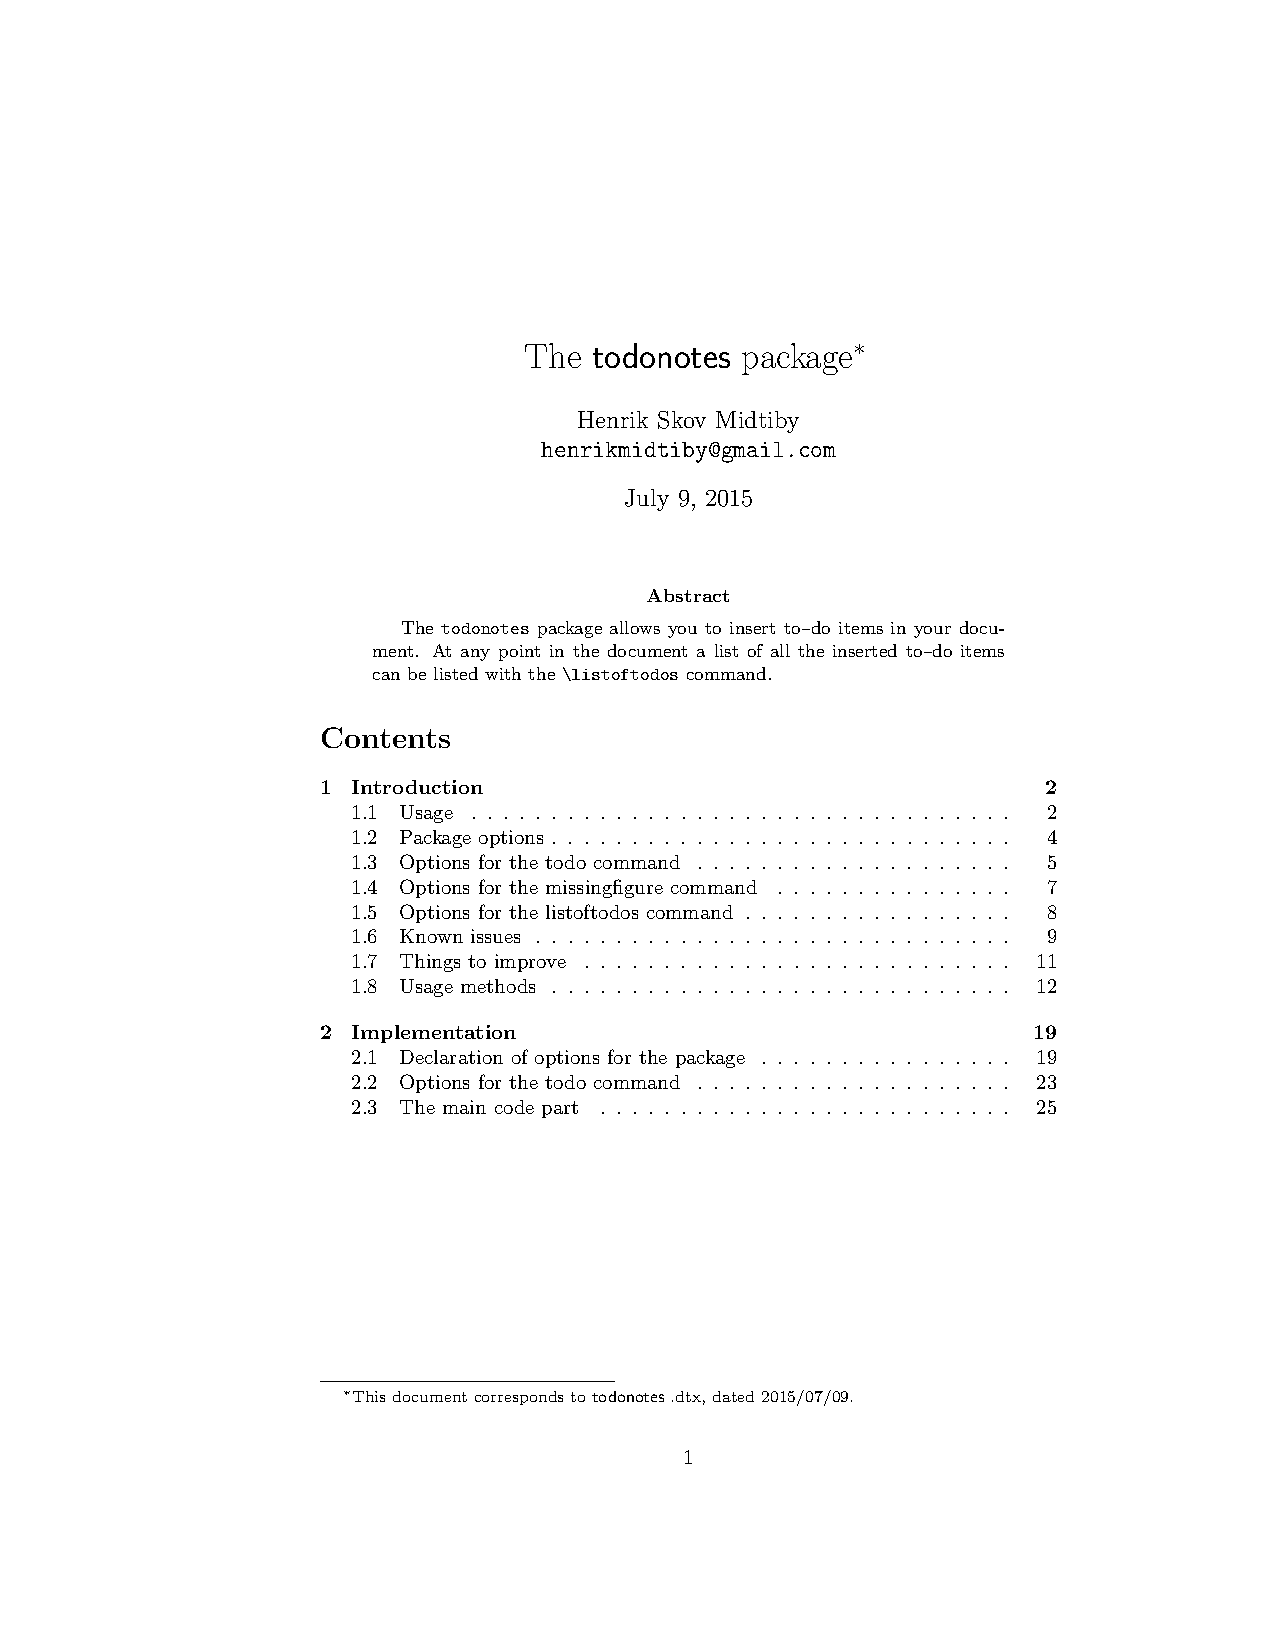
\includepdf[pages=1-3,scale=0.8,frame=true,pagecommand={}]{anexos/todonotes.pdf}

% ---
% Para incluir sem gerar a quebra de página inicial no anexo
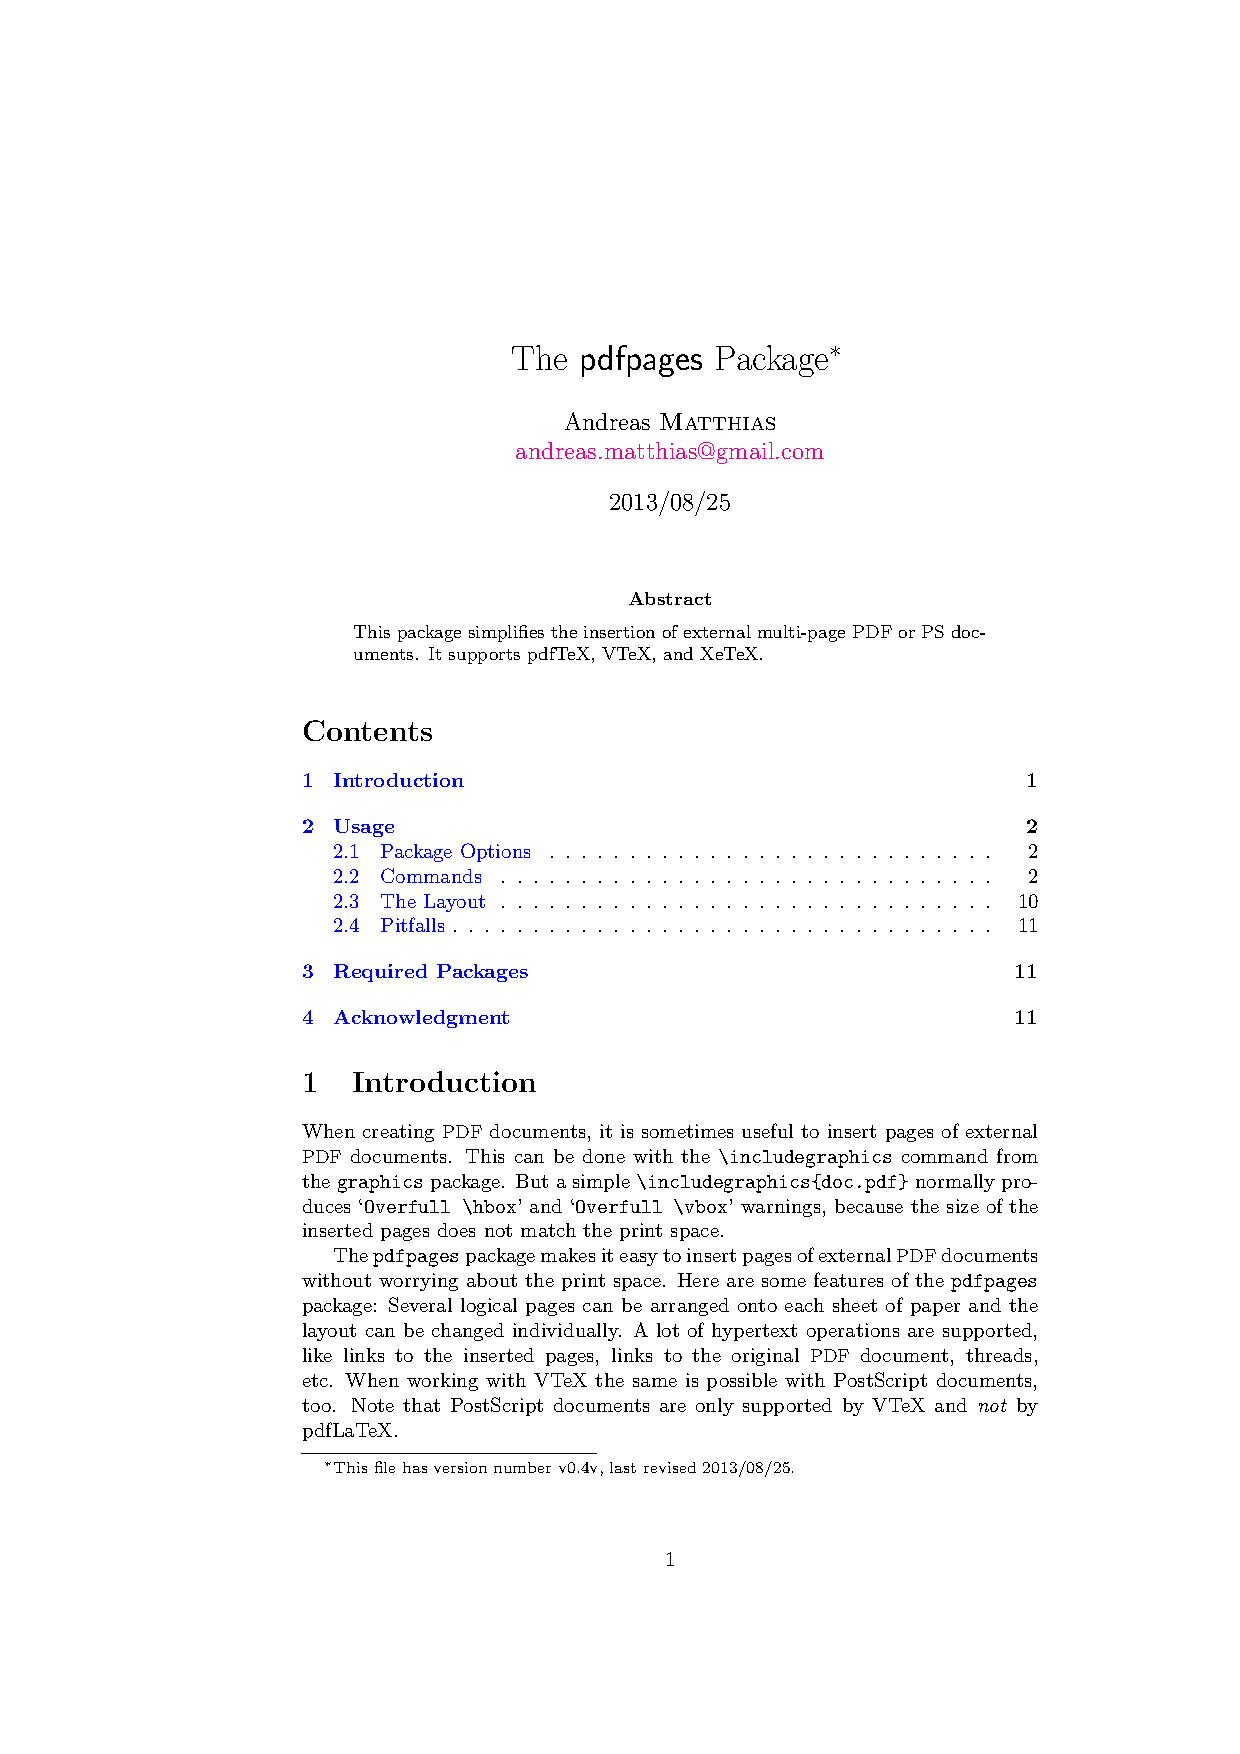
\includepdf[pages=1,scale=0.7,frame=true,pagecommand=\chapter{Manual pdfpages(parcial)}\label{manual-pdfpages}]{anexos/pdfpages.pdf}
\includepdf[pages=2-3,scale=0.8,frame=true,pagecommand={}]{anexos/pdfpages.pdf}

% ---
\chapter{Manual acronym(parcial)}
\index{pdf}
% somente algumas páginas para exemplo sem borda
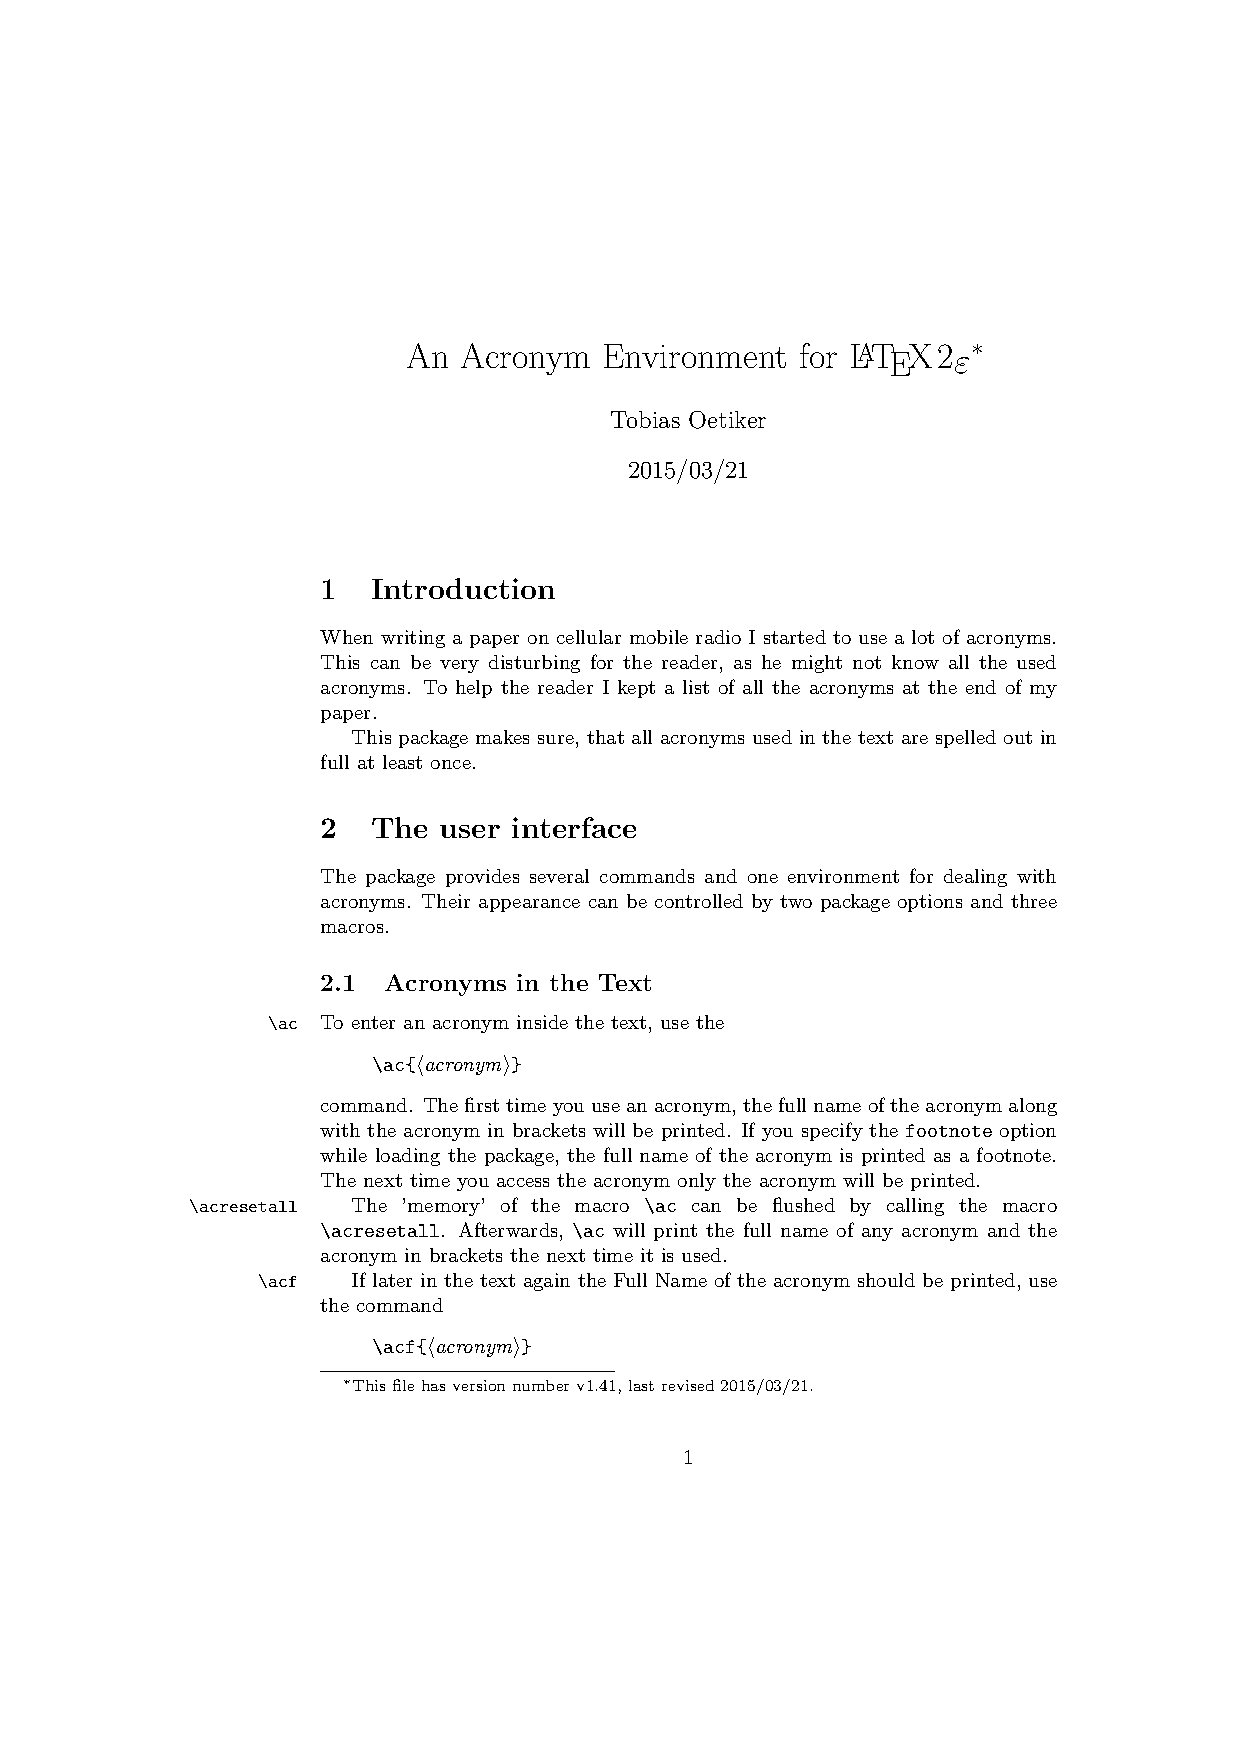
\includepdf[pages=1-3,frame=false,pagecommand={}]{anexos/acronym.pdf}



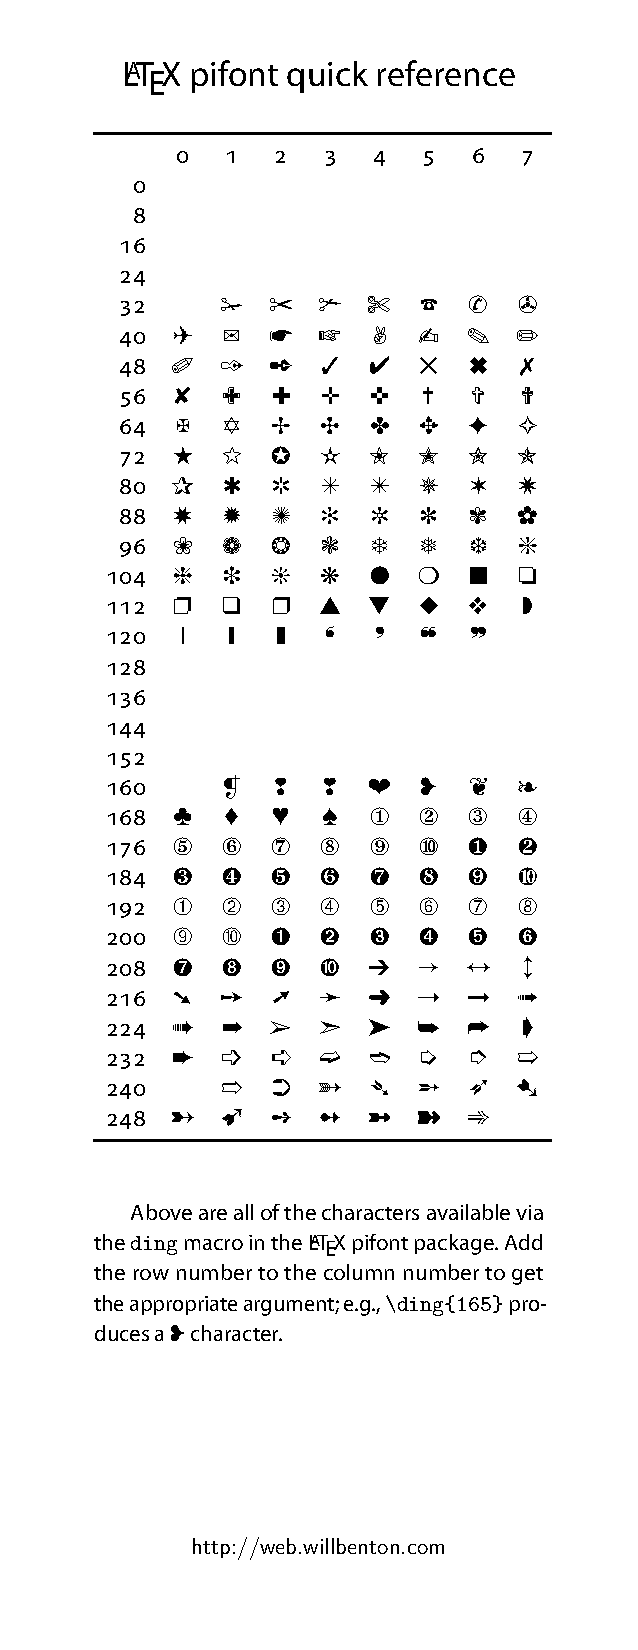
\includepdf[frame=true,scale=0.7,pagecommand=\chapter{Referência Rápida pifont}\label{pifont-quickref}]{anexos/pifont.pdf}


\end{anexosenv}

\DIFaddend 

\end{document}

